
%% bare_jrnl.tex
%% V1.3
%% 2007/01/11
%% by Michael Shell
%% see http://www.michaelshell.org/
%% for current contact information.
%%
%% This is a skeleton file demonstrating the use of IEEEtran.cls
%% (requires IEEEtran.cls version 1.7 or later) with an IEEE journal paper.
%%
%% Support sites:
%% http://www.michaelshell.org/tex/ieeetran/
%% http://www.ctan.org/tex-archive/macros/latex/contrib/IEEEtran/
%% and
%% http://www.ieee.org/



% *** Authors should verify (and, if needed, correct) their LaTeX system  ***
% *** with the testflow diagnostic prior to trusting their LaTeX platform ***
% *** with production work. IEEE's font choices can trigger bugs that do  ***
% *** not appear when using other class files.                            ***
% The testflow support page is at:
% http://www.michaelshell.org/tex/testflow/


%%*************************************************************************
%% Legal Notice:
%% This code is offered as-is without any warranty either expressed or
%% implied; without even the implied warranty of MERCHANTABILITY or
%% FITNESS FOR A PARTICULAR PURPOSE! 
%% User assumes all risk.
%% In no event shall IEEE or any contributor to this code be liable for
%% any damages or losses, including, but not limited to, incidental,
%% consequential, or any other damages, resulting from the use or misuse
%% of any information contained here.
%%
%% All comments are the opinions of their respective authors and are not
%% necessarily endorsed by the IEEE.
%%
%% This work is distributed under the LaTeX Project Public License (LPPL)
%% ( http://www.latex-project.org/ ) version 1.3, and may be freely used,
%% distributed and modified. A copy of the LPPL, version 1.3, is included
%% in the base LaTeX documentation of all distributions of LaTeX released
%% 2003/12/01 or later.
%% Retain all contribution notices and credits.
%% ** Modified files should be clearly indicated as such, including  **
%% ** renaming them and changing author support contact information. **
%%
%% File list of work: IEEEtran.cls, IEEEtran_HOWTO.pdf, bare_adv.tex,
%%                    bare_conf.tex, bare_jrnl.tex, bare_jrnl_compsoc.tex
%%*************************************************************************

% Note that the a4paper option is mainly intended so that authors in
% countries using A4 can easily print to A4 and see how their papers will
% look in print - the typesetting of the document will not typically be
% affected with changes in paper size (but the bottom and side margins will).
% Use the testflow package mentioned above to verify correct handling of
% both paper sizes by the user's LaTeX system.
%
% Also note that the "draftcls" or "draftclsnofoot", not "draft", option
% should be used if it is desired that the figures are to be displayed in
% draft mode.
%
\documentclass[journal]{IEEEtran}
\usepackage{blindtext}
\usepackage{graphicx}
\usepackage{zed-csp}
\usepackage[normalem]{ulem}
\usepackage[utf8]{inputenc}
\usepackage[english]{babel}
 
\usepackage{multicol}
\usepackage{multirow} 
 
 
\usepackage{amsthm}

\theoremstyle{definition}

\newtheorem{definition}{Definition}
\newtheorem{theorem}{Theorem}
\newtheorem{example}{Example}



 
\usepackage{listings}
\usepackage{color}
\usepackage{graphicx, subfigure}
\usepackage{caption}

\usepackage{algpseudocode}
 
\definecolor{codegreen}{rgb}{0,0.6,0}
\definecolor{codegray}{rgb}{0.5,0.5,0.5}
\definecolor{codepurple}{rgb}{0.58,0,0.82}
\definecolor{backcolour}{rgb}{0.95,0.95,0.92}
 
\lstdefinestyle{mystyle}{
    backgroundcolor=\color{backcolour},   
    commentstyle=\color{codegreen},
    keywordstyle=\color{magenta},
    numberstyle=\tiny\color{codegray},
    stringstyle=\color{codepurple},
    basicstyle=\footnotesize,
    breakatwhitespace=false,         
    breaklines=true,                 
    captionpos=b,                    
    keepspaces=true,                 
    numbers=left,                    
    numbersep=5pt,                  
    showspaces=false,                
    showstringspaces=false,
    showtabs=false,                  
    tabsize=2
}
 
\lstset{style=mystyle}
% Some very useful LaTeX packages include:
% (uncomment the ones you want to load)


% *** MISC UTILITY PACKAGES ***
%
%\usepackage{ifpdf}
% Heiko Oberdiek's ifpdf.sty is very useful if you need conditional
% compilation based on whether the output is pdf or dvi.
% usage:
% \ifpdf
%   % pdf code
% \else
%   % dvi code
% \fi
% The latest version of ifpdf.sty can be obtained from:
% http://www.ctan.org/tex-archive/macros/latex/contrib/oberdiek/
% Also, note that IEEEtran.cls V1.7 and later provides a builtin
% \ifCLASSINFOpdf conditional that works the same way.
% When switching from latex to pdflatex and vice-versa, the compiler may
% have to be run twice to clear warning/error messages.






% *** CITATION PACKAGES ***
%
%\usepackage{cite}
% cite.sty was written by Donald Arseneau
% V1.6 and later of IEEEtran pre-defines the format of the cite.sty package
% \cite{} output to follow that of IEEE. Loading the cite package will
% result in citation numbers being automatically sorted and properly
% "compressed/ranged". e.g., [1], [9], [2], [7], [5], [6] without using
% cite.sty will become [1], [2], [5]--[7], [9] using cite.sty. cite.sty's
% \cite will automatically add leading space, if needed. Use cite.sty's
% noadjust option (cite.sty V3.8 and later) if you want to turn this off.
% cite.sty is already installed on most LaTeX systems. Be sure and use
% version 4.0 (2003-05-27) and later if using hyperref.sty. cite.sty does
% not currently provide for hyperlinked citations.
% The latest version can be obtained at:
% http://www.ctan.org/tex-archive/macros/latex/contrib/cite/
% The documentation is contained in the cite.sty file itself.






% *** GRAPHICS RELATED PACKAGES ***
%
\ifCLASSINFOpdf
  % \usepackage[pdftex]{graphicx}
  % declare the path(s) where your graphic files are
  % \graphicspath{{../pdf/}{../jpeg/}}
  % and their extensions so you won't have to specify these with
  % every instance of \includegraphics
  % \DeclareGraphicsExtensions{.pdf,.jpeg,.png}
\else
  % or other class option (dvipsone, dvipdf, if not using dvips). graphicx
  % will default to the driver specified in the system graphics.cfg if no
  % driver is specified.
  % \usepackage[dvips]{graphicx}
  % declare the path(s) where your graphic files are
  % \graphicspath{{../eps/}}
  % and their extensions so you won't have to specify these with
  % every instance of \includegraphics
  % \DeclareGraphicsExtensions{.eps}
\fi
% graphicx was written by David Carlisle and Sebastian Rahtz. It is
% required if you want graphics, photos, etc. graphicx.sty is already
% installed on most LaTeX systems. The latest version and documentation can
% be obtained at: 
% http://www.ctan.org/tex-archive/macros/latex/required/graphics/
% Another good source of documentation is "Using Imported Graphics in
% LaTeX2e" by Keith Reckdahl which can be found as epslatex.ps or
% epslatex.pdf at: http://www.ctan.org/tex-archive/info/
%
% latex, and pdflatex in dvi mode, support graphics in encapsulated
% postscript (.eps) format. pdflatex in pdf mode supports graphics
% in .pdf, .jpeg, .png and .mps (metapost) formats. Users should ensure
% that all non-photo figures use a vector format (.eps, .pdf, .mps) and
% not a bitmapped formats (.jpeg, .png). IEEE frowns on bitmapped formats
% which can result in "jaggedy"/blurry rendering of lines and letters as
% well as large increases in file sizes.
%
% You can find documentation about the pdfTeX application at:
% http://www.tug.org/applications/pdftex





% *** MATH PACKAGES ***
%
%\usepackage[cmex10]{amsmath}
% A popular package from the American Mathematical Society that provides
% many useful and powerful commands for dealing with mathematics. If using
% it, be sure to load this package with the cmex10 option to ensure that
% only type 1 fonts will utilized at all point sizes. Without this option,
% it is possible that some math symbols, particularly those within
% footnotes, will be rendered in bitmap form which will result in a
% document that can not be IEEE Xplore compliant!
%
% Also, note that the amsmath package sets \interdisplaylinepenalty to 10000
% thus preventing page breaks from occurring within multiline equations. Use:
%\interdisplaylinepenalty=2500
% after loading amsmath to restore such page breaks as IEEEtran.cls normally
% does. amsmath.sty is already installed on most LaTeX systems. The latest
% version and documentation can be obtained at:
% http://www.ctan.org/tex-archive/macros/latex/required/amslatex/math/





% *** SPECIALIZED LIST PACKAGES ***
%
%\usepackage{algorithmic}
% algorithmic.sty was written by Peter Williams and Rogerio Brito.
% This package provides an algorithmic environment fo describing algorithms.
% You can use the algorithmic environment in-text or within a figure
% environment to provide for a floating algorithm. Do NOT use the algorithm
% floating environment provided by algorithm.sty (by the same authors) or
% algorithm2e.sty (by Christophe Fiorio) as IEEE does not use dedicated
% algorithm float types and packages that provide these will not provide
% correct IEEE style captions. The latest version and documentation of
% algorithmic.sty can be obtained at:
% http://www.ctan.org/tex-archive/macros/latex/contrib/algorithms/
% There is also a support site at:
% http://algorithms.berlios.de/index.html
% Also of interest may be the (relatively newer and more customizable)
% algorithmicx.sty package by Szasz Janos:
% http://www.ctan.org/tex-archive/macros/latex/contrib/algorithmicx/




% *** ALIGNMENT PACKAGES ***
%
%\usepackage{array}
% Frank Mittelbach's and David Carlisle's array.sty patches and improves
% the standard LaTeX2e array and tabular environments to provide better
% appearance and additional user controls. As the default LaTeX2e table
% generation code is lacking to the point of almost being broken with
% respect to the quality of the end results, all users are strongly
% advised to use an enhanced (at the very least that provided by array.sty)
% set of table tools. array.sty is already installed on most systems. The
% latest version and documentation can be obtained at:
% http://www.ctan.org/tex-archive/macros/latex/required/tools/


%\usepackage{mdwmath}
%\usepackage{mdwtab}
% Also highly recommended is Mark Wooding's extremely powerful MDW tools,
% especially mdwmath.sty and mdwtab.sty which are used to format equations
% and tables, respectively. The MDWtools set is already installed on most
% LaTeX systems. The lastest version and documentation is available at:
% http://www.ctan.org/tex-archive/macros/latex/contrib/mdwtools/


% IEEEtran contains the IEEEeqnarray family of commands that can be used to
% generate multiline equations as well as matrices, tables, etc., of high
% quality.


%\usepackage{eqparbox}
% Also of notable interest is Scott Pakin's eqparbox package for creating
% (automatically sized) equal width boxes - aka "natural width parboxes".
% Available at:
% http://www.ctan.org/tex-archive/macros/latex/contrib/eqparbox/





% *** SUBFIGURE PACKAGES ***
%\usepackage[tight,footnotesize]{subfigure}
% subfigure.sty was written by Steven Douglas Cochran. This package makes it
% easy to put subfigures in your figures. e.g., "Figure 1a and 1b". For IEEE
% work, it is a good idea to load it with the tight package option to reduce
% the amount of white space around the subfigures. subfigure.sty is already
% installed on most LaTeX systems. The latest version and documentation can
% be obtained at:
% http://www.ctan.org/tex-archive/obsolete/macros/latex/contrib/subfigure/
% subfigure.sty has been superceeded by subfig.sty.



%\usepackage[caption=false]{caption}
%\usepackage[font=footnotesize]{subfig}
% subfig.sty, also written by Steven Douglas Cochran, is the modern
% replacement for subfigure.sty. However, subfig.sty requires and
% automatically loads Axel Sommerfeldt's caption.sty which will override
% IEEEtran.cls handling of captions and this will result in nonIEEE style
% figure/table captions. To prevent this problem, be sure and preload
% caption.sty with its "caption=false" package option. This is will preserve
% IEEEtran.cls handing of captions. Version 1.3 (2005/06/28) and later 
% (recommended due to many improvements over 1.2) of subfig.sty supports
% the caption=false option directly:
%\usepackage[caption=false,font=footnotesize]{subfig}
%
% The latest version and documentation can be obtained at:
% http://www.ctan.org/tex-archive/macros/latex/contrib/subfig/
% The latest version and documentation of caption.sty can be obtained at:
% http://www.ctan.org/tex-archive/macros/latex/contrib/caption/




% *** FLOAT PACKAGES ***
%
%\usepackage{fixltx2e}
% fixltx2e, the successor to the earlier fix2col.sty, was written by
% Frank Mittelbach and David Carlisle. This package corrects a few problems
% in the LaTeX2e kernel, the most notable of which is that in current
% LaTeX2e releases, the ordering of single and double column floats is not
% guaranteed to be preserved. Thus, an unpatched LaTeX2e can allow a
% single column figure to be placed prior to an earlier double column
% figure. The latest version and documentation can be found at:
% http://www.ctan.org/tex-archive/macros/latex/base/



%\usepackage{stfloats}
% stfloats.sty was written by Sigitas Tolusis. This package gives LaTeX2e
% the ability to do double column floats at the bottom of the page as well
% as the top. (e.g., "\begin{figure*}[!b]" is not normally possible in
% LaTeX2e). It also provides a command:
%\fnbelowfloat
% to enable the placement of footnotes below bottom floats (the standard
% LaTeX2e kernel puts them above bottom floats). This is an invasive package
% which rewrites many portions of the LaTeX2e float routines. It may not work
% with other packages that modify the LaTeX2e float routines. The latest
% version and documentation can be obtained at:
% http://www.ctan.org/tex-archive/macros/latex/contrib/sttools/
% Documentation is contained in the stfloats.sty comments as well as in the
% presfull.pdf file. Do not use the stfloats baselinefloat ability as IEEE
% does not allow \baselineskip to stretch. Authors submitting work to the
% IEEE should note that IEEE rarely uses double column equations and
% that authors should try to avoid such use. Do not be tempted to use the
% cuted.sty or midfloat.sty packages (also by Sigitas Tolusis) as IEEE does
% not format its papers in such ways.


%\ifCLASSOPTIONcaptionsoff
%  \usepackage[nomarkers]{endfloat}
% \let\MYoriglatexcaption\caption
% \renewcommand{\caption}[2][\relax]{\MYoriglatexcaption[#2]{#2}}
%\fi
% endfloat.sty was written by James Darrell McCauley and Jeff Goldberg.
% This package may be useful when used in conjunction with IEEEtran.cls'
% captionsoff option. Some IEEE journals/societies require that submissions
% have lists of figures/tables at the end of the paper and that
% figures/tables without any captions are placed on a page by themselves at
% the end of the document. If needed, the draftcls IEEEtran class option or
% \CLASSINPUTbaselinestretch interface can be used to increase the line
% spacing as well. Be sure and use the nomarkers option of endfloat to
% prevent endfloat from "marking" where the figures would have been placed
% in the text. The two hack lines of code above are a slight modification of
% that suggested by in the endfloat docs (section 8.3.1) to ensure that
% the full captions always appear in the list of figures/tables - even if
% the user used the short optional argument of \caption[]{}.
% IEEE papers do not typically make use of \caption[]'s optional argument,
% so this should not be an issue. A similar trick can be used to disable
% captions of packages such as subfig.sty that lack options to turn off
% the subcaptions:
% For subfig.sty:
% \let\MYorigsubfloat\subfloat
% \renewcommand{\subfloat}[2][\relax]{\MYorigsubfloat[]{#2}}
% For subfigure.sty:
% \let\MYorigsubfigure\subfigure
% \renewcommand{\subfigure}[2][\relax]{\MYorigsubfigure[]{#2}}
% However, the above trick will not work if both optional arguments of
% the \subfloat/subfig command are used. Furthermore, there needs to be a
% description of each subfigure *somewhere* and endfloat does not add
% subfigure captions to its list of figures. Thus, the best approach is to
% avoid the use of subfigure captions (many IEEE journals avoid them anyway)
% and instead reference/explain all the subfigures within the main caption.
% The latest version of endfloat.sty and its documentation can obtained at:
% http://www.ctan.org/tex-archive/macros/latex/contrib/endfloat/
%
% The IEEEtran \ifCLASSOPTIONcaptionsoff conditional can also be used
% later in the document, say, to conditionally put the References on a 
% page by themselves.





% *** PDF, URL AND HYPERLINK PACKAGES ***
%
\usepackage{url}
% url.sty was written by Donald Arseneau. It provides better support for
% handling and breaking URLs. url.sty is already installed on most LaTeX
% systems. The latest version can be obtained at:
% http://www.ctan.org/tex-archive/macros/latex/contrib/misc/
% Read the url.sty source comments for usage information. Basically,
% \url{my_url_here}.



% Macros for proof-reading
\usepackage[normalem]{ulem} % for \sout
\usepackage{xcolor}
\newcommand{\ra}{$\rightarrow$}
\newcommand{\ugh}[1]{\textcolor{red}{\uwave{#1}}} % please rephrase
\newcommand{\ins}[1]{\textcolor{blue}{\uline{#1}}} % please insert
\newcommand{\del}[1]{\textcolor{red}{\sout{#1}}} % please delete
\newcommand{\chg}[2]{\textcolor{red}{\sout{#1}}{\ra}\textcolor{blue}{\uline{#2}}} % please change

% Put edit comments in a really ugly standout display
\usepackage{ifthen}
%\usepackage{amssymb}
\usepackage{amsfonts}
\newboolean{showcomments}
\setboolean{showcomments}{true} % toggle to show or hide comments
\ifthenelse{\boolean{showcomments}}
  {\newcommand{\nb}[2]{
    \fcolorbox{gray}{yellow}{\bfseries\sffamily\scriptsize#1}
    {\sf\small$\blacktriangleright$\textit{#2}$\blacktriangleleft$}
   }
   \newcommand{\version}{\emph{\scriptsize$-$working$-$}}
  }
  {\newcommand{\nb}[2]{}
   \newcommand{\version}{}
  }

\newcommand\darko[1]{\nb{Darko}{#1}}
\newcommand\patrizio[1]{\nb{Patrizio}{#1}}
\newcommand\ivano[1]{\nb{Ivano}{#1}}
\newcommand\todo[1]{\nb{Todo}{#1}}
\newcommand\lookinto[1]{\nb{Look Into}{#1}}




% *** Do not adjust lengths that control margins, column widths, etc. ***
% *** Do not use packages that alter fonts (such as pslatex).         ***
% There should be no need to do such things with IEEEtran.cls V1.6 and later.
% (Unless specifically asked to do so by the journal or conference you plan
% to submit to, of course. )


% correct bad hyphenation here
\hyphenation{op-tical net-works semi-conduc-tor}


\begin{document}
%
% paper title
% can use linebreaks \\ within to get better formatting as desired
\title{IEEE Journal Template Example}
%
%
% author names and IEEE memberships
% note positions of commas and nonbreaking spaces ( ~ ) LaTeX will not break
% a structure at a ~ so this keeps an author's name from being broken across
% two lines.
% use \thanks{} to gain access to the first footnote area
% a separate \thanks must be used for each paragraph as LaTeX2e's \thanks
% was not built to handle multiple paragraphs
%

\author{Michael~Shell,~\IEEEmembership{Member,~IEEE,}
        John~Doe,~\IEEEmembership{Fellow,~OSA,}
        and~Jane~Doe,~\IEEEmembership{Life~Fellow,~IEEE}% <-this % stops a space
\thanks{M. Shell is with the Department
of Electrical and Computer Engineering, Georgia Institute of Technology, Atlanta,
GA, 30332 USA e-mail: (see http://www.michaelshell.org/contact.html).}% <-this % stops a space
\thanks{J. Doe and J. Doe are with Anonymous University.}% <-this % stops a space
\thanks{Manuscript received April 19, 2005; revised January 11, 2007.}}

% note the % following the last \IEEEmembership and also \thanks - 
% these prevent an unwanted space from occurring between the last author name
% and the end of the author line. i.e., if you had this:
% 
% \author{....lastname \thanks{...} \thanks{...} }
%                     ^------------^------------^----Do not want these spaces!
%
% a space would be appended to the last name and could cause every name on that
% line to be shifted left slightly. This is one of those "LaTeX things". For
% instance, "\textbf{A} \textbf{B}" will typeset as "A B" not "AB". To get
% "AB" then you have to do: "\textbf{A}\textbf{B}"
% \thanks is no different in this regard, so shield the last } of each \thanks
% that ends a line with a % and do not let a space in before the next \thanks.
% Spaces after \IEEEmembership other than the last one are OK (and needed) as
% you are supposed to have spaces between the names. For what it is worth,
% this is a minor point as most people would not even notice if the said evil
% space somehow managed to creep in.



% The paper headers
\markboth{Journal of \LaTeX\ Class Files,~Vol.~6, No.~1, January~2007}%
{Shell \MakeLowercase{\textit{et al.}}: Bare Demo of IEEEtran.cls for Journals}
% The only time the second header will appear is for the odd numbered pages
% after the title page when using the twoside option.
% 
% *** Note that you probably will NOT want to include the author's ***
% *** name in the headers of peer review papers.                   ***
% You can use \ifCLASSOPTIONpeerreview for conditional compilation here if
% you desire.




% If you want to put a publisher's ID mark on the page you can do it like
% this:
%\IEEEpubid{0000--0000/00\$00.00~\copyright~2007 IEEE}
% Remember, if you use this you must call \IEEEpubidadjcol in the second
% column for its text to clear the IEEEpubid mark.



% use for special paper notices
%\IEEEspecialpapernotice{(Invited Paper)}




% make the title area
\maketitle


\begin{abstract}
%\boldmath




\end{abstract}
% IEEEtran.cls defaults to using nonbold math in the Abstract.
% This preserves the distinction between vectors and scalars. However,
% if the journal you are submitting to favors bold math in the abstract,
% then you can use LaTeX's standard command \boldmath at the very start
% of the abstract to achieve this. Many IEEE journals frown on math
% in the abstract anyway.

% Note that keywords are not normally used for peerreview papers.
\begin{IEEEkeywords}
IEEEtran, journal, \LaTeX, paper, template.
\end{IEEEkeywords}






% For peer review papers, you can put extra information on the cover
% page as needed:
% \ifCLASSOPTIONpeerreview
% \begin{center} \bfseries EDICS Category: 3-BBND \end{center}
% \fi
%
% For peerreview papers, this IEEEtran command inserts a page break and
% creates the second title. It will be ignored for other modes.
\IEEEpeerreviewmaketitle

\section{Introduction}
\ivano{this section will need a strong rewriting step (e.g., adding proper references, explaining better the concepts, contributions, etc.), but we can do it later.}
 Mobile Multi-Robot Systems (MMRSs) are an emerging class of systems that adapt their behavior at run-time to achieve specific goals. They are represented by a set of mobile robots operating as a team with other agents (with agents we refer to generic robots, ground stations, or even humans) in a shared environment. 
 
 %In the literature, a variety of definitions exists defining the term robot [4–6]\patrizio{put proper references}. All of them share the following concept: a robot is an intelligent device with a certain degree of autonomy that contains sensors, control systems, manipulators, power supplies and software all working together to perform the required tasks. Under this perspective, a mobile robot represents a robotic system consisting of a SW/HW platform carried around by locomotive elements and able to perform tasks in different contexts. The kind of locomotion that the robot is able to perform is primarily decided upon the environment (aquatic, aerial or terrestrial) in which the robot will be operating [7].\patrizio{put proper reference}  Mobility gives robots enhanced operative capabilities, but at the same time increases complexity and brings additional challenges.
 

 MMRSs should be able to operate under dynamic, uncontrollable and partially or fully unknown environments.
%\ivano{add a couple of examples}). 
That introduces a set of uncertainties resulting from the incomplete knowledge of the run-time structure of MMRS (ex. number of agents performing a particular task in a specific moment) and the environment in which the MMRS operates. Incomplete knowledge of the run-time structure of MMRS comes from its openness. By \chg{"}{``}openness" we mean that new entities can join or leave the system at run-time. Incomplete knowledge of the environment comes from its dynamics and uncontrollability (e.g., a bird flying in the environment). The consideration of the environment when specifying the system comes due to the fact that a mission is always associated with a physical context where it is happening, so how a system will perform a mission strongly depends on the environment where it operates (e.g., the system will operate differently in environments with smooth vs. rough surface, environments  with a lot of static obstacles vs environments with a small number of obstacles etc). 
%We consider the environment at design-time we define mission because (usually) a house does not move at runtime, so the planning of the trajectories can benefit from knowing this info beforehand) as to define a mission we always locate it in a specific  in our de part of the )\ivano{explain why the knowledge is incomplete at run-time, and why it will always be like that, that is: there is some information that is not known at design time by definition (e.g., a bird flying into a drone)} and the environment at design time \ivano{what do you mean by environment here? The physical environment? If it is like that, then you have to explain why you consider the environment also at design time since many approaches do not make any assumptions on it at design time. We do it because (usually) a house does not move at runtime, so the planning of the trajectories can benefit from knowing this info beforehand)}.

Handling uncertainty upfront is often infeasible (or expensive). This means we need to deal with it when the knowledge becomes available at runtime. 
Hence, the construction of MMRSs is significantly more challenging than traditional systems due to  their mission-criticality (meaning a loss of resources can lead to possible reduction in mission effectiveness) and their safety-criticality (meaning a failure or defective design could cause a risk to human life and the environment). Commercialisation and adoption of MMRSs in dynamic environments will only occur if safety aspects are considered and incorporated as first class concerns in the design of the system. Certification bodies should assure some type of safety certification that relies on a complete understanding of the system. However, for mobile robots that operate in dynamic environments \chg{its}{it is} quite challenging to consider all variants of the overall system due to their adaptive behaviour. Hence, having the ability to analyse and reason about safety independently from the mission 
%However, that way we do not have any utilization of the system, so finding the right trade-off between how much safe a system should be and how much and which part of the mission is completed 
requires a clear separation of concerns between safety and mission related issues. 

System designers should be able to precisely specify different adaptation solutions with specific guarantees for the different agents in MMRSs in order to ensure high operational confidence. Moreover, they should be able to craft different adaptation solutions that can be reused across missions, projects, and organizations to minimize the developing cost.
%For that, system designers should be able to flexible and precise "enough" describe, compare, and evaluate alternative adaptation choices for the different constituents of MMRSs.
However, researchers and practitioners have been struggling with the lack of models, methods, techniques and tools that are flexible and precise "enough" to describe, compare, and evaluate alternative adaptation solutions.
%flexible and precise "enough"  to be used for describing, comparing, and evaluating alternative adaptation choices for agents in MMRSs.
\patrizio{Here there should be a brief summary of the sttae of the art and a clear explanation of what is missing.}
With our work, 
%\sout{having agents that have local knowledge about the changing system and environment and operate in some context} we want to address \sout{variety of} 
we address the aforementioned challenges and design a modeling framework that supports \textbf{execution of missions} in MMRSs and:
\begin{enumerate}
\item provides intuitive and precise specification and description of the run-time behaviour of different agents in the system. 
\item makes a clear separation between mission-related and safety-related adaptation mechanisms 
\item ensures guarantees about the behaviour of the system. 
\end{enumerate}

\patrizio{Here there should be a summary of the paper}


%To perform adaptation, the system needs to decide how to adapt. There might be different ways for an adaptation to be performed. That \ivano{that whay?} requires identification of variability points of the system at design-time \ivano{this is already part of the solution.}. Variability among MMRSs is multi-dimensional since changes can occur both vertically (within domain and specification of a single agent) as well as horizontally (among different MMRSs’ agents). While many existing approaches are tackling the challenges emerging out of the vertical variability (\todo{find reference}) and provide solutions to problems associated with a single robot, we want to complement those approaches and tackle problems where a single robot can not perform the mission alone because of lack of resources. (e.g., pictures around big open space should be taken, but one drone cannot finish the mission because of lack of battery power).
%In this work, we focus primarily on horizontal variability and the challenges that emerge out of it \ivano{here the fact that we complement other approaches is missing}.  
%\ivano{This sentence sounds really as a big limitation of our approach, we have to rephrase it so that we tell that many approaches exist for vertical variability, but we want to complement them in order to solve a much interesting problem: the one related to collective adaptation}. 
%In order to better understand the nature of this problem and the challenges that arise  in MMRSs, we identify two dimensions of horizontal variability  as discussed in \todo{[reference needed]}: system variability, and mission variability. 

%\ivano{not clear, add examples of SW/HW variability and mission planning/execution variability}
 %\ivano{why the following two dimensions? Where do they come from?}:
%\textbf{System variability} Currently robotic software researchers and engineers mainly focus on delivering highly efficient implementations of control applications for specific platforms in well-defined operational environments [4]. However, the desire to tackle performance issues has resulted in neglecting other relevant quality attributes of a system, such as reusability, interoperability, and maintainability [4]. 
%As a consequence, available solutions, both software and hardware, are incredibly heterogeneous. Additionally, neither software nor hardware has been truly standardized yet, thus making the development of MMRSs involving heterogeneous robots very intricate and somewhat frustrating for developers that find themselves compelled in re-inventing the wheel over and over again. In point of fact, reuse of software components and their integration within a specific robotic application is not properly supported either.

%\textbf{Mission variability.} MMRSs are required to operate in diverse civilian missions, such as damage assessment after earthquakes, atmospheric research etc. Each of these scenarios introduces new forms of uncertainty which comes from two sources: (i) the resources that these systems use (energy, memory, connection capabilities, etc.) and their change over time and (ii) new contextual elements that can appear or disappear in the physical context at run-time (ex. animals walking in the environment, etc.). The variety of missions discussed above implies an extensive assortment of interaction scenarios, each with particular quality requirements. 
%\patrizio{The part above is too long for an introdcution. Please consider to move part of the text about MMRSs to a background or context section.} \\

%As discussed in \todo{[citation needed]}, we can identify challenges that emerge out of both dimensions of horizontal variability and conclude that 

%\ivano{what is the link between (system and mission) variability and the two global objectives?}




%To solve these problem we  The motivation behind the work is to describe collective adaptation behavior of MMRSs in a formal and precise way.  


\section{Motivating Scenario}
\label{sec:motivation}
% - drones to cover an area, they are autonomous with their goals [IM]

%\patrizio{We might probably change the motivating example. In fact, the assumption of FlyAQ that drones have assigned and exclusive areas is too strong for this paper. With no interactions of drones, in fact, there no need of replanning. Basically, I propose to change the bottom of the figure} 
In this section, we describe  a motivating scenario of a carbon dioxide monitoring system (Figure~\ref{fig:Scenario}). This scenario will be used as a running example to explain details of the approach.
Figure~\ref{fig:Scenario} shows a mission in which three robots, specifically three Unmanned Autonomous Vehicles (UAVs), have to monitor the CO2 levels within a geographical area; the team of UAVs has to sense the CO2 level of each geographical point in a grid composed of cells of size $10x10$ meters. The mission is considered as successfully completed if the whole area has been fully monitored. %The figure also shows the places that have been identified as home positions of each UAV. The home position of a UAV is the geographical position where the UAV has to come back at the end of the mission.
%The mission specification contains also other contextual information, such as obstacles, no fly zones, and emergency places where UAVs can safely land in case of problems. 
Starting from this very high-level description of the mission, the configurations and flight plans for the  UAVs can be automatically generated. Once configured, these UAVs perform the mission by flying from their initial position to the border of the monitoring area. Then, each UAV starts monitoring a specific sub-area so that the whole team can cover the entire area in parallel. A sub-area can be decomposed in number of blocks.
 A block is the smallest measurable unit for the mission region. Each block is assigned a unique identifier. We represent the size of an area using the number of blocks along each dimension. 

The bottom side of Figure~\ref{fig:Scenario} shows the mission execution of three UAVs. Each UAV is executing its corresponding behaviour to cover  its part of the mission. The black region is the region that has been monitored by the corresponding UAVs.
%performed their mission i.e. they visited that particular area.}
The region with dots represents the region that should be monitored by the UAV with dots, the region with horizontal stripes is the region that should be monitored by the UAV  with horizontal stripes and the  region with vertical stripes is the region that should be monitored by the UAV with vertical stripes. 

%\patrizio{please rewrite} The other regions that have different colour are the regions for which the UAVs should perform the mission in the future, where the colour of the UAV is the same with the colour of the region it should visit.\patrizio{this sentence can be simplified. Moreover, it's not a good idea to use colors to distinguish the areas. This will be not readable when printed black and white.}
%information which region should visit.
%while the other colours information which UAV should visit region. 

Let us assume that a UAV $u_x$ (the UAV with dots on Figure~\ref{fig:Scenario}) of the team $U$ must reach a target geographical position $p$ and it identifies an obstacle along its trajectory towards $p$; if the obstacle is avoidable (e.g., a tree), then $u_x$ adapts its trajectory so that it avoids the obstacle to reach $p$; if the obstacle cannot be easily avoided (e.g., the large white object on Figure~\ref{fig:Scenario},
%\patrizio{I don't see this object in the figure})
then the behaviours of $u_x$ and some other UAVs in $U$ are adapted so that the position $p$ is still covered by another UAV $u_i \in U$ and $u_x$ can cover some other points within the area.  

\begin{figure}[h]

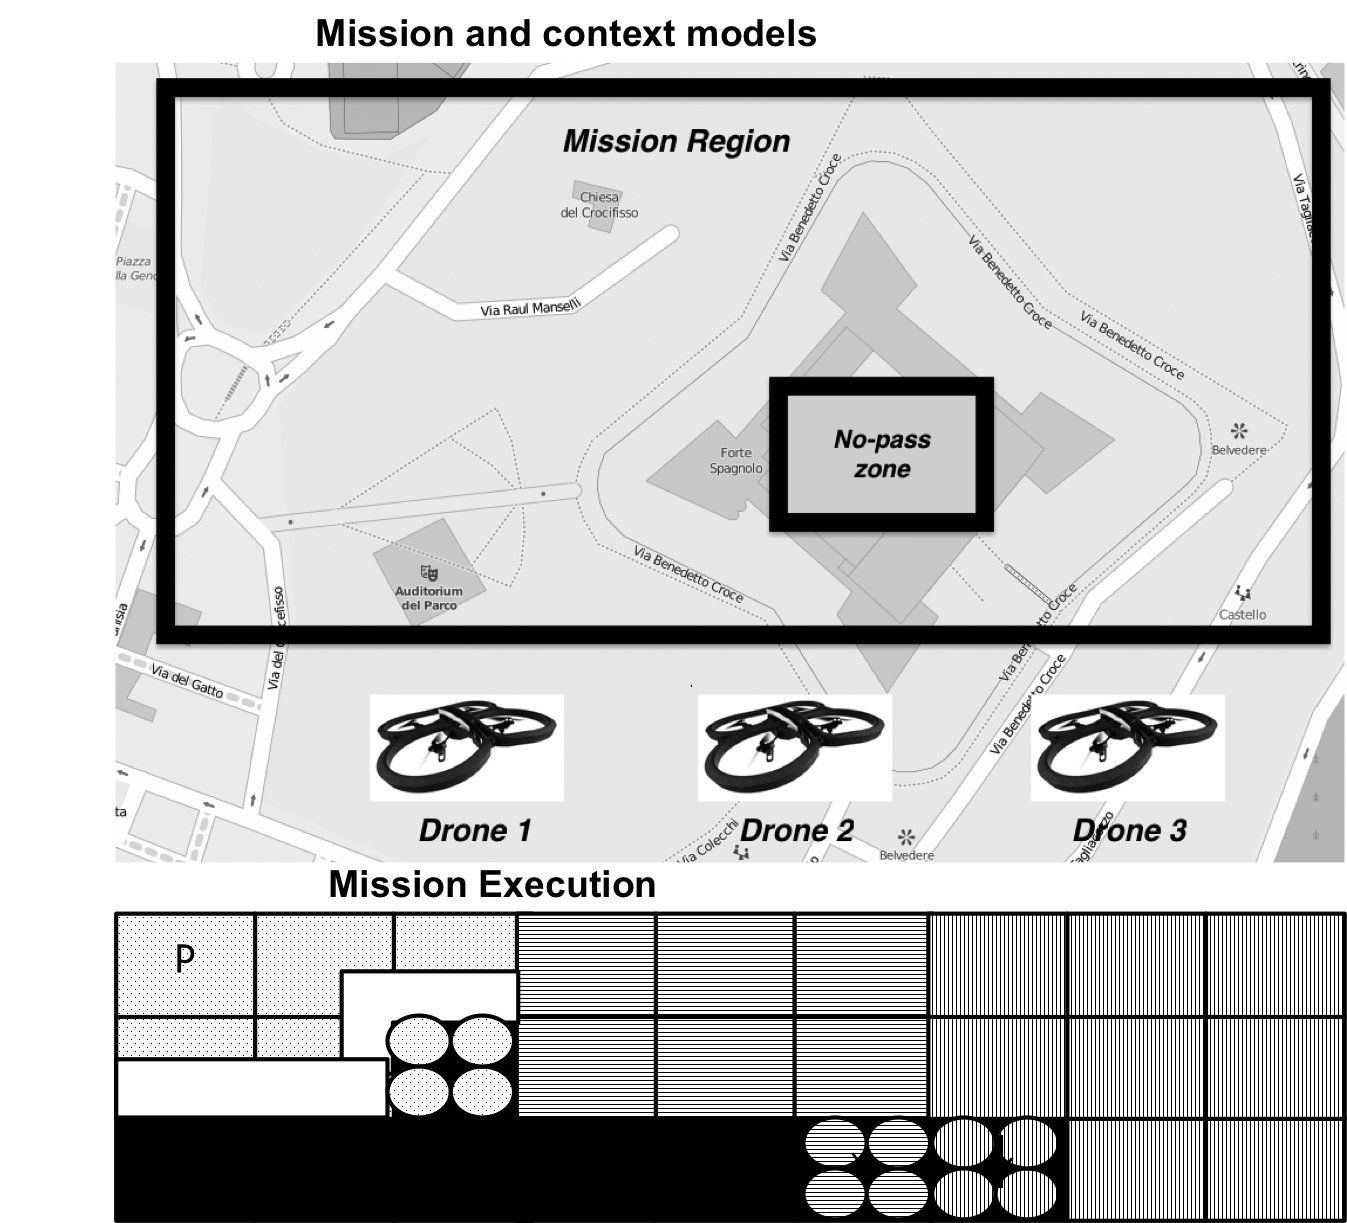
\includegraphics[width=3.25in]{Figures/Scenario_M.png}
\label{fig:second}
\caption{Motivating Scenario}\label{fig:Scenario}
\end{figure}


  


\section{Background}




%\subsection{Preliminaries}

In order to explain our framework we
start introducing some basic concepts
%\ugh{the notion of some basic concepts} 
that are used through out the paper.
%In this section, we formalize the definitions needed for the rest of
%the paper and represent concepts that will be used later on.\patrizio{two sentences that say almost the same}

\subsection{Design-time Elements: Terminology \& Definitions}


Let $Coordinates = \{(x,y,z) | x,y,z \in R\}$  be the universal set of geographical coordinates where the mission takes place; for $c \in Coordinates$, $c.x$ denotes the longitude of c, $c.y$ is the latitude,
and $c.z$ is the altitude. 
To represent the mission and the context in which a MMRS performs the mission we define a region as a generic term for defining geometric shapes in the environment. 

\begin{definition}[Region]
%\ivano{don't we need an additional element in region for describing its type (obstacle vs no-pass vs mission region)? Here we should also characterize the relationship between the x, y, z, I suspect that here you would like to say that they identify a polygon in the 2D environment or a polyhedron in the 3D one.}
A region $R=(P, t)$ is a pair where $P \in Coordinates$ 
%subset of Coordinates
%in the three dimensional xyz-plane
denotes a geometric shape in the environment (ex. it can identify a polygon in the 2D environment or a polyhedron in the 3D one) and $t$  defines the type of the region (ex. obstacle,  no-pass zone, mission region, etc).
%logical structure that  for which some condition $\Diamond $ is specified.
%$ R = \{(x,y,z) | x \Diamond y \Diamond z \} $
\end{definition}

In our work, we use regions to represent the geographical area of the mission and its context, more specifically to represent three types of logical structures in the definition of the mission: (i) an \textit{obstacle}, (ii) a \textit{no-pass zone}, (ii) \textit{mission region}.
We define an \textit{obstacle} as a region in the environment that should not intersect with the region of operation of an active agent because has negative impact on safety.  \textit{No-pass} zone is a region in the environment that should not intersect with the region of operation of an active agent because of law regulations, but does not have impact on safety.  \textit{Mission region} is the minimum bounding box of the areas of all tasks. 

Now, we formally define the context in which a mission takes place.

\begin{definition}[Context]
A context $C=(Nz, O)$ is a pair
where $Nz \in R^n (n>0)$ is a list of no-pass zones, and $O \in R^m (m>0)$
is a list of regions representing obstacles.
\end{definition}




In  the  following  we  focus  on  the  concept  of  an agent,  see Definition~\ref{def:Agent}. 
Informally, we represent an agent through its state (a set of  properties representing its configuration %representing its state
and environment where it operates). Each property describes a particular aspect of the agent's state (e.g., an agent location, current speed, current battery level, set of resources or information of its  environment). An agent observes the environment and collects information about its local operational context (e.g. an agent can identify obstacles or other agents in its local environment).

We define property for an agent as follows.

\begin{definition}[Property]
A generic property $P_i=(ID, V)$ is defined as a tuple where:
\begin{itemize}
\item $ID$ is a unique identifier of the property
\item $V$ is the value the property receives. The values type depends on the nature of the property.
%\ivano{I think that here we should characterize also the type of $V$}
\end{itemize}
\end{definition}

Now, we  formally define an agent. 

\begin{definition}[Agent]\label{def:Agent} 
%\ivano{I like this definition, especially the distinction between internal and contextual properties. Here it is better to specify that $CP$ and $EP$ are sets of uniquely identified properties. }
A generic agent $a_i=(CP, EP)$ is defined as a tuple %\patrizio{how an agent configuration relates to an agent?}:%
where:
\begin{itemize}
\item $CP$ is the agent's configuration expressed as a set of uniquely identified \textit{configuration properties} (e.g. current speed, current battery level etc.)
\item $EP$ is a set of uniquely identified \textit{environmental properties} each describing a particular aspect of agent's environment. (e.g. obstacles, other agents in the local environment etc.). 
\end{itemize}
\end{definition}

In the following we focus on the concept of task, see Definition~\ref{Def:Task}. Informally, a concrete Task specifies (i) 
the region defined as a \textit{goal space} in which the involved robots have to perform behaviours 
(ii) the strategy according to which the region will be decomposed  in sub-regions, and (iii) the action performed by the robots.

Let $STR$ be the universal set of strategies for Region decomposition, and let $ACT$
%\patrizio{decide if should be $ACT$ or $ACT$, and be consistent. The same for STR before} 
be the universal set of actions that realize concrete robot actions
(like taking a picture with a given resolution, detecting the
presence of carbon dioxide, etc.). $\bot \in ACT$ denotes the null action meaning that it is ineffectual. A task is defined as follows.

\begin{definition}[Task]\label{Def:Task}
A task $t=(G,S,act)$ is a tuple where:
\begin{itemize}
\item $G$ is the region named as a \textit{goal space} in which the involved robots have to perform behaviours; 
\item $S \in STR$ is the strategy according to which the goal space will be  decomposed on subregions;
%$SR \in R$ \ivano{$SR$ is not defined here, maybe it is better to say that the goal space of $t$ will be decomposed into a set of subregions $\{S^t_1 \dots, S^t_n\}$ where all their coordinates identify geometric subset of $G$. Should the union of all the subregions correspond to the whole $G$? I think so. Should the subregions overlap? I think no.} 
\item  $act \in ACT \times \{i, c\}$ specifies the concrete action to be performed by the robots involved in the task. $\{i, c\}$ identifies whether the action
is instantaneous, like taking a picture, or continuous, like taking a
video. An instantaneous action is executed for each goal location. A continuous action is started at the beginning of the task and terminated at the end. In case of $\bot$, the continuous/instantaneous flag
does not matter.
\end{itemize}
\end{definition}

Let $SR = \{SR^t_1, \dots, SR^t_n \}$ is a set of subregions on which the goal space $G$ of a task $t$ is decomposed according to a strategy S. 
Hence, we have $\{SR^t_1 \cup \dots \cup SR^t_n\} = G$ and 
$ \{SR^t_1 \cap \dots \cap SR^t_n\} = \emptyset$ meaning that the union of all subregions corresponds to the whole space $G$, and there is not an overlap between different subregions.

%the strategy according to which the goal space will be be  decomposed on subregions $SR \in R$ \ivano{$SR$ is not defined here, maybe it is better to say that the goal space of $t$ will be decomposed into a set of subregions $\{S^t_1 \dots, S^t_n\}$ where all their coordinates identify geometric subset of $G$. Should the union of all the subregions correspond to the whole $G$? I think so. Should the subregions overlap? I think no.} 

%\textbf{Agent} is defined as a tuple:

%Ai=(C, VR)
%where: 
%\begin{itemize}
%\item R a set of \textbf{Resources};
%\item Bi is the \textbf{Behaviour} its performing;
%\item CM represents the agent's \textbf{context model}.
%\end{itemize} 

At design time we assigned the goal space $G$ for a task $t$ to a set of agents $A$. On Figure~\ref{fig:Scenario} the goal space G is assigned to three agents $a_1$, $a_2$, and $a_3$. A subregion $SR^t_i$ of a task $t$ can be decomposed in number of blocks with different dimensions with various different strategies (ex. the decomposed mission area on Figure~\ref{fig:Scenario}). We showed in~\cite{bozhinoski2015flyaq, di2013engineering} how we decompose the regions on blocks.  
Then, for each block we assigned a unique identifier and associate a goal location $G_i \in Coordinates$ where the $act$ action should be performed.






In the following we define a \textbf{Mission}.
Let \textit{Tasks} denotes the universal set of all tasks (see definition~\ref{Def:Task}) and let \textit{A} is the set of all agents (see definition~\ref{def:Agent}).
\begin{definition}[Mission]
A mission $M=\{t_1, ... , t_n \ \vert t_1, ..., t_n \in Task \}$  is defined as a set of tasks that need to be executed.
\end{definition}

In this work we consider that the priority of all tasks in a mission is the same. Hence, we assume that there is not any ordering of tasks and each task can be performed at the same time as any other. 
Now we formally define an MMRS system. 

\begin{definition}[MMRS]\label{def:MMRS}
An \textbf{MMRS} 
$S=\{(a_1, \{t_1,...,t_k\}),... , \\(a_n,\{t_1,...,t_n\}) \vert a_1, ... , a_n \in A  \land t_1,...t_k,...,t_n  \in TASK\}$ is a set representing the agents participating in the mission's tasks.
\end{definition}

%\ivano{the following is a strong assumption, but it is reasonable at this point}


%We assume that there is not an ordering of tasks and each task can be performed at the same time as any other task. 
Agent is the basic unit around which an MMRS  is defined. Examples of agents in MMRSs are entities like robots, ground stations, humans, etc.\\


%\subsection{Run-time Elements}

%Missions are specified at design-time by expert operators. However, a proper management of the run-time execution phase is required since environments in which these systems have to operate are often unpredictable and unknown.




%that can perform a behaviour Bi. 

%\patrizio{in Flyaq an agent cannot be a human...}




%We discretize each of the subregions to discrete \textit{goal locations} $G_i \in Coordinates$

Now, we formally define agent's behaviour. We denote by  $S$ the set of all available states for an agent, while with $OP$ the set of all atomic operations of an agent. When an agent performs an operation $op \in OP$, we can see the  impact in two aspects: (i) in the physical location where the action takes place and (ii) in  the agent's state.
That is why, we represent  $OP$=($\Gamma$, $\Omega$) as a tuple of two disjoint subsets where:
\begin{itemize}
    \item $\Gamma$ is the set of all ``atomic" movements available for a robot
    \item $\Omega$ is the set of all ``atomic" actions available for a robot
\end{itemize}

In this work, a combination of an ``atomic" movement and ``atomic" action  performed at a same time is considered as an ``atomic" operation, e.g., a robot can move from a starting location to a goal location and record a video. Here, \textit{moving} is an ``atomic" movement, while \textit{recording} a video is an ``atomic" action. We consider that the combination of both of them happening at a same time is an ``atomic" operation that cannot be split on smaller parts. 


%all available configurations for an agent. 

The following definition describes the behaviour state space for an agent $a_t$ with a starting state $S_{0}$.
%to reach a goal configuration.

\begin{definition}[Behaviour state space]
A \textbf{Behaviour state space} of an agent $a_i$ is a tuple $B_i$ = ($S$, $\Sigma$, $\Delta $, $S_{0}$)  where: 
\begin{itemize}
\item $S$ is a finite, non-empty set of agents' states;
\item $\Sigma$ is a finite, non-empty set of transitions;
\item $ \Delta $ is the transition function,
and $(S_p,\lambda,S_k,I) \in \Delta $ is a transition
that defines the key characteristics of a Behaviour execution
where:
\begin{itemize}
\item  $S_p$ is the source state of the transition;
\item  $S_k$ is the the target state of the transition;
\item  $\lambda \in \Sigma$ is a concrete atomic transition that is performed;
\item I is a set of conditions that must be satisfied for a transition to be performed. The conditions are agent's properties that capture the key characteristics of the agent state and its environment.
%and its behaviour plan execution. 
%and must be valid during all the time of the execution of op 
(e.g., $battery level > x$, etc.);
\end{itemize}
\item $S_{0} \in S$ is an initial state;
%\item $G_i$ is the discrete lower-level Goal that will be reached if the Behaviour is executed correctly. It corresponds to the goal location $G_i$;
\end{itemize}
\end{definition}

%In this work we assume that if a goal location $G_i$ is reached the associated corresponding Behaviour is completed successfully.

We explore further the transition function. 
For an agent state $S_i \in S$ and an operation $ op \in  OP$, we denote by $tran(S_i,op )$ the state where the agent transits when successfully performed an operation $ op $ at state $S_i$. We use $ interTrans(S_i,op) $ to denote the set of intermediate states through which the agent traverses when performing $ op $ at a state $S_i$ (including $S_i$ and $tran(S_i,op)$). 
Now we formally define a behaviour plan.

\begin{definition}[Behaviour Plan]  A behaviour plan is defined as a sequence of atomic operations to be applied to an agent $A_m$ to transit from its current state $S_k$ to a goal state $S_j$.  A behaviour plan is denoted by $BP_i= (op_1, op_2, \dots, op_p)$, where $op_n \in OP $ for 
$ n \in \{1,2, \dots, p\} $  
\end{definition}


Each behaviour plan associated with a particular task is modeled as a separate behavioural unit.
%\patrizio{I am missing the connection between Flyaq ans behviour trees. Are you thinking to substitute the behaviour model of FlyAQ with behaviour trees?}
To model the behaviour plans of an agent $a_i$ we will be using the Behaviour Tree Architecture because it provides a mechanism for a switching between different behaviour plans. Next, we discuss about Behaviour Tree (BT) architecture.

\subsection{Behaviour Tree Architecture}
%\patrizio{I don't understand the structure, design-time elements, run-time elements, and behaviour tree architecture. What's the rationale? BT architectyre is neither design-time, nor run-time?}}

A Behaviour Tree (BT) is an organizational execution structure that groups behaviour units that one agent should execute as part of its mission. BTs were developed in the computer gaming industry, as a tool to increase modularity in
the control structures of in-game opponents \cite{colledanchise2017behavior}.


%\subsection{Modeling a Behaviour}
%\begin{figure}[h]
%\includegraphics[width=3.25in]{Figures/Task_State_Machine.png}
%\caption{State Machine of a Task}
%\end{figure}


%A behaviour can be in one of the following states: START, ACTIVE, IDLE, COMPLETED, FAILED.
%Before the start of the mission all behaviours are in START state. 

%A task is performed by a set of agents each performing its behaviour. 

%When an agent starts  with  behaviour execution,  the  Behaviour becomes ACTIVE.  
%If  everything  works  fine,  the  Behaviour  will  go  to COMPLETED state. 
%Because of change in the availability of  some  resources  or  change  in  the  environment  conditions, the Behaviour can go to an IDLE state. In this point, ADAPTATION should be  performed.
%In the next section we represent adaptation problem resolution process related to mission problems.
In this section, we will present the Behaviour Tree Architecture which we use for modeling the behaviour plans of the agents.
From \cite{dromey2003requirements}, A Behavior Tree is a formal, tree-like graphical form that
represents behaviour of individual entities
which change states, make decisions, respond-to/cause events, and interact by exchanging information and/or passing control.
A BT is represented as a directed tree in which the nodes are classified as root, control flow nodes, or execution nodes (leafs). For each pair of connected nodes the outgoing node is the parent and the incoming node is the child node. The root has no parents and exactly one child, the control flow nodes have one parent and at least one child, and the execution nodes have one parent and no children. 
 %Figure xx shows a table giving information about the different type of  nodes a behaviour tree has (their symbols and their semantics).
 %\patrizio{behaviour trees should be introduced in the backgroud section, not here}\\

%\begin{figure}[h]
%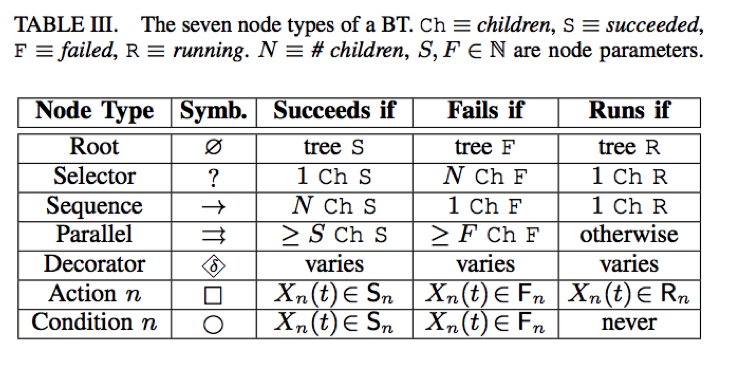
\includegraphics[width=3.25in]{Figures/BT_NODES.png}
%\caption{Different types of nodes a Behaviour Tree can have}
%\end{figure}


\begin{table}[h!]
\centering
 \begin{tabular}{||c c c c c||} 
 \hline
\textbf{Node Type} & \textbf{Symb.} & \textbf{Succeeds if} & \textbf{Fails if} & \textbf{Runs if} \\ [0.5ex] 
 \hline\hline
 Root & $\emptyset$ & tree \textit{S} & tree \textit{F} & tree \textit{R} \\ 
 \hline
 Selector & ? & 1 \textit{Ch S} & N \textit{Ch F} & 1 \textit{Ch R} \\
 \hline
 Sequence & $\longrightarrow$ & N \textit{Ch S} & 1 \textit{Ch F} & 1 \textit{Ch R}\\
 \hline
 Parallel & $\Longrightarrow$  & $\geq$ \textit{S Ch S} & $\geq$ \textit{F Ch F} & otherwise \\
 \hline
 Decorator & $\diamondsuit$ & varies & varies & varies \\ 
 \hline
  Action n & $\square$ & $X_n(t) \in$ \textbf{S}$_n$   & $X_n(t) \in$ \textbf{F}$_n$  & $X_n(t) \in$ \textbf{R}$_n$  \\
 \hline
Condition n & $\bigcirc$ & $X_n(t) \in$  \textbf{S}$_n$   & $X_n(t) \in$ \textbf{F}$_n$   & never \\
\hline
\end{tabular}
\caption{The seven node types of a BT. \textit{Ch} $\equiv$ children; \textit{S} $\equiv$ succeeded; \textit{F} $\equiv$ failed; \textit{R} $\equiv$ running; \textit{N} $\equiv$ children; $X_n(t)$ $\equiv$ current state;
\textbf{S}, \textbf{F}, \textbf{R} $\in \mathbb{N}$ are node parameters
%\patrizio{what about \textit{R} and \textit{N}?}
\cite{marzinotto2014towards}} 
\label{tab:BTnodes}
\end{table}


In a BT, each node belongs to one of the seven categories listed in Table~\ref{tab:BTnodes} taken from \cite{marzinotto2014towards}: we have one root node; leaf nodes are either Actions or Conditions, while control flow nodes are Fallbacks, Sequences, Parallels, or Decorators.
The execution of a BT starts from the root which sends ticks with a certain frequency to its child. A tick is an enabling signal that allows the execution of a child. When the execution of a node in the BT is allowed, it returns to the parent a status running if its execution has not finished yet, success if it has achieved its goal, or failure if is unable to continue with execution. A minimalistic example of a behaviour tree is presented on Figure~\ref{fig:Example}. It represents the  behaviour of the agent in the motivating scenario: an agent checks if there isn't an obstacle along its trajectory. If there isn't an obstacle, it performs a movement towards $p$.
%condition x is satisfied, behaviour plan 1 should be executed.
%When a behaviour plan 1 successfully finished,  behaviour plan 2 should start its execution. When behaviour plan 2 successfully executed, we start executing behaviour plan 3. 
If the agent successfully executed the movement towards point $p$, the behaviour tree would return success. If the agent did not reach the point $p$, the behaviour unit describing that behaviour plan returns failure which will be propagated to the root. In this case, an \textit{adaptation}  is needed.
%will be performed.

\begin{figure}[h]
\begin{center}
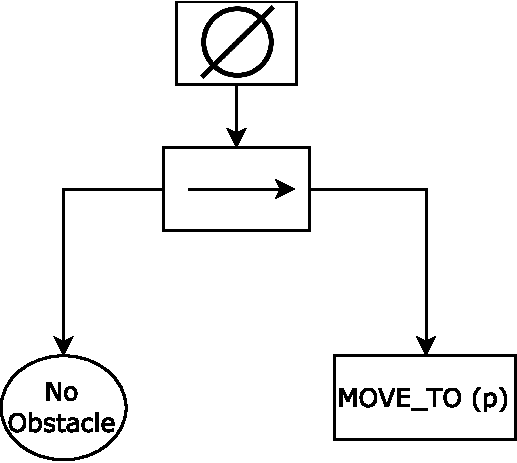
\includegraphics[width=1.85in]{Figures/BP2.pdf}
\caption{Behaviour plan for an agent }\label{fig:Example}
\end{center}
\end{figure}














%\patrizio{I don't understand the relation between goal and task. Is G=T?}
%A \textbf{Task} $T_i$ is defined by a \patrizio{why GOAL instead of goal? Please be coherent all around} GOAL space\patrizio{what's a goal space?} $G$. $T_i= G$.



%For each lower-level goal $G_i$ we associate a behaviour Bi.

%A \textbf{Behaviour} is a tuple $B_i$ = ($S_i$, $ \Sigma $,  $s_{0}$, $\delta $, $CONTEXT$, $G_i$, $r$)  where: 
%\begin{itemize}
%\item $S_i$ is a finite, non-empty set of states;
%\item $ \Sigma $ is a finite, non-empty set of transitions of Behaviour properties values that define the key characteristics of a Behaviour execution;
%\item $s_{0}$ is an initial state, \chg{ an element of S}{with $s_0 \in S$}
%\item  $\delta $ is a deterministic state-transition function:  
%$\delta :S\times \Sigma \rightarrow S $;
%\item $CONTEXT$ is a set of \textbf{Behaviour properties values} that capture the key characteristics of a Behaviour and should be valid during all the time for successful execution of a Behaviour;
%\item $G_i$ is discrete lower-level Goal that will be reached if the Behaviour is executed correctly;
%\end{itemize}

%\textbf{Behaviour} is one of the basic concepts around which we define our framework. It is  a  concept  which  explains  what  a  single agent in the system should do, without details on how the agent performs the behaviour. It's a modular, parametric, reusable structure that can be used across missions,projects and organizations. 



%It is represented by a particular MMRSs system that need to execute a set of TASKS.



%We say an agent performs a \textbf{correct behaviour} if it's executing correctly its Behaviour Plan $BP$. 

%When a behaviour reaches the \textit{success} region, we say that an agent $a_i$ completed executing its behaviour plan $BP$.
%We say that the agent is not performing a \textbf{correct behaviour} if its behaviour reaches the failure region. 


\section{Framework for mission execution}
%\patrizio{recall what the problem is. It would be nice to have a more significant name of this section.}

Missions are specified at design-time by in-the-field operators. The operators are users that are non-expert in ICT, but have specific expertise in the mission domain (like  fire fighters, policemen etc.). Within the panorama of missions~\cite{skrzypietz2012unmanned}, typical mission scenarios concern: (i) Disaster Prevention and Management, like damage
assessment after earthquakes, searching for survivors after
airplane accidents and disasters; (ii) Homeland Security, such
as coastal surveillance, securing large public events; (iii) Protection
of Critical Infrastructure, such as monitoring oil and
gas pipelines, protecting maritime transportation from piracy,
observing traffic flows; (iv) Communications, like broadband
communication, telecommunication relays; (v) Environmental
Protection, such as pollution emission, protection of water
resources etc. 
%\patrizio{I am not sure this is the right place for this text. Here we should be direct to the point, direct to the solution}
This spectrum of mission requires 
MMRSs that are both mission-critical and safety-critical systems. The definition of missions at design-time include only the information that is available at that time. 

However, a proper management of the run-time phase is required since environments in which these systems have to
operate are often unpredictable and unknown. A new plan for adaptation should be computed on the fly every time an unexpected system or environmental
feature is observed. 
However, there are few major challenges in performing adaptation on-the-fly, i.e., computing agents' behaviours on-the-fly. One challenge is to deal with the question of which part of the system should be engaged in an adaptation. This is not trivial at all, since solutions for the same problem
may be generated at different levels. For instance, an issue of
a robot (i.e., a drop of the battery level of a UAV below a
safety threshold) can be resolved in the scope of its mission,
by re-calculating its navigation plan (isolated adaptation), or in the wider scope
with the engagement of other robots and supporting systems
(e.g., a UAV trajectory manager) (collective adaptation). The challenge here is to
understand these levels and create a mechanism, which decides the right scope for an adaptation for a given issue.
The other challenge is to understand how  multiple
entities in a collective adaptation can adapt altogether and transactionally and what type of negotiation must take place to decide the right behavioural changes that should be applied on each side.
Moreover, managing the execution of complex missions requires a clear separation of concerns between safety and mission issues. This  way an operator can focus on the mission functional specification, while a safety engineer can only focus on safety-specific mechanisms that are
generic and independent from the functional behaviour of the system. 

%can be activated during mission 

%In this paper we focus on the run-time phase.

%That means that during mission execution, MMRSs have two global operational objectives which are orthogonal to each other: 
%\begin{itemize}
%\item \textbf{Safety preservation of system and environment\patrizio{this sentence is not so clear}} 
%\item \textbf{Mission completion} 
%\end{itemize} 
%These OBJECTIVES\patrizio{why OBJECTIVES?} %are prioritized meaning that safety appropriately defined should be ensured in all times, even if mission completion fails.

%employing iterative approaches in adaptation. One challenge is to compute satisfying behaviours quickly. The other
%challenge is to deal with the question of what to do when the
%specification becomes unsatisfiable due to the discovery of an
%unexpected obstacle. C

\begin{figure}[h]
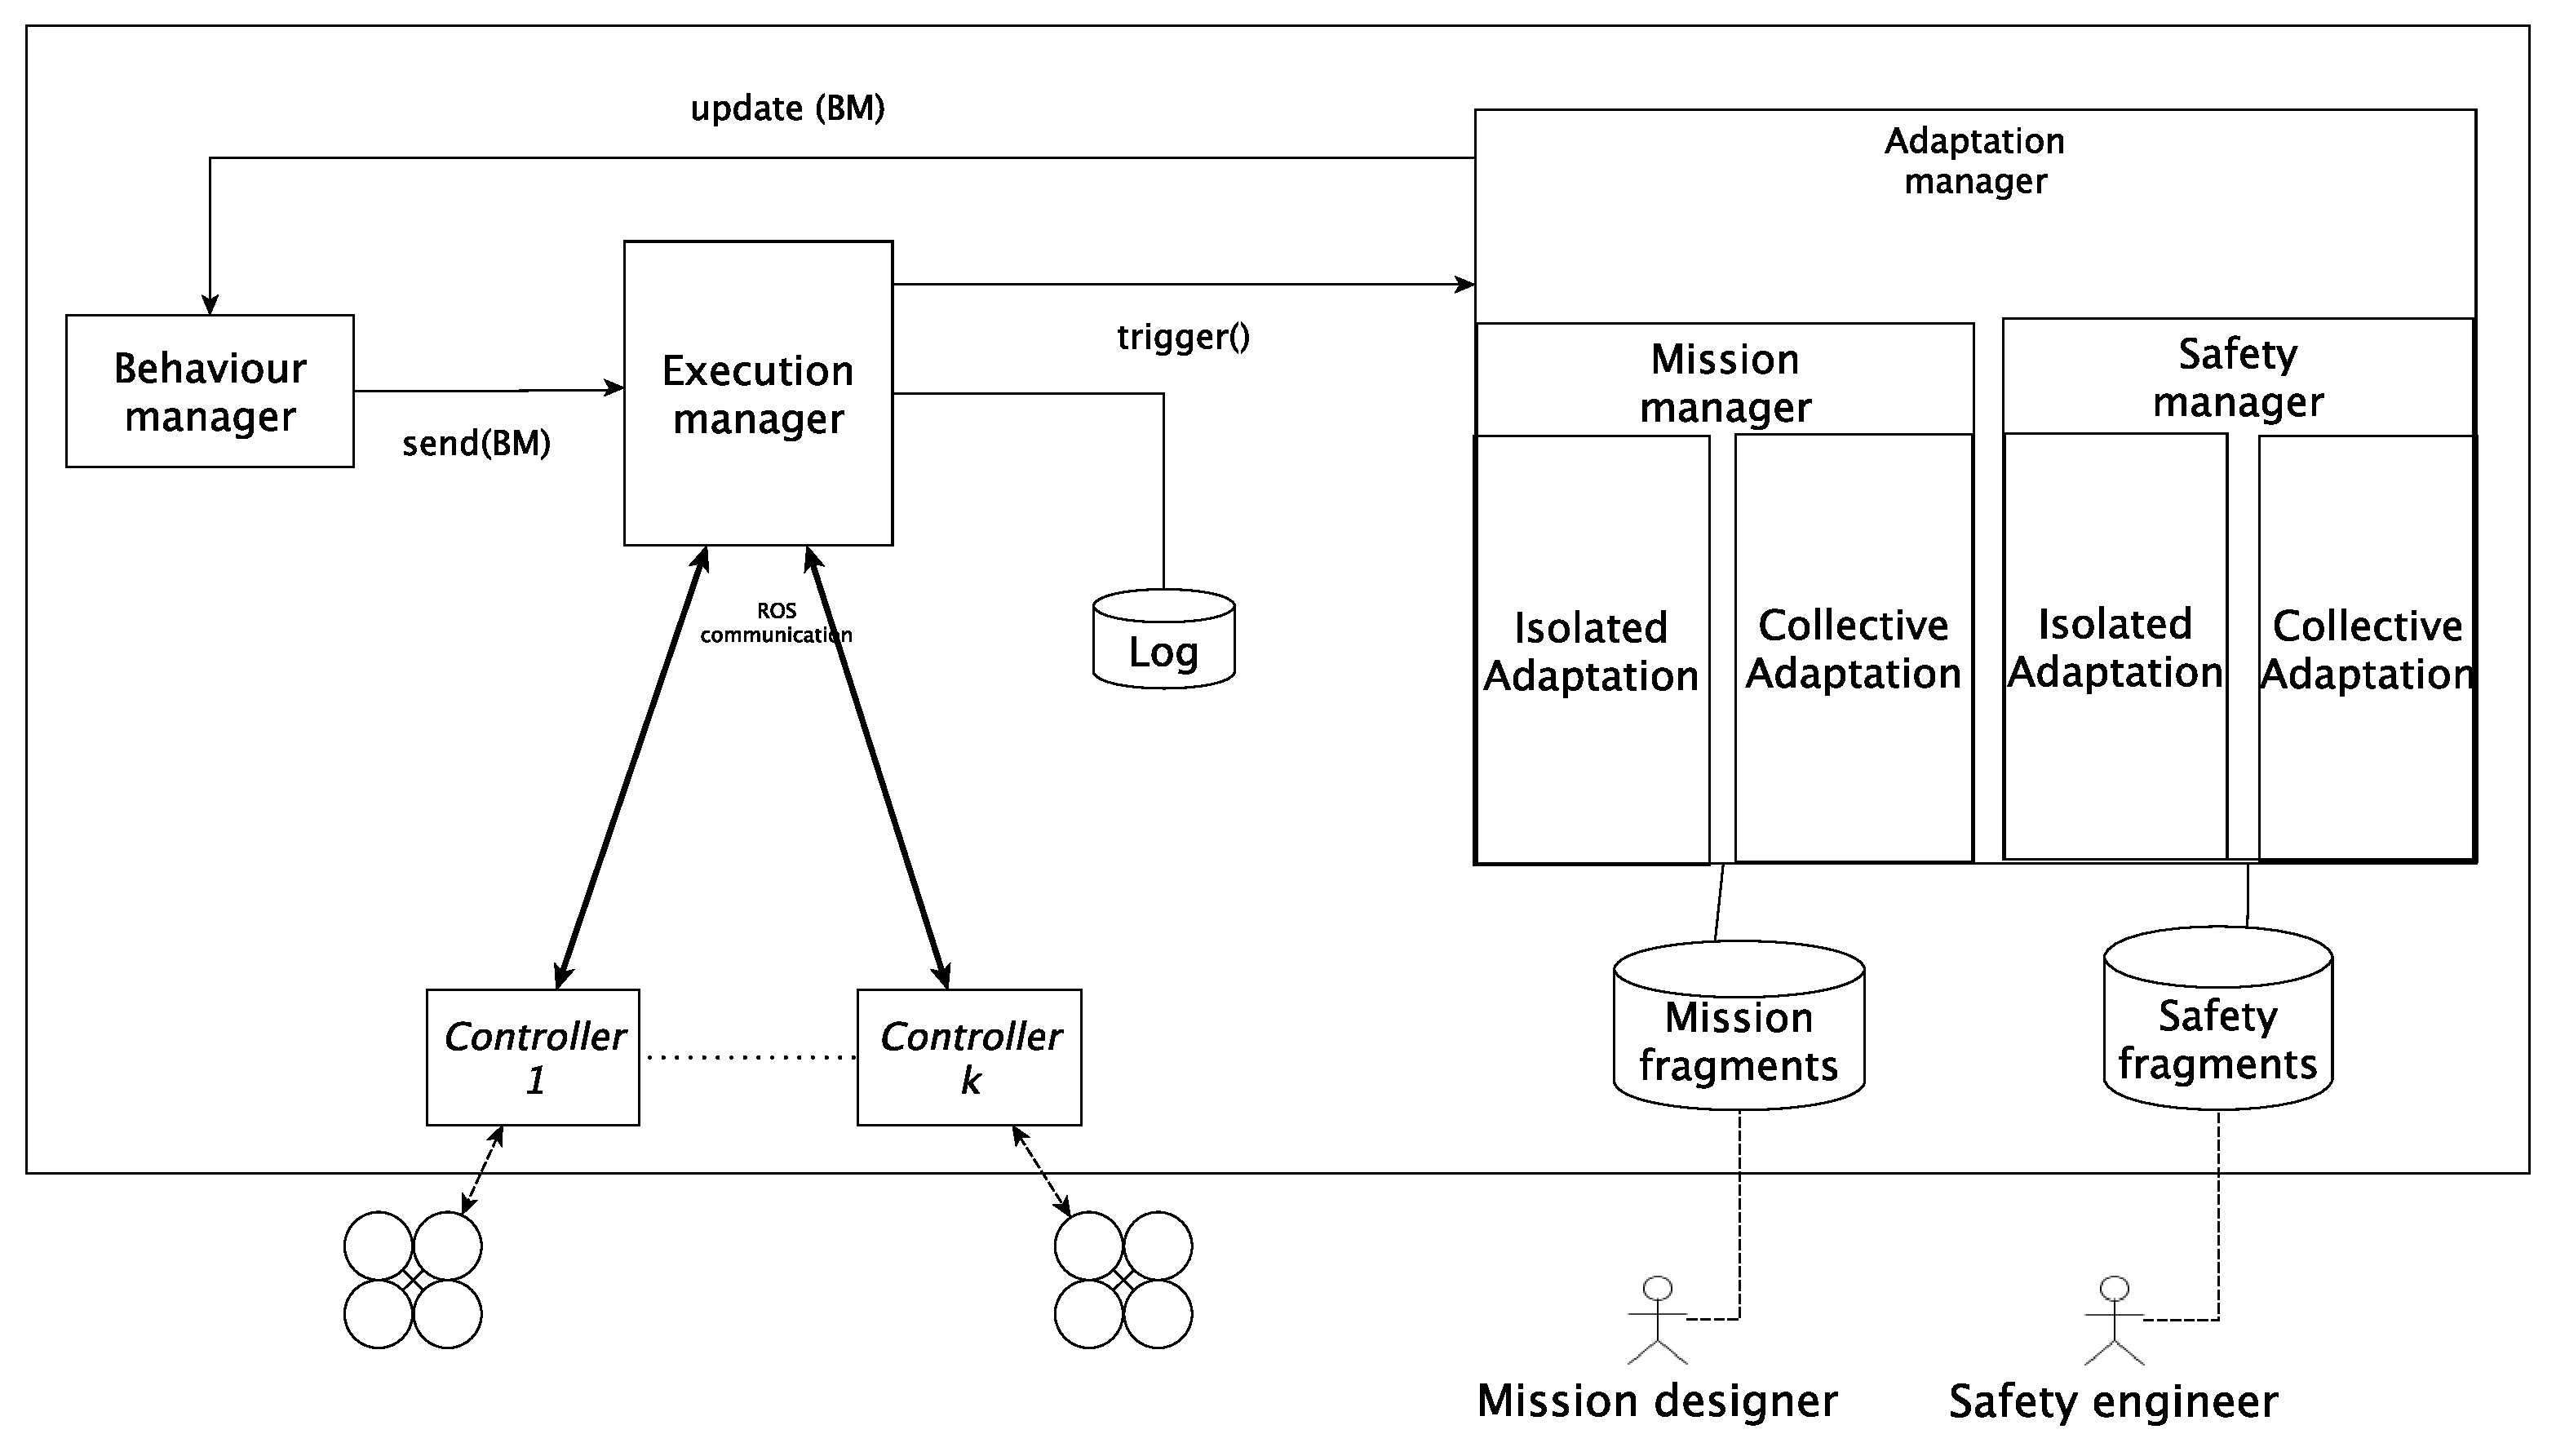
\includegraphics[width=.5\textwidth]{Figures/overall_final.pdf}
\caption{Overview of the execution framework}\label{overall}
\end{figure}


%\vspace{-.1cm}
%\begin{figure*}[ht!]
%\centering
%\captionsetup{justification=centering}
%\subfigure[Mission Execution Framework]{%
 %           \label{fig:second}
 %           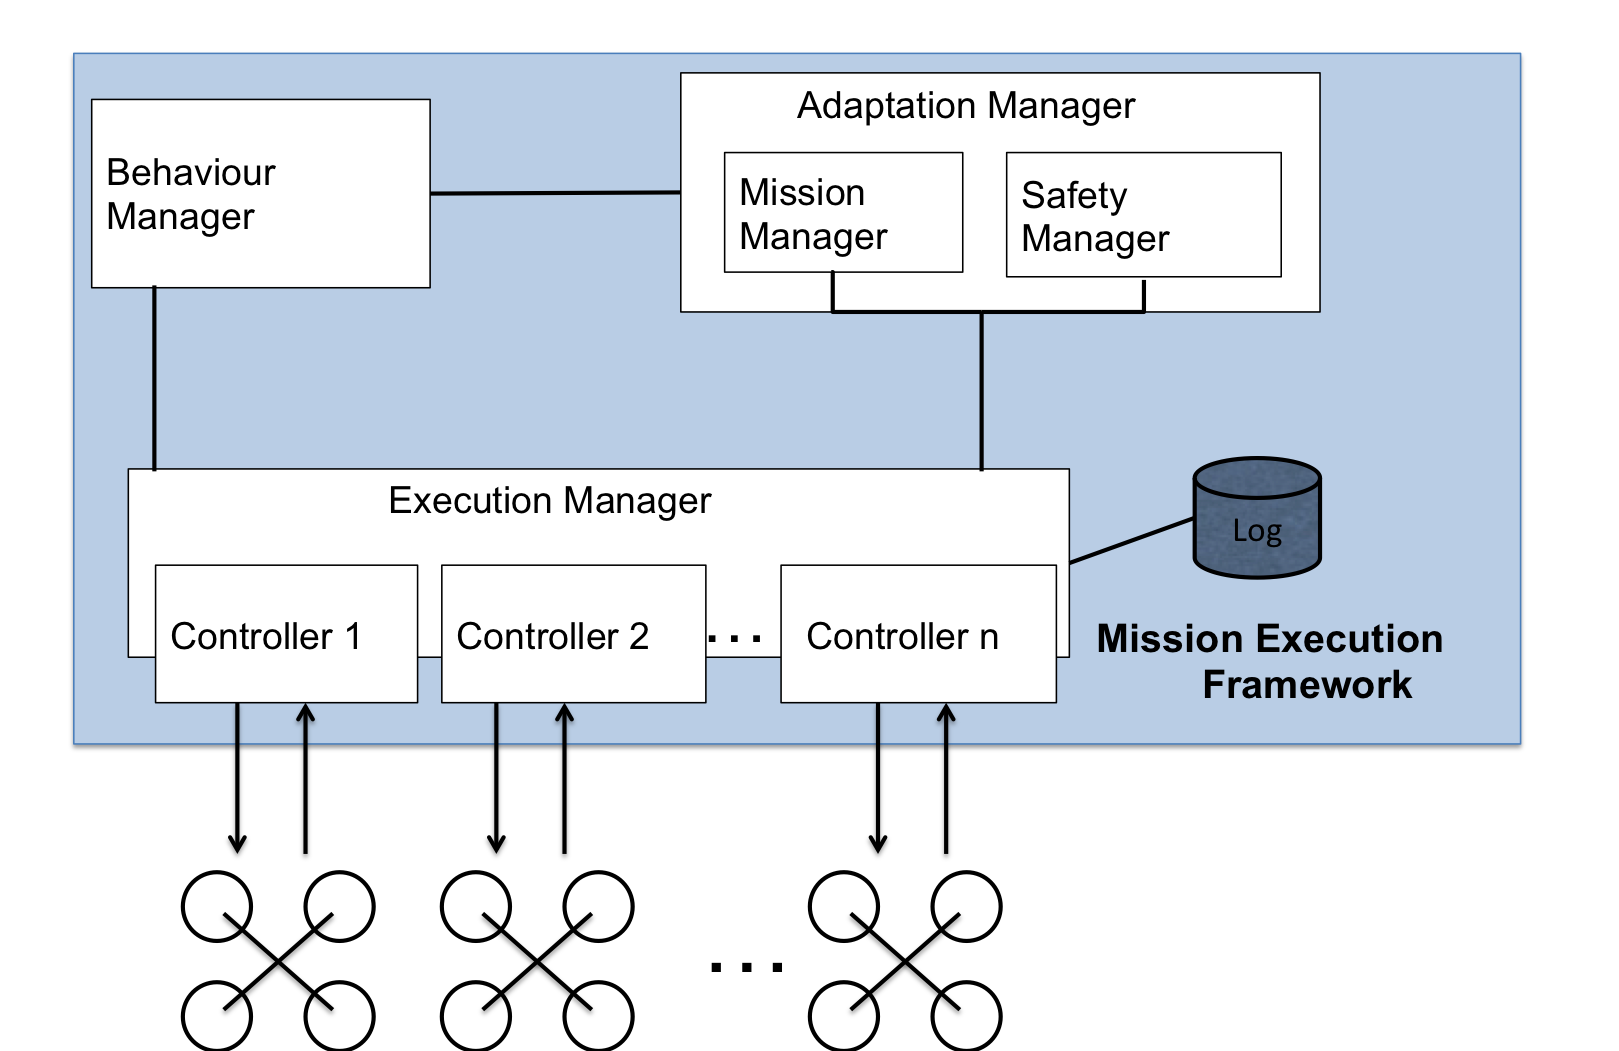
\includegraphics[width=.395\textwidth]{Figures/MissionExecution.png}
 %       }
 %       \subfigure[Adaptation Manager]{%
%           \label{fig:third}
%           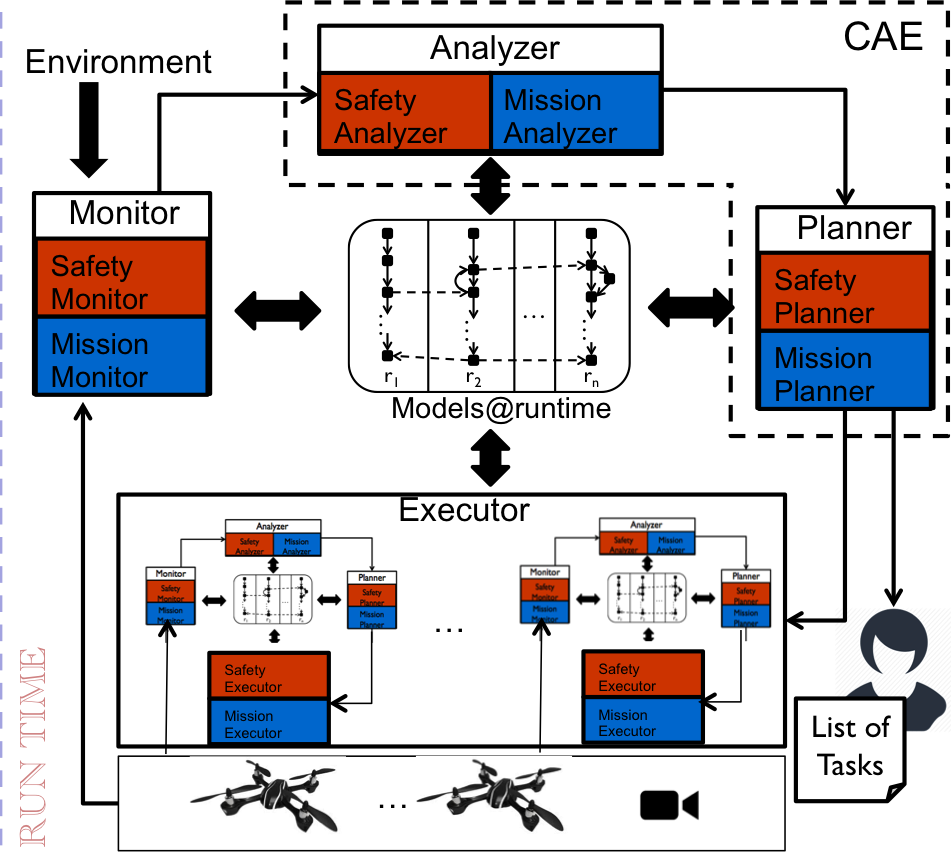
\includegraphics[ width=.35\textwidth]{Figures/Execution_Framework.png}
 %       }
%\vspace{-.2cm}
% \caption{Overview of the proposed approach\patrizio{where this figure is referenced and explained? I was expecting a figure that refers to the two algorithms mentioned in the section showing what these algorithms take as input, how these algorithms work together, etc.}}
% \vspace{-.2cm}
%\label{overall1} 
%\end{figure*}




In this work we propose a framework for supporting \textbf{execution} of MMRSs missions. A possible design-time phase for our execution framework can build on top of
the FLYAQ~\cite{bozhinoski2015flyaq, di2013engineering} platform for the specification of missions of autonomous multicopters through a high-level and graphical domain specific language tailored to the specific application
domains. In FLYAQ~\cite{bozhinoski2015flyaq, di2013engineering} the tool generates behaviour plans at design-time for each of the robots (specific types of agents) involved in the mission. The tool associates an agent (robot) $a_i$ with a subregion $SR$ for each of the mission tasks $t$. The correctness of the algorithms employed in the FLYAQ framework regarding preserving safety is proved in~\cite{ruscio2016automatic}.

Here we focus on the run-time phase.
Most of the existing works are based on the assumptions that the environment is static and that each agent has either a global communication range (can communicate with each other agent in the system) or that each agent can obtain a full knowledge of the system and the environment at any time. These
assumptions, however, do not usually hold in real-world scenarios \cite{lahijanian2016iterative}.
In our framework, an adaptation is performed on-the-fly every time an unexpected system or environmental feature is observed in a part of the system. That being said, a new behavioural plan is computed for one or a group of agents that are affected by it. Our framework supports on-the-fly adaptation that enables MMRSs to complete the defined mission while guaranteeing the preservation of safety constraints. As shown in Figure~\ref{overall} the architecture of our framework consists of 3 main components:
\begin{itemize}
    \item \textbf{Behavior Manager:} contains the behaviour model of the mission. Here, behaviour plans are stored as behaviours in a Behaviour Tree. Each agent in system is assigned a Behaviour Tree for each task. In the beginning of the mission, the Behavior Manager contains all behaviours that should be performed for completion of the mission. During mission execution, the  behaviour trees may be updated as a result of violations in the behaviour plans to one or more agents.
    %with some safety or mission related issues.
    %conditions.
   % Each behaviour in the Behaviour Tree is associated with a specific GOAL.
    \item \textbf{Execution manager} is in charge of :(i) receiving the current behaviour model of the mission from the \textit{Behaviour Manager},
    (ii) interacting
    with the controllers both to send their part of mission to be
    executed and to receive telemetry data,
    (iii) checking when some conditions in the behaviour plans are violated in order to trigger the \textit{Adaptation Manager}, and (iii) to log mission data.
    
    %\textit{Safety Manager} which is safety-specific adaptation component, (iii) checking when mission-related conditions are violated in order to trigger the \textit{Mission Manager} to perform mission problem resolution
    \item \textbf{Adaptation Manager} is a component where the adaptation happens. 
    It receives from the \textit{Execution Manager} the conditions that are violated and
    depending on the type of conditions that are violated it triggers one of its subcomponents. If safety-related conditions are violated the \textit{Safety Manager}  is always triggered. The \textit{Safety Manager} is safety-specific adaptation component that can manage only safety-related problems. If there isn't any violation of safety-related conditions and there are mission-related conditions that are violated, the \textit{Mission Manager} is triggered in order to perform mission problem resolution.
\end{itemize}









Based on the different type of issues: mission related vs. safety related the framework proposes different adaptation mechanisms which decide the right scope  for an  %organizing the different parts of MMRSs into groups
adaptation. 
  Safety is a first class concern in our missions as robots can collaborate with humans to accomplish the mission. In this context, the system should always satisfy all safety invariants, while the mission can be partially satisfied.
  That is why distinguishing between safety-related and mission-related issues is of most importance in our framework.
 %when making run-time analysis on the behaviour of the system, so we can apply different types of adaptation solutions to different issues.
 As the nature of the mission objectives is different to the safety objectives, we propose two different adaptation resolution methods: one for partial satisfaction of mission objectives and one for full satisfaction
of safety objectives. 
 In this work, a MMRS might need 
 %In this work, the need for 
 an adaptation due to the following:
\begin{itemize}
\item the system cannot successfully complete the defined mission (mission objective);
\item agent(s) performing the current mission may physically collide (safety objective). 
\end{itemize}
 The \textit{Safety Manager} contains "safety" solvers which are algorithms that generate a behavior for collision avoidance. These are agent-specific and defined independently from mission definition. The \textit{Mission Manager} contains solvers which generate a behavior for completing parts of the mission. These are mission-specific and employed  before the start of the mission.


When designing the framework we took in consideration the following types of uncertainty that the system might face and can be a reason for adaptation:
\begin{itemize}
\item \textit{Changing Availability of resources:} The availability of resources for an agent can change over time (e.g., the battery level of a robot is less then a certain value, so the robot cannot finish a task);
\item \textit{Change of environment conditions:} The environment where the agents operate is dynamic (e.g., a dynamic obstacle appears, so a robot cannot finish a task).
\end{itemize}

Even though the agents participating in the mission are autonomous, they are able to dynamically form collaborative groups, called ensembles \cite{bucchiarone2014collective} to gain benefits that otherwise would not be possible. %
The example of such a collaborative
group is an ensemble of drones that cooperate in a carbon dioxide monitoring mission represented in the motivating scenario in Figure~\ref{fig:Scenario}. Multiple entities must follow certain rules in the ensemble and in return the ensemble offers certain
advantages with respect to having single entities working independently. Adherence to these collective
rules temporarily reduces the flexibility of collaborating entities, but has huge impact on a particular quality of the system. We can consider what happens if there is a fault on a drone and the drone can't continue with its behaviour. In this case, all the tasks that the drone did not manage to complete need to be redistributed to other entities for successful mission completion, while the faulty drone needs to adapt its behaviour plan to safely exit the mission. Another issue we can consider is a collision between drones. In that case an immediate and collective reaction by a group of drones is needed for a collision to be avoided. Here, multiple entities must adapt altogether and transactionally to perform a particular collision avoidance protocol. 
This demonstrates that in MMRSs two levels of adaptation are possible: 
\begin{itemize}
\item \textit{Isolated adaptation:} change of a single agent’s behavior with pre-defined behavior templates independently from the rest of the system;
\item \textit{Collective adaptation:} collective change of the behaviour of a set of agent's teamed up in an ensemble working towards a  particular goal.
\end{itemize}

In this work, we mostly focus on collective adaptation, even though the framework has capabilities to perform isolated adaptation by providing a simple solution to a specific issue.
The framework performs on the fly collective adaptation in a decentralized fashion in order to satisfy specific mission and safety objectives. It has mechanisms that dynamically understand  which  parts of the system  should be  selected  for adaptation and can produce a solution for a specific issue. 


%The problem resolution can be performed either by one or
%multiple agents. When multiple agents participate in the mission problem
%resolution we consider their collective behavior. In order to explain
%our problem resolution process, we start introducing the notions of
%entity and ensemble. Entities are basic building blocks representing the
%different agents of the system. Ensembles facilitate cooperation of
%entities by means of an information exchange at run-time.


 
%that in adaptive systems with collective
%behavior new approaches to adaptation are needed: 1) multiple
%entities must adapt altogether and transactionally and
%2) some kind of negotiation must take place to decide on the
%changes to be applied on each side.
%
Finally, the framework is designed around the following principles:
\begin{itemize}
\item reusable, modular behaviour templates
%around which we define our framework
\item separation of concerns between mission-related vs. safety-related issues
\item for each issue type we have two types of adaptation: isolated vs. collective adaptation 
%built around the concept of dynamic ensemble
\end{itemize}
In the following sections, 
%we will introduce each principle in more details.
%In the following sections 
we will describe 
%the structure of the execution framework, 
how we model the modular reusable behaviours and how agents adapt 
when facing with mission and safety-critical issues.
%We use two different adaptation strategies to solve the different types of issues.
%\ivano{Minor: I was expecting a paragraph for each of the points above.}
%the different components that illustrate the framework. 





%Now, we formally define mission execution.
 %\begin{definition}[Mission Configuration] \darko{merge the both defitnitions} A mission configuration  ME=(C, M, S) is a tuple
%where C is the context, M is the mission that should be performed and S is the MMRS system performing it.
%\end{definition}


%\section{Execution Framework}




%Then is when adaptation should be performed. 
%In the following sections we will describe  a motivation scenario and two different types of adaptation strategies depending on the type of problems the system is facing.



%a PROBLEM CASE is generated.

%A Problem Case is a tuple Pi = (CP, f), where \begin{itemize}
%\item CP is a set of Agent's context properties that violate the Behaviour Context
%\item  $f: CP ->  V$ is function that assigns values for the different context properties.
%\end{itemize}


%Problems correspond to different critical situations that can happen to an agent when executing a particular behaviour plan. 




%Each Problem Case includes a set of parameters describing it. 

%The PROBLEM CASE is always produced by the agent that has SET OF PROPERTIES that violate its behaviour context. 

%At runtime, there is a constant check if the Agent context model satisfies the required  behaviour context values. If it doesn't, a PROBLEM CASE is generated. 
%This asks for an adaptation process to be performed.









%Solver is a tuple Si=(Pre, Pi, Bi, G) where
%\begin{itemize}
%\item Pre are the initial preconditions that should be satisfied for a Solver to be activated
%\item Pi is the Problem Case the solver will solve
%\item Bi is the Behaviour that will be generated to solve the %Problem Pi
%\item G is the Goal that will be reached after correct execution of the Behaviour Bi
%\end{itemize}

%Solver is a logical concept(algorithm, protocol) that can be activated by an AGENT to produce a behaviour that will align the Agent context model to the corresponding Behavioural context  i.e. will produce a behaviour that is a solution to an appropriate PROBLEM CASE.





%\darko{1. problem on part of the system, e.g., fault on a sensor of a drone 
%2. change on the environment, e.g. a movable obstacle is added to the environment or just move
%3. change on the mission}

%We say that a behaviour is correctly executed if it follows its specification, meaning its CONTEXT is always satisfied, until the Behaviour reaches a SUCCESS STATE.


%At runtime, there is a constant check if the Agent context model satisfies what is required in the BEHAVIOUR CONTEXT. If the Agent context model does not satisfy what is required in the BEHAVIOUR CONTEXT, a PROBLEM CASE is generated. This asks for an adaptation process to be performed.

%PROBLEM CASE correspond to different critical situations that can happen to an entity when executing a Behaviour. It is generated as a result of the inadequacy between the Agent context model and the Behaviour Context. Each Problem Case includes a set of parameters describing it. 

%The PROBLEM CASE is always produced by the agent that has SET OF PROPERTIES that violate its behaviour context. 
\section{Modeling modular behaviours}




%\patrizio{We need a running example. Introduced here so the reader will understand what we mean by mission, and then of goal, task, problem, resolution, etc.}




%\patrizio{what do you want to write in this section? Implementation aspects should be explained later, not here.}





In FLYAQ~\cite{bozhinoski2015flyaq, di2013engineering}, at design-time safe behaviour plans are generated for the agents involved in the mission  according to the initial set of active agents and the mission specification. 
%For our specific mission scenarios, we use the algorithms employed in the FLYAQ platform to generate behaviour plans for the different agents. 
Our assumption is that the algorithms used by mission designers at design-time to generate behaviour plans for the agents in our framework is correct as in FLYAQ. 
Now, we focus on the run-time phase.
During mission execution, at each point of time the system can follow the state of the mission. We define a mission state as follows.

\begin{definition}
A \textbf{Mission State} is a tuple $MS = ( C, M, S, \tau  )$ where: $C$ is the context, $M$ is the mission that should be performed and $S$ is the MMRS system performing it at time $\tau$.
\end{definition}

Furthermore, we focus on the execution of behaviour plans.
For each agent $a_i \in A$ involved in a specific task $t$ we generate a  behaviour plan $BP^t_i$. 
%If the Behaviours are executed as specified and if the execution is correct.
We define an execution of a behaviour plan for an agent $a_i$ as follows.

\begin{definition}[Executing a Behaviour Plan]
%\ivano{What is the $i$ about here? If it is relevant, then it should be also in all the elements of the tuple. In the subsequent definition, all the elements depending on $\tau$ should have it either as subscript or superscript. I think that $\tau$ should be a superscript of $EBP_i$}
We define an \textit{execution of a Behaviour Plan} for an agent $a_i$ at time $\tau$ as a tuple $EBP^i_\tau=(BP^i_\tau, S^i_\tau,  R_\tau)$ where: 
%\patrizio{if $BP_i$ is connected to the agent $a_i$ then you don't need to have $a_i$ as element of the tuple of $E$. Also, if you refer to an agent as $a_i$ then be coherent and don't use $A_i$} 
\begin{itemize} 
%\item $A_i$ is the agent that performs the behaviour plan
\item $BP^i_\tau$ is the behaviour plan performed by $a_i$ at time $\tau$
\item $S^i_\tau$ is the state of the agent $a_i$ at time $\tau$ 
%executing the behaviour plan %$a_i$
%\item PRIORITY is a dynamic numeric value that shows the importance with which an AGENT should perform the particular Behavior Bi at time t;  
%\item q is a dynamic numeric value that gives information about the quality on how well a particular agent Ai performs a particular behaviour Bi in a particular configuration Ci;
%\item $\tau$ is a particular point of time 
\item $R_\tau$ : is the return status of the Behaviour Plan ${R, S, F}$ at time $\tau$, and can be equal to either Running (R), Success (S), or Failure (F).
\end{itemize}
\end{definition}


The behaviour state space $B_i$ for an agent is partitioned in three partitions: \textit{success}, \textit{failure}, \textit{running} when an agent $a_i$ is executing a behavior plan $BP_i$ (Figure~\ref{fig:BS}). The return status of the Behaviour Plan ${R, S, F}$ at time $\tau$ describes in which partition an agent's state is. The states defined in the \textit{success} partition describe that the agent successfully completed its behavior plan. 
The states defined in the \textit{running} partition describe that the agent $a_i$ correctly executes its behavior plan at time $\tau$. We say that an agent $a_i$ is correctly executing a Behaviour plan $BP_i$ at time $\tau$ if from the current state $S_l$ the agent can continue performing its Behaviour Plan i.e., the set of conditions for the current operation $op \in BP_i$ are satisfied. %capture the configuration properties
The states defined in the \textit{failure} partition describe that the behavior plan is failing at time $\tau$. In that point the agent should adapt i.e. change its behaviour plan, so it reaches a state in the \textit{running} region from which it can continue executing the mission or just safely exit the mission as described in~\cite{di2013engineering}. In Figure~\ref{fig:BS} is represented the behaviour state space $B_i$ for an agent $a_i$ executing a behavior plan $BP_i$. The \textit{behavioural plan execution state transition} ($a \rightarrow b \rightarrow c \rightarrow d$) represents a state transition for the agent from an initial state  $S_0$ to a state in the success region $S_7$. That is only one possible state transition that could happen. There are many other possible transitions which might include the agent transitioning into a state from the failure region from where it should adapt.
%its behavioural plan to transit to a state in the running region.




\begin{figure}[h]
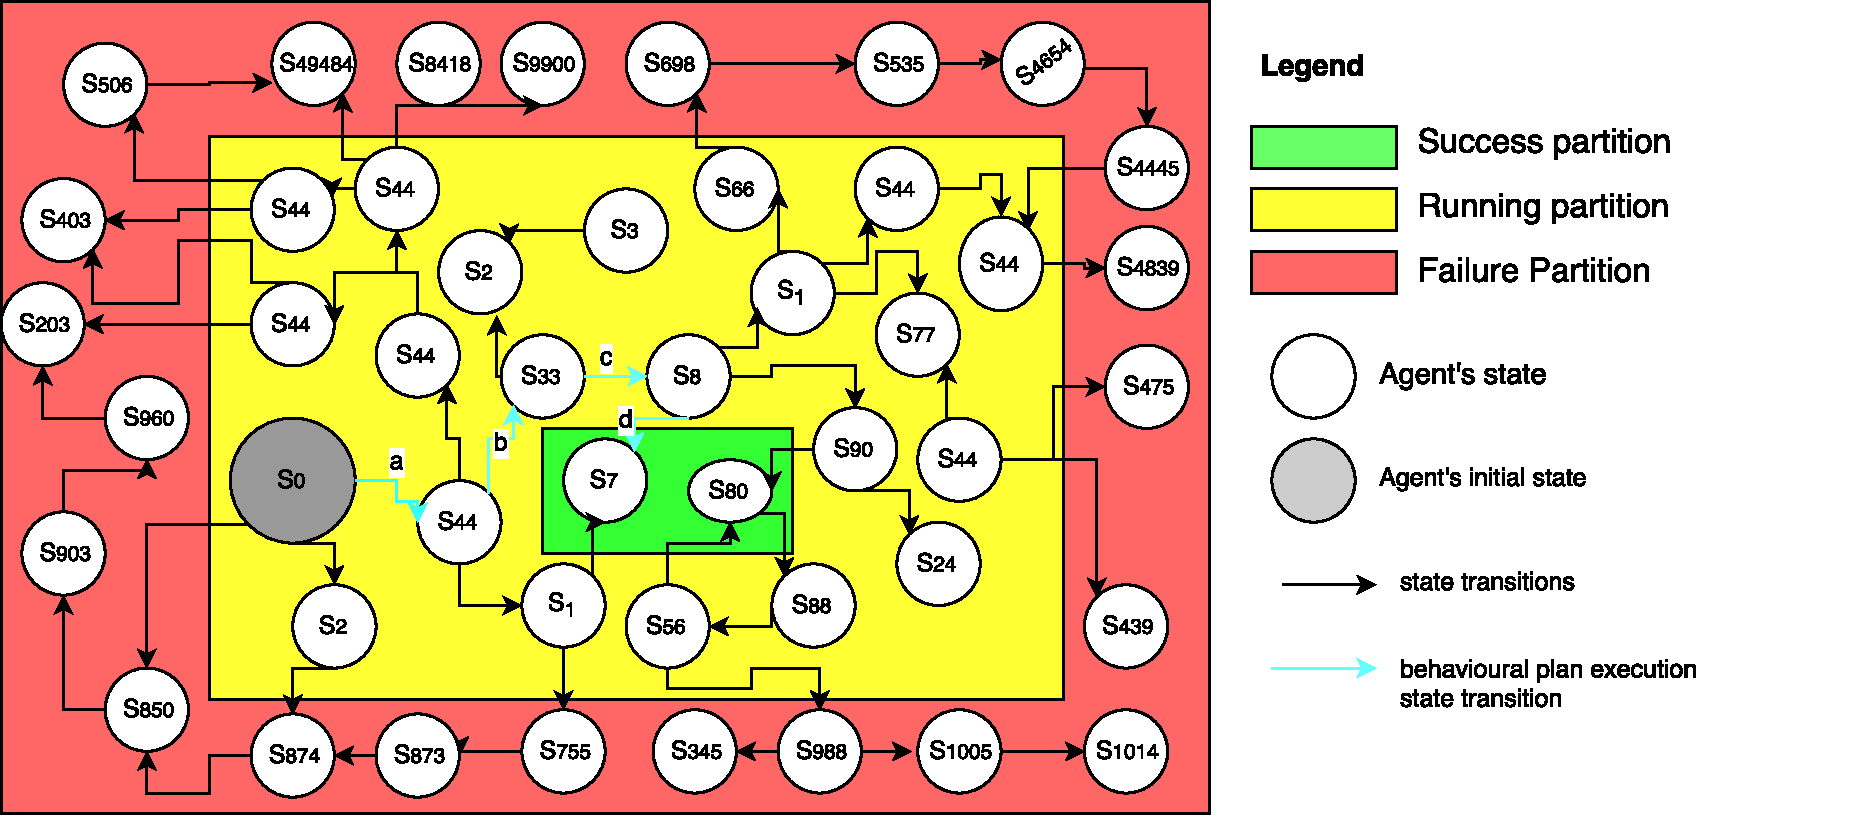
\includegraphics[width=.5\textwidth]{Figures/BS5.pdf}
\caption{Partitioning behaviour state space}\label{fig:BS}
%\patrizio{explain better the figure. also states S903 and S960 are disconnected; are these states reachable? What's the meaning? Finally, ``behaviour plan execution state transition'' is not clear. Explain better.}
\end{figure}





%\patrizio{I am missing the connection between Flyaq ans behviour trees. Are you thinking to substitute the behaviour model of FlyAQ with behaviour trees?}
To model the behaviour plans of an agent $a_i$ we will be using the Behaviour Tree Architecture because it provides a flexible mechanism for an agent to switch between different behaviour plans.
As we mentioned earlier, Behaviour Tree (BT) is an organizational execution structure that groups behaviour units that one agent should execute as part of its mission. 
Each behaviour plan of an agent is modeled as a separate behavioural unit.
 A \textit{Behaviour unit} is one of the basic concepts around which we define our framework. It's an executing structure for explaining what a single agent in the system should do as part of a task. A behavioural unit is modular, parametric structure that can be used across missions, projects, and organizations.
We believe that modularity is important when designing, testing, and reusing complex task behaviour in robotics. Individual behaviour units allow individual
behavior plans to be easily reused by other robots in other context, without the need to specify how they relate to the whole mission behavior~\cite{colledanchise2017behavior}. %Behaviour Trees (BTs) were developed in the computer gaming industry, as a tool to increase modularity in
%the control structures of in-game opponents \cite{colledanchise2017behavior} and many works propose their usage in robotic systems as well.






 








%We associate a set of active agents to perform a mission. Each agent performs a specific behaviour as part of the mission.





%\section{Modeling Mission in MMRSs}

%Mission is a list of tasks T that need to be executed.

%The state of a mission is a global state which contains the states of each of the individual tasks. 
%We document the execution progress of each of the individual tasks to determine satisfaction of the mission’s objectives.

%We specify missions as a coverage of set of GOALS(take 10 pictures in region A, take 20 pictures in region B ...).
%Mission is fully completed if all GOALS are fully completed.
%If we have partial satisfaction of some of GOALSs, we speak about partial mission completion.
%We defined the concept of a TASK in section x as a coverage of set of GOALs. space that should be reached.

%For each task 




%A key challenge in task allocation, however, is
%managing the tradeoff between leveraging pre-deployment
%plans and reacting to dynamic deviations that occur at runtime.
%Leveraging pre-deployment plans is practical and efficient, as
%aircraft operators are typically unlikely to deviate significantly
%from the flight plan that most effectively serves their mission
%in order to satisfy the needs of others.




\section{Mission and Safety Problem Resolution}
\patrizio{better using a more clear title. What's problem?}\darko{is it more clear?}

 In this section, we will discuss how our framework manages mission and safety issues. We present an iterative collective adaptation resolution method for partial satisfaction of mission objectives and full satisfaction of safety objectives. 
 
 %We discuss how the Mission Manager component resolves violation of mission-related conditions.
 
 %In order to explain our mission problem resolution approach, we first specify what a mission is.
 %A mission is represented as a coverage of set of GOALS(take 10 pictures in region A, take 20 pictures in region B ...).
 %We say that a mission is fully completed if all GOALS are fully completed.
 %If we have partial satisfaction of some of GOALSs, we speak about partial mission completion.
%We defined the concept of a TASK in section x as a coverage of set of GOALs. space that should be reached.

%For each task 
%A set of active agents performs a specific behaviour 
%We associate a set of active agents to perform a mission.
%Each agent performs a specific behaviour that is . 

During normal conditions, each agent will perform its behaviours generated at design-time and finish its part of the mission, leading to full mission completion.

 
 %A \textbf{Behaviour} is a tuple Bi = (Si, $ \Sigma $,  $s_{0}$, $\delta $, CONTEXT, Gi, r)  where: 
%\begin{itemize}
%\item Si is a finite, non-empty set of states;
%\item $ \Sigma $ is a finite, non-empty set of transitions of Behaviour properties values that define the key characteristics of a Behaviour execution;
%\item $s_{0}$ is an initial state, an element of S
%\item  $\delta $ is a deterministic state-transition function:  
%$\delta :S\times \Sigma \rightarrow S $;
%\item CONTEXT is a set of \textbf{Behaviour properties values} that capture the key characteristics of a Behaviour and should be valid during all the time for successful execution of a Behaviour;
%\item Gi is the Goal that will be reached if the Behaviour is executed correctly;
%\end{itemize}


%It is represented by a particular MMRSs system that need to execute a set of TASKS.



%We define an \textbf{execution of a Behaviour} as a tuple E=(Ai, Bi, Ci, Priority, q, t, ri) where:
%\begin{itemize}
%\item Ai is the agent that performs the behaviour
%\item Bi is the behaviour performed
%\item Ci is the current configuration of the agent Ai
%\item PRIORITY is a numeric value that shows the importance with which an AGENT should perform the particular Behavior Bi;  
%\item q is a numeric value that gives information about the quality on how well a particular agent Ai can perform a particular behaviour Bi in a particular configuration Ci;
%\item t is a particular point of time 
%\item ri : is the return status of the Behaviour ${R, S, F}$ at time t, and can be equal to either Running (R), Success (S), or Failure (F).
%\end{itemize}


%We separate the whole Behaviour State universe in three regions: SUCCESS, FAILURE, RUNNING. The states defined in the SUCCESS Region describe the GOAL we want a Behaviour to reach.

%A Behaviour that is executed under its Behaviour context is a \textbf{correct behaviour}.
%We say that a Behaviour is executing correctly at time t if the context model of the AGENT performing the Behaviour satisfies the Behaviour Context.
%i.e. the Behaviour is in the SUCCESS or RUNNING region.

%When a behaviour reaches the SUCCESS region its GOAL is reached.

However, when an agent executes a behaviour plan and reaches a state in the failure region, the behaviour is not executing correctly. When an agent is not ``executing correctly" a behaviour plan, a \textit{problem} is triggered.

A problem is a generic structure that corresponds to different critical situations that can happen to an agent when executing a particular behaviour plan. It is generated as a result of the inadequacy between the agent configuration model and the model of its behaviour plan. It can represent situations like a state of an agent that can't cover a particular mission region because of lack of resources or a state of an agent that represents a situation of possible collision.
%which actions should be performed for an agent to avoid collision avoidance.
We will discuss about the problem space  we are covering in more details in the next sections. Now, we define a problem formally as follows.


\begin{definition}[Problem]
A Problem is a tuple $P= (PS, f)$ where 
\begin{itemize}
\item $PS$ is a generic type of problems;
%\item $CP$ is a subset of the Agent's configuration parameters important for reaching $G$ 
\item  $f: P ->  V$ is an assignment function that assigns values for problem's properties to define the boundaries of the problem.
\end{itemize}
\end{definition}






A Solver is a structure that as input receives an instance of a problem and produces a behaviour plan that is a solution to a particular problem. Formally it is represented as:
%be written as:  Solver Type: P -> S, where P is the set of all possible Problem Cases and S is the set of all possible solutions.

\begin{definition}[Solver]
A Solver is a tuple $S=(P_0, PS, SS, \theta)$ where:
\begin{itemize}
\item $P_0$ is the initial problem that should be solved.
\item $PS$ is the set of all possible Problems the solver is able to solve
\item $SS$ is the set of all possible solutions
\item $\theta$ is a resolution function and $(P_i, B_i) \in \theta$ represents the following:
%that for each problem as input, the function  produces a behaviour plan as output:
\begin{itemize}
\item $P_i \in PS$ is the problem that is addressed;
\item $B_i \in SS$ is the  Behaviour Plan generated to solve the Problem (solution).
\end{itemize}
\end{itemize}
\end{definition}



The problem resolution can be performed by one or multiple agents. When multiple agents participate in the mission problem resolution we  consider their collective behaviour.
Existing approaches typically deal with
multi-agent adaptive systems through isolated adaptation: each agent adapts itself independently from each
other. However, in our work we consider isolated vs. collective adaptation.
%the problem is complicated by collective behavior. 
%Indeed, even though the agents are generally autonomous, they might dynamically form collaborative
%groups (ensembles) to gain benefits that otherwise would not be possible. The example of such a collaborative group is an ensemble of drones and ground stations that cooperate for the surveillance purpose as described in our motivation scenario: multiple entities must follow certain rules and in return the ensemble offers certain advantages with respect to having single entities working independently (e.g., robustness). Adherence to these collective
%rules temporarily reduces the flexibility of collaborating entities
%and has tremendous impact on how the entities adapt to dynamic changes. The isolated adaptation is not anymore effective in this point. 
%We can easily imagine what happens if there is a fault on a drone: the ensemble as a whole needs to perform some collective adaptation in order to recover the broken devices and to redistribute tasks to other entities in order to ensure the accomplishment of the mission. Even
%more serious consequences come if unexpected events will
%require an immediate and collective reaction to avoid collisions
%among drones; those collisions might compromise the
%safety of humans sharing the environment with the drones.
%This demonstrates that in adaptive systems with collective
%behavior new approaches to adaptation are needed that will: 
%\begin{itemize}
%\item enable entities to adapt altogether and transactionally
%\item enable some kind of negotiation to take place to decide on the
%changes in the behaviour model to be applied on each side.
%\end{itemize}
Run-time adaptation raises an important issue, i.e., identifying
which parts of the system should be engaged in adaptation.
This issue is not trivial at all, since a problem may be solved at different scales.

In order to explain our problem resolution process we
start introducing the notions of \textit{entity} and \textit{ensemble}.
%In the next part we will formally define all concepts we described above.
Entities are basic building blocks in the adaptation process representing the different agents of the system (e.g., robots, ground stations, etc.).
An entity can be seen as a representation of an agent that can play a \textit{role} in the problem resolution process. 
Formally, we define it as follows.

\begin{definition} [Entity] An entity $y = (a_i, r)$ is defined by an agent $a_i$ playing a role $r$.
\end{definition}

A role represents the type of collaborative interaction a particular agent can participate in. Collaboration consists in managing problems and  responding to problems raised. Formally is defined as follows.
 
\begin{definition}[Role] A Role is a tuple $R_i=(P, S)$ where:
\begin{itemize}
\item $P$ is a set of problems it can produce;
\item $S$ is a set of solvers it provides.
\end{itemize}
\end{definition}

%Problems generally correspond to different critical situations
%that can happen to an entity.

The model of an \textit{entity} is primarily determined by the ways it collaborates with other entities as part of an \textit{ensemble}.  In isolated adaptation the entity that triggered the problem is the same as the one that provides a solution, but in collective adaptation a solution is provided by other entities in the ensemble. An ensemble is primarily determined by the entities that collaborate to solve a particular problem. In isolated adaptation, the ensemble contains one entity, while in collective adaptation, the ensemble consists of multiple entities. In collective adaptation, the ensemble facilitates cooperation between entities by means of an information exchange at run-time. The collaboration between two entities is possible only if the entities can communicate between each other.
%themselves i.e. the communication range of one entity includes the location of the other one and vice versa.
%are in a are there  has strong dependence of the communication range between entities has a strong influence in their collaboration. 
Formally, an ensemble is defined as follows.

\begin{definition}
An Ensemble is a dynamic run-time structure represented as a tuple $E=(A, R, \lambda)$ where:
 \begin{itemize}
\item $A$ is a set of agents grouped together;
\item $R$ is a set of roles the agents are playing;
%\item $P_i$ is the problem case they are trying to solve
\item $\lambda: E \rightarrow R $ is an assignment function for which the agents are assigned their respective roles (entity definition).
 \end{itemize}
\end{definition}

\begin{definition}
A Problem Resolution is a tuple $R=(E_i, P_i, S_i)$ where $E_i$ is the ensemble  solving a problem $P_i$ and coming with a solution $S_i$.
\end{definition}

\subsection{Representing the MAPE-K loop structure in an entity}


%\subsection{Representing the MAPE-K loop structure in an entity}
In our approach each entity implements the
MAPE-K loop. 
%It is important to note that also humans
%(indirectly) follow the MAPE-K loop because their interaction with the rest of the system, often realized via devices, is required to follow an interaction protocol compliant with the MAPE-K loop \ivano{this sentence is not clear, it seems circular semantically.}.
%It is important to note that also humans (indirectly) follow the MAPE loop because their interaction with the rest of the system, often realized via devices (e.g., a smartphone), is required to follow an interaction protocol compliant with the MAPE-K loop.
%In one point of time only one behaviour can be ACTIVE.
%specific ACTIVE behaviour in a specific moment.
In Figure \ref{fig:agentsArchitecture} is represented a run-time perspective of the entity's MAPE-K architecture. This perspective represents how an entity manages the execution of the mission at run-time while preserving safety constraints.
In this section, we will describe each of the MAPE-K loop components for the individual entities. The MAPE-K loop comprises of 4 
components operating over a Knowledge base. In order to illustrate the separation of concerns between mission-related and safety-related mechanisms for self-adaptation,
there are two sub-components at each stage of the loop, one managing the mission, while the other the safety (Figure~\ref{fig:agentsArchitecture}). While both sub-components are running in parallel in the Monitor and Analysis to either obtain or update information about the system or the environment, only one subcomponent is running in the Planning and the Executor stage of the loop. In the decision of which component to run, safety has always a precedence over mission completion.
%\patrizio{explain better the interplay between the safety and mission part. For instance, if in the monitor part we are in the safety part, then we will keep the saftey part for the other three components? Or?}

In the \textit{Knowledge} base we define three different type of models that an entity contains. The first model is the Behaviour Tree model (BTM). The BTM contains all behaviour plans associated with the mission. Each entity has a set of behaviour plans defined at design-time, but only one behaviour plan can be \textit{active} in one point of time during mission execution (depending on its priority).
The second model is the current configuration of the entity \textit{Conf}. This model gives information about the current resources of an entity containing information like position of the robot in the map, current level of battery, etc.
The third model is a repository of the solvers it can provide i.e. \textit{Mission Solvers} and \textit{Safety Solvers}.
%and the problems it can trigger i.e. the roles it can play as part of the mission.

\textbf{Monitoring component}: This component receives stimuli from the environment and from the rest of the system (other entities in the system) and it updates the current configuration \textit{Conf} and \textit{BTM}. Then, it triggers the analysis component.
The stimuli are values associated with specific safety-related or mission-related properties. The \textit{Mission Monitor} keeps track of relevant mission-related information, while the \textit{Safety Monitor} keeps track of safety-related information. 


%The current configuration model of the entity is updated with information like battery, speed, location on map etc.



%If some stimuli are associated with a specific behaviour, it updates the KNOWLEDGE database marking behaviours as READY.
%Furthermore, this component also receives the status of the execution of the "current BT" and updates the knowledge model with its status(Running, Success, Failed). 


\textbf{Analysis component}: This component makes analysis if 
%gets information from the \textit{knowledge} component if the status of 
the \textit{active} behaviour either \textit{failed}, \textit{succeeded}, or \textit{running}. It has two sub-components Mission analyzer and Safety analyzer, both running in parallel and each making checking of the appropriate conditions (mission related vs. safety related).
%Furthermore, it checks if there is a new ``READY" behaviour which has higher priority then the current ACTIVE one. 
Depending on the analysis of the \textit{active} behaviour it does the following:
\begin{enumerate}
\item  Success: 
%It transfer the call to the higher MAPE-K loop (MAPE-K loop of the ensemble). 
It references the \textit{active} behaviour with the ``next" behaviour plan in the behaviour tree model. Then, it triggers the \textit{execution} component;
\item Failed:  it triggers the \textit{planning} component;
%It transfers the call to the higher MAPE-K loop (MAPE-K loop of the ensemble) .
%\item new READY behaviour with higher priority: It triggers the Planning component of the agent to start ADAPTATION
\item Running: it triggers the \textit{execution} component.
\end{enumerate}
 
\textbf{Planning component}: This component is triggered when the \textit{active} behaviour returns status failed. %or when there is a new READY behaviour with higher priority. 
The component starts the process of adaptation i.e. which as output generates a behaviour plan that will allow the entity to continue its mission execution or safely exit it.
The  planning component consists of two subcomponents: \textbf{Safety Planner} and \textbf{Mission Planner}.  When the planning component is triggered, first it gets information from the knowledge about the current configuration model $Conf$.  
Depending on the type of configuration conditions that are violated it triggers one subcomponent or the other. Safety has precedence over mission completion, so  if safety-related conditions are violated the \textit{Safety Planner} is always triggered. The Safety Planner is safety-specific adaptation component that manages only safety-related problems. If there isn't any violation of safety-related conditions and there are mission-related conditions that are violated, the \textit{Mission Planer} is triggered to perform mission problem resolution. 



%the Knowledge component if the status of the \textit{active} behaviour failed, succeed or running. 

More details about the problem resolution process will be provided in the next section where we discuss the two problem resolutions: mission problem resolution and safety problem resolution. Each of these resolutions enables two types of adaptation: (i) isolated adaptation: performed by the entity itself or (ii)  collective adaptation: performed by an ensemble of entities. The behaviour plan that is generated at the end of the adaptation process is updated in the BTM and then, the execution component is triggered.
%\darko{more info here}
%which we will describe in more details bellow.
%s of It does re-planning or reconfiguration of the system . 

\textbf{Executor component}: This component receives   the \textit{active} behaviour from the Behaviour Plan Model and executes(ticks) it i.e. issues commands to the entity's effectors.
When the executor component is triggered, first decides which subcomponent should be activated. Depending on which subcomponent performed the adaptation, it will activate one of the executor subcomponent correspondingly.  
If the safety planner was activated, the safety executor will be activated. If the mission planner was activated the mission executor will be activated. The mission executor performs mission-related behaviours, while the safety executor performs safety-related behaviours.


%taking it from the Knowledge component. , updates the KNOWLEDGE model with the return status of the ACTIVE BEHAVIOUR (Running, Success, Failed) and it triggers the Monitoring component.

%\patrizio{at this point I missed the part about creation of ensambles mentioned before. When this happen?}






\begin{figure}[h]
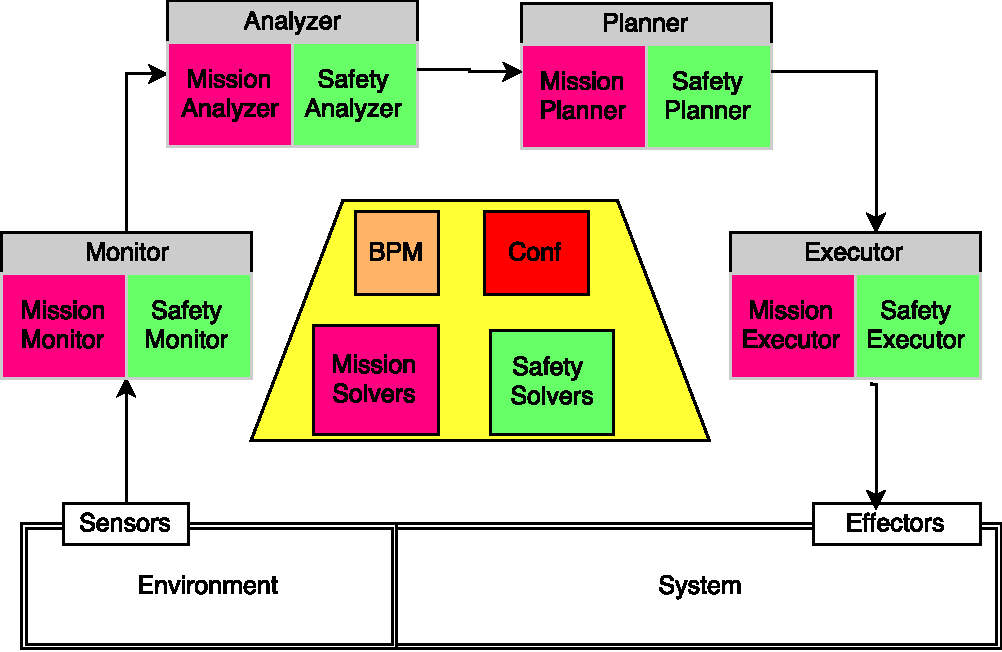
\includegraphics[width=.5\textwidth]{Figures/MAPE-K_Entity.pdf}
\caption{MAPE-K loop of an entity }\label{fig:agentsArchitecture}
\end{figure}







\section{Mission Problem Resolution}

%This definition of a solver allows partial solving of a particular problem. 
%Solver is a tuple $S_i=(piC, P, B_i, G)$ where
%\begin{itemize}
%\item $piC$ is a set of solver constraints (configuration parameters that reduces the space of acceptable Problem Cases) that should be satisfied for a Solver to be activated (ex. Agent should have an active camera as a resource etc.)
%\item $P$ is the set of all possible Problem Cases the solver is able to solve
%\item $B_i$ is the Behaviour generated to solve the Problem (solution)
%\item $G$ is the Goal space that is addressed with the generation of Behaviour $Bi$. 
%$Gi$ reduces the problem space $Pi$.
%\end{itemize}
 
 

 
 
 

 
In an initial work \cite{bozhinoski2016leveraging}, we provided a generic approach for managing run-time adaptation with general types of problems and solvers that can be triggered during mission execution.
Our framework implements a \textit{Mission Manager component} as part of the Planning component in the MAPE-K loop for each entity. 
%If the entity can perform isolated adaptation i.e. contains solvers which can generate a solution
%behavior for completing parts of the mission. These are mission-specific and employed  before the start of the mission.
 The mission manager receives information about the eligible mission related solvers in the Knowledge base. These are mission-specific and defined before the start of the mission. Mission-specific solvers have a set of solver constraints (configuration parameters) that reduce the space of acceptable problems (e.g., a solver for covering a geographical area might require an entity to have an active camera, enough level of battery etc. to be  able to resolve a particular problem).  If an entity %activate an perform isolated adaptation
 activates an eligible solver, it generates a solution i.e. behaviour plan to complete parts of the mission.
 The generated solution (behaviour plan) brings the agent into a state from which it can continue executing the mission.
%\darko{what are the consequences of behaviour plans execution}
 Here, the scope of mission specific problems is related to the nature of our definition of mission. In order to explain the \textit{mission problem resolution process}, we frame the scope of problems for isolated and collective adaptation.
 An entity might perform isolated adaptation when facing with a situation where its behaviour plan trajectory needs to pass through a no-pass zone. In this case, the entity might have a solver that generates a behaviour plan for avoiding a no-pass zone. Next, we will speak in more details about collective adaptation.

%partitioning the different types of problems and solvers and 
\subsection{Collective adaptation}
At design time we assigned the goal space $G$ for a task $t$ to a set of agents $A$. On Figure~\ref{Fig:Synthesis} the goal space $G$ is assigned to two agents $a_1$ and $a_2$. A subregion $SR^t_i$ of a task $t$ that a specific agent $a_i$  was assigned to do is decomposed in number of blocks (e.g.: the rectangle delimited by $q11$, $q16$, $q15$, and $q12$ in Figure~\ref{Fig:Synthesis} is one block).
%We showed in \cite{bozhinoski2015flyaq, di2013engineering} how we decompose the regions on blocks.  
Then, for each block we assigned a unique identifier and associate a goal location $G_i \in Coordinates$. 
For each agent $a_i \in A$ involved in a specific task $t$ we generate a  behaviour plan $BP^t_i$ covering a sub-region $SR^t_i \in G$ from its home location $G^i_{home}$ to the last goal location $G^i_n$. 
%(ex. on Figure~\ref{Fig:Synthesis} those are c1 and $G_9$ correspondingly)

\begin{figure}[h]
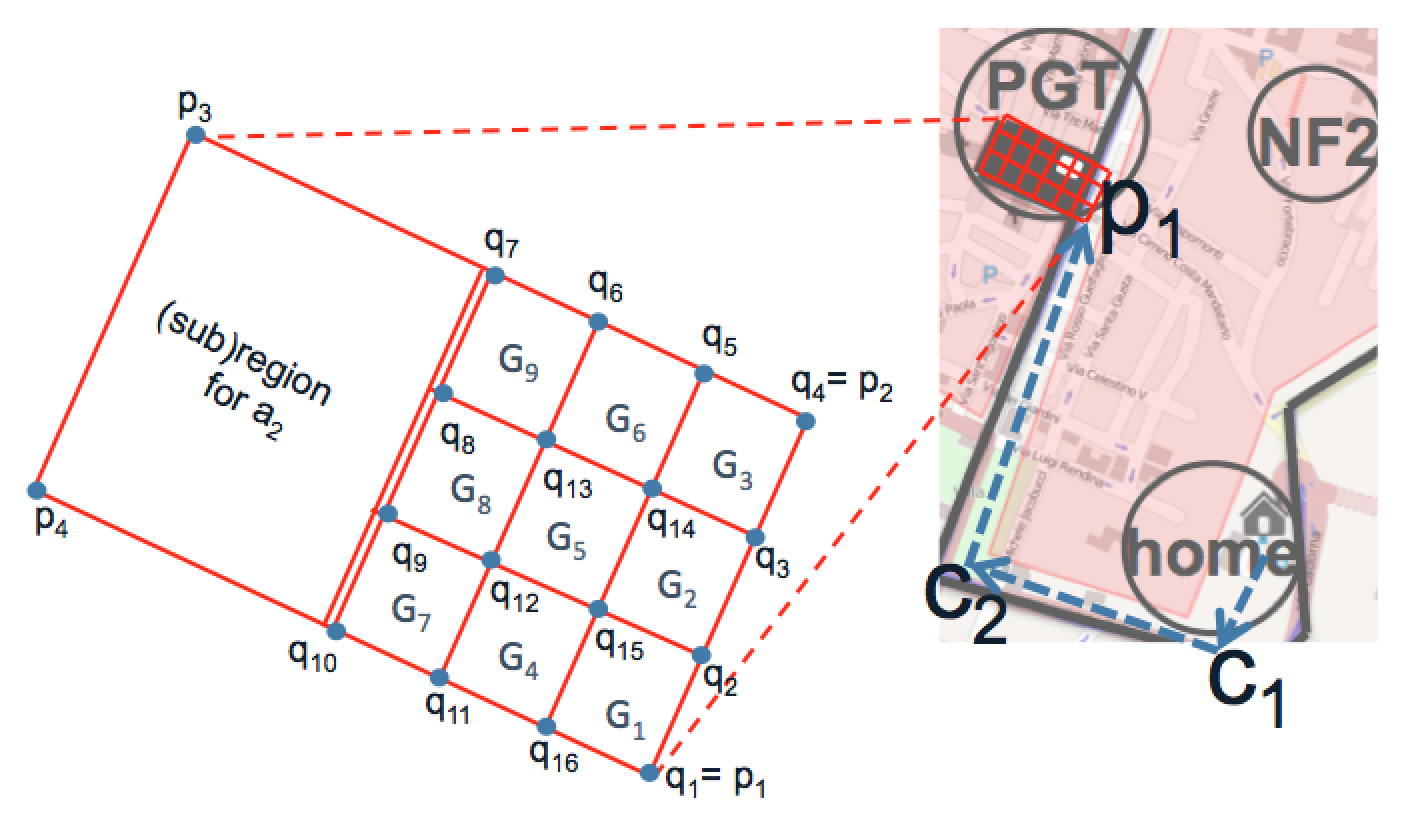
\includegraphics[width=3.25in]{Figures/Synthesis2.png}
\caption{Task assignment for two agents}\label{Fig:Synthesis}
\end{figure}



 As mission-specific problems strongly depend on the type of tasks the MMRS performs, in this context, we define a mission-specific problem as a coverage path planning problem for a set of blocks in a subregion $SR^t_i \in G$ of a task $t$ that a specific entity $y_i=(a_i,r)$  was assigned to cover, but was not able. The uncovered region is called a \textit{problem's space}.
Accordingly, we focus only on one type of mission-specific solvers which represent \textit{strategies} for covering a region. The mission-specific solvers are formulated as algorithms solving a coverage path planning problem which depends on the type of the geometry of the task $t$. Example of a solver can be an algorithm that generates a solution for covering a region with respect to a specified grid of points as in Figure~\ref{Fig:Synthesis}.

 %and here, we defined mission tasks as covering problems, in this paper  our collective adaptation based 
%coverage path planning problem. 

As we work particularly with regions, a mission related problem can be decomposed on smaller problems(sub-regions). 
To be able to annotate the progress of task execution, we define a measure of satisfiability for a task $t$ that gives information on how much percentage of the task goal space $G_t$ is covered. %\darko{more details}
We denote that a task $t$ is completed if all blocks of its goal space $G$ are covered i.e. all generated lower-level goals $G_i$ are reached. Correspondingly, we  say  that  a  mission is \textit{fully completed} if all tasks are completed. 
In contrast, a mission is partially completed if there is a task $t$ which is not completed i.e. there is a task $t$ with a subregion $SR^t_i$ that contains blocks which are not covered.
%subset of all regions' blocks are covered. 



In collective adaptation, the Mission Manager of an entity can decompose larger problems into smaller ones and can provide a partial solution to the initial problem. 
The mission manager receives information about the eligible mission related solvers in the Knowledge base and generates a solution i.e. behaviour plan. The solution is a generated behaviour plan that covers part of the problem space.
%is a solution that an entity can provide for this mission-specific problem. 
%Mission related solvers have a set of solver constraints (ex. configuration parameters) that reduce the space of acceptable problems (ex. a solver for covering a geographical area might require an entity to have an active camera, enough level of battery etc. to be  able to resolve a particular problem).
Our definition of a solver in this particular context allows partial solving of a particular problem due to the fact the problems can be decomposed into smaller ones. 
%The Mission Manager component generates a behaviour plan based on the mission related solvers (in our case behaviour strategies for decomposing an area on blocks.)
%. were looking into our approach is general,
%meaning that it is not domain or problem specific.

% and we provided a general type algorithm for problem resolution. 

%should be able to cover a part or the full region defined in the problem.
In this context, \textit{Mission problem resolution} consists in reducing the problem space of a problem until the problem space is empty or until a specific time deadline is reached. We believe that cooperation in emergent application scenarios requires a new kind of problem resolution approach which is efficient in terms of short delay, so we defined a time deadline until when a solution should be found. If a full solution to the problem is found before the deadline, the mission problem resolution process don't need to wait until the deadline is reached, but it immediately returns the found solution.
We formally define a solution of the mission problem resolution as follows.

\begin{definition}
A solution in the mission problem resolution $R$ is defined as:
$Sol=\max \limits_{ \emptyset \leq P_i \leq P_o} R(E_i, P_i, d)$
%$$MR=\lim_{P_i\to \emptyset; t \to d} f(E_i, P_i, max(S_i)))$$ 
where $E_i$ is the ensemble solving a problem $P_i$, $P_0$ is the initial problem that should be solved, $d$ is a time deadline and $Sol$ is the best solution found for that particular time deadline $d$.
%$\sum_{\substack{1 \le i \le 10 \\ 1 \le j \le 5}}^\infty x^{i} y^{j} $

%$\max\limits_{\substack{0 \leq t \leq d; \\ \emptyset \leq P_i \leq P_o}} x^i y^j$

%$\max \substack_{0 \leq t \leq d;\\ \emptyset \leq P_i \leq P_o}$

%, $\max\limits_{1 \leq j \leq n}_{1 \leq j \leq n;}$


\end{definition}

%In other words that means that the region that should be covered by a particular set of agents. 

%We believe that cooperation in emergent application scenarios requires a new kind of problem resolution approach That is why


%executed. 
 %We will explain the whole approach in more details in the next section.


%did not full all lower-level GOALS $G_i$ are achieved.


%\begin{definition}
%A Problem is a tuple $P_i= (PS, CP, f)$ where 
%\begin{itemize}
%\item $PS \in R$ is a goal space(region) of a task $t$ an agent was assigned but not able to perform. We named this particular goal space as a \textit{problem space}.
%\item $CP$ is a subset of the Agent's configuration parameters important for reaching $G$ 
%\item  $f: CP ->  V$ is an assignment function that assigns values for the agent's configuration parameters important for reaching $PS$
%\end{itemize}
%\end{definition}

%It is associated with a problem space \patrizio{what's a problem space?} that can be decomposed on smaller problems. 





%Solver is a tuple $S_i=(piC, P, B_i, G)$ where
%\begin{itemize}
%\item $piC$ is a set of solver constraints (configuration parameters that reduces the space of acceptable Problem Cases) that should be satisfied for a Solver to be activated (ex. Agent should have an active camera as a resource etc.)
%\item $P$ is the set of all possible Problem Cases the solver is able to solve
%\item $B_i$ is the Behaviour generated to solve the Problem (solution)
%\item $G$ is the Goal space that is addressed with the generation of Behaviour $Bi$. 
%$Gi$ reduces the problem space $Pi$.
%\end{itemize}
 
 
%In order to explain the model of mission problem resolution we introduce the notion of an ensemble.





 

 %\patrizio{expalin better the concept of ensamble and why we need that} 
 
 
 

%\patrizio{Resolution of what? What are we solving?} 

To specify the model of the ensemble needed for problem resolution of mission related problems in details we will be  using the declarative Ensemble
Definition Language (EDL) \cite{bures2015towards}.
The main section of the ensemble specification is
the \textit{ensemble membership} which defines the
structure of the ensemble.
A structure of an ensemble is defined through the ensemble
roles the agents can participate in. A partial EDL Specification for the mission resolution ensembles is presented on Figure~\ref{lstEDLMission}.
%\begin{lstlisting}[caption=EDL Specification for mission resolution ensembles, language=Python, label=lstEDLMission]
%ensemble MissionResolution
%    id ensemble_id: Agent
%    membership
%        roles
%           Leader : Agent
%           Solver_Agent [1..n]: Agent
%    constraints
%        constraint Agent.hascommpath(Leader)
%    fitness sum Leader.solution.quality+Solver_Agent.solution.quality
 %   knowledge exchange
  %      Agent.target = Leader.id
  %      Agent.Problemid = Leader.Problemid
%        Leader.solution=Agent.solution
%\end{lstlisting}
\lstdefinelanguage{sl} {morekeywords={ensemble, id, constraints, constraint, fitness, knowledge, exchange, membership, roles, sum, e, if, in, continue, break, else, goto, return, function, then, fi, end, foreach, defer, on, state, entry, start, machine }}
\lstset{mathescape=true, keywordstyle=\bfseries\underbar, tabsize=1, commentstyle=\itshape, numbers=left, numberstyle=\tiny, %xleftmargin=\listingnumberwidth, 
numbersep=1em}
\vspace{-0.5cm}
\begin{center}
\begin{figure}[!h]
 \lstinputlisting[language=sl, basicstyle=\scriptsize, tabsize=4,xleftmargin=3.0ex]{src/main2.src}
%\lstinputlisting[multicols=2,language=sl, tabsize=2]{src/mainAnto.src}  
\vspace{-0.2cm}
 \caption{EDL Specification for mission resolution ensembles} 
 \label {lstEDLMission}
\vspace{-0.7cm}
\end{figure} 
\end{center} 
 

%The ensemble is defined in terms of roles and role connectors. A role can be seen as a meta-component that can be instantiated by agents of different types.
%An ensemble introduces a set of roles that can be taken by participating agents, and a set of constraints regulating the operation of participating entities in the scope of ensemble.
%As such, we define a run-time agent structure named role that includes a
%set of Problem Cases it can produce, and a set of Solvers it provides.
%Role  is a dynamic run-time structure represented as a tupple Ri=(Ai, P, S) where:
%\begin{itemize}
%\item Ai is an agent
%\item P is the set of Problem Cases an Agent Ai can raise playing the role
%\item S is the set of solvers that Agent Ai can activate playing the role
%\end{itemize}
 %We specify the ensemble type used for mission problem resolution on Listing 1.
To identify the ensemble, we declare the id of the entity playing the role Leader to be the id of the ensemble – essentially
saying that instances of this ensemble type cannot be
created without being associated with a unique entity
instance, which can be seen as a sort of coordinator
of the ensemble.

The ensemble membership function 
consists of three sections. First, the
structure of the ensemble is defined by declaring the ensemble
roles that the entities can play.
In our case, an agent can play one of the following roles in the mission resolution ensemble:
\begin{itemize}
\item Leader: an entity that triggers a problem $P_k$ and leads the ensemble formation;
\item Solver\_Agent: an entity that participate in the solution creation of the aforementioned problem $P_k$.
%\_1, Solver\_Agent\_2, ... , Solver\_Agent\_N  
%(roles of agents that participate in the solution creation of the aforementioned problem)
%\item LEADER (an agent that provides a final solution to a triggered top-level problem case). In situations where the ROOT\_AGENT provides a partial solution to its triggered problem case, the agent that has the role ROOT\_AGENT has also the role ROOT LEADER ENSEMBLE
\end{itemize}
An agent can play more then one role in the ensemble i.e. it can be a leader and a solver\_agent (it can trigger a problem, but at a same time it can provide a partial solution to the problem it triggered).
%Role is a set of behaviours that an agent can "play" at run-time for execution of a TASK. The agent can play a specific role only if it satisfies the constraints c. These type of constraints usually are:  (1) information if the AGENT contains a specific resource or (2) information about the state of a resource of an AGENT. 
%(Example. The GROUND STATION (TYPE AGENT) can't play the ROLE "PHOTOGRAPHER. (1) A drone can play the ROLE "Photographer" only if it has a CAMERA. (2) A drone can play the ROLE "Photographer" only if it has "enough" battery). Roles are reusable units.
%Role is a run-time instance that 

%Role  is a dynamic run-time structure represented as a tupple Ri=(P, S) where:
%\begin{itemize}
%\item Ai is an agent performing a behaviour Bi
%\item Bi is a behaviour
%\item P is the set of Problem Cases an Agent Ai can raise playing the role
%\item S is the set of solvers that Agent Ai can activate playing the role
%\end{itemize}

%An ensemble is defined in terms of roles and role
%connectors. A role can be seen as a meta-component (or a type) that can be instantiated
%by components of different types

%an ensemble is a specification that defines how a certain type of collaboration
%occurs between several entities. An ensemble introduces a set of roles that can be taken
%by participating entities, and a set of constraints regulating the operation of participating
%entities in the scope of ensemble.

%Ensemble is a dynamic run-time structure represented as a tupple Ei=(Ai, G) where
%\begin{itemize}
%\item A is a collection of agents grouped together working
%\item G is the GOAL they are workings towards
%\end{itemize}
 
Next, we place semantic constraints, represented by the constraint expression. In our scenario a constraint for an entity to be part of the ensemble is that there must be a \textit{communication path} between the corresponding entity and its leader. What we mean by communication path is that if the ensemble leader sends a message in the environment, the information can be transferred from one entity to another, and all entities that are able to receive the information are in the communication path of the leader.
%transit and the corresponding agent is able to receive it after infinite time. all the agents that can receive that information after infinite time in the environment
In other words, each entity in the ensemble should have a neighborhood region that is overlapping with the neighborhood region 
%in its neighborhood region 
%for each entity in the ensemble overlaps 
%neighborhood region of another e
of at least one other entity from the same ensemble. Neighborhood $NR$ is a region of an entity $e_i$ that gives information with which other entities can communicate in a particular point of time $\tau$. At any point of time during mission execution, each entity in the system has partial view of the system that consists of a list of entities \textit{neighbours} that can communicate with. 
 %at that time.
%Here, we assume that all entities preserved their position in the environment (they are static for some time period $\tau$). 
%i it taking in consideration the fact that all Agents preserved their position in the environment.
The third part of the membership definition is the fitness function, specified with a numeric expression. The fitness function provides information about which aspect of the ensemble membership should be optimized. That gives the framework a way to decide which entities should participate in the ensemble formation. More precisely, ensemble instances will be created in such a way to maximize the fitness function. In our example, the fitness function is calculated as a sum of the solution quality provided by all entities in the communication range of the leader. Finally, knowledge exchange is specified, creating an information exchange between the members of the ensemble. In our case, we have exchange of three types of information. First, is the information on which entity is the leader in the ensemble (line 11), second each of the entities in the ensemble has information about the problem that should be solved (line 12) and last is the solution that the leader obtains 
%about the solution that can be provided 
for each entity in the ensemble (line 13). 

\subsection{Mission Problem Resolution Algorithm}



%Each problem includes a set of parameters describing its boundaries. Its solver provides a set of constraints describing its resolution.





% The resolution process consists of formation of an ensemble where each agent contributes towards the problem resolution with a partial solution.

We propose a best-effort approach for mission problem resolution which is efficient in terms of short delay and which does not require knowledge of which and how many entities(agents) are in the system in a particular point of time.
To realize our approach, we abstractly define a recursive best-effort algorithm that covers the procedure for mission problem resolution.
The algorithm starts from an entity $e_i$ that originally detected a Problem $P_i$ and expects to commit a solution until a time deadline $d$.
%The function is called locally by an agent $a_i$ that originally detected a Problem $P_i$ and expects to commit a solution until a time deadline $d$. 
Further recursive calls are propagated to other entities in the environment using events.
%a Remote Procedure Call.

The algorithm consists of three phases:
\begin{enumerate}
\item discover phase 
\item construct phase
\item commit phase
\end{enumerate}
 
 In the \textbf{discover phase},  %information regarding 
 %which could be the 
 the possible entities that can participate in the mission problem resolution are found. Each of the entities that can contribute with a solution to a specific problem and have a communication path towards 
 %the agent that triggered the problem
 the leader are discovered and links between each of the corresponding entities is created. 
 At any point of time during mission execution, each entity in the system has partial view of the system that consists of a list of entities \textit{neighbours} that can communicate with. Neighborhood $NR$ is a region of an entity $e_i$ that gives information with which other entities can communicate in a particular point of time $\tau$.
 %at that time.
 Each entity that contains an active solver(solver for which the preconditions for activation are fulfilled) %and can generate a solution
 can contribute towards a solution to the mission-specific problem if it is in a \textit{communication range} with the entity that triggered the problem. In the \textbf{discover phase}, those entities are found
 %resolution process is discovered 
 and a \textit{temporary} ensemble is formed. The \textit{temporary} ensemble consists of all possible entities that might participate in the resolution process.
 
 In the \textbf{construct phase}, each discovered entity in the \textit{temporary} ensemble contributes towards the global solution formation.
 Each of the entities in the communication range contributes towards the global solution by resolving a particular sub-problem of the general problem, and produces a solution with some specific quality $q$ until a specific deadline $d$ is reached. Hence, solutions are composed from multiple solvers from different entities, the same way problems can be decomposed on multiple sub-problems. In the end, the entity that triggered the problem resolution process  decides which is the \textit{best} solution and which part of the temporary ensemble contributes towards it.
 
%In the \textbf{commit phase}, the entity that triggered the problem resolution process requires a commitment from each entity that contributes towards the best solution.
%in the "temporary" ensemble. 
In the \textbf{commit phase}, the leader of the ensemble knows how well each of the entities can solve a particular sub-problem so it sends request to the entities that can contribute with the best solution to commit their resources. 
%After agents in the ensemble commit their resources for execution, a \textit{stable ensemble} is formed and the \textit{final solution} is obtained.
Meanwhile, some of the entities might leave the \textit{temporary} ensemble due to a lack of resources, because they have commitment for another problem resolution process or because they are not anymore in the neighborhood of the entity that triggered the problem.
After entities commit their resources for execution,   a \textit{stable ensemble} is formed and the \textit{final solution} is obtained.
%a \textit{final solution} is obtained. 
The ensemble that provided the final solution is called \textit{stable ensemble}. It is the ensemble that provides guarantees about the proposed solution i.e. if all behaviours from all entities in the final ensemble execute correctly (according to the generated behaviour plan), the final solution will be guaranteed.



%As described  previously, the algorithm consists of three phases:
%\begin{itemize}
%\item discover phase 
%\item construct phase
%\item commit phase
%\end{itemize}
% In the \textbf{discover phase}, the possible agents in the dynamic ensemble are found. Each of the agents that can contribute towards a solution to a specific problem and have a communication path towards 
 %the agent that triggered the problem
 %the leader are discovered and links between each of the corresponding agents is created. \\
 %In the \textbf{construct phase}, each of the agents in the communication range contributes towards the global solution by resolving a particular sub-problem of the general problem, and produces a solution with some specific quality until a specific deadline $d$ is reached.
 %In the \textbf{commit phase}, the leader of the ensemble knows how well each of the agents can solve a particular sub-problem so it sends request to the agents that can contribute with the best solution to commit their resources to this execution. After agents in the ensemble commit their resources for execution, a \textit{stable ensemble} is formed and the \textit{final solution} is obtained.
 %is the  minimal solution in the mission resolution process.  
 
 For our algorithm to work we take in consideration the following assumptions:
\begin{itemize}
\item All missions problems can be decomposed on sub-problems
\item The entity that triggered the problem does not fail between the time it triggers a problem and commits a solution to an ensemble %for execution
\item There exists connectivity between the entity that triggered the problem and at least one other entity in the environment for an adaptation to happen (that entity can be the same entity that triggered the problem)
\item There is not a noticeable difference in the resource configuration for one entity %agent variance in the resources of an agent 
between the time it proposes a solution and commits its solution
\item There is not a noticeable difference in the %large variance in the 
connectivity formation between entities that proposed solution and commit their solutions
\item The last two assumptions are translated to the following assumption: % bigger assumption 
there isn't a noticeable difference between the  solution  quality the moment  a solution is proposed and the moment a solution is committed.
\end{itemize}

%\begin{itemize}
%\item All mission problems \del{problem} can be decomposed on sub-problems
%\item The agent that triggered the problem does not fail between the time it triggers a problem and commits an ensemble for execution
%\item There exists connectivity between the agent that triggered the problem and at least one other agent in the environment for an adaptation to happen (that agent can be the same agent that triggered the problem)
%\item There isn not large variance in the resources of an agent between the time it proposes a solution and commits its solution
%\item There is not a large variance in the connectivity formation between agents that proposed solution and commit to their solutions
%\item The last two assumptions are translated to a bigger assumption which is that there isn't a big difference between the  solution  quality the  moment  a solution is proposed and a solution is committed.
%\end{itemize}


The decentralized mission manager for an entity $r_i \in R$ is shown in
Figure~\ref{lstMission} in the form of a state machine, which is executed by
each entity in the system. It is presented in the form of pseudo-code that closely represents the syntax of the P programming language.
A P program comprises of concurrently executing state machines communicating asynchronously with each other
using events accompanied by typed data values. Each state machine
has an input queue and machine-local store for a collection of variables. Each state has a set of event-handlers which
get executed on receiving the corresponding event. The function
$send(r_k, ev, d)$ is used to send an event \textit{ev} with payload data d
to target machine $r_k$. An entity $r_i$ broadcasts event ev with payload d to all the robots in its communication range using the function $broadcast (ev,d)$. (more details about P language is available at \cite{Plang}).
%ri <- robot_id; P <---- whole problem space
%S <---- global solution
%var timerV : machine;
%Target <----- target;
%sol <---- local solution$
%\begin{lstlisting}[caption=Mission problem resolution algorithm, language=Python, label=lstMission]
%machine MissionResolution{
% start state Discover{
%  on TriggerMissionProblem(problem Pi) do{
%    sol=callSolvers(pi)
%    timerV = new Timer(this);
%     StartTimer(timerV);
%     goto ConstructSolution;
 %  }
% 
%   on ReqForSolver(Pj, rj, d) do{
%       if (Pj not in P){
%         sol=callSolver(pj)
%         if (sol!=empty && t<=d)
%             P=P union pi
%             send(rj, solutionfound, sol)
%      }
%      
%   on Commit(sol, rj){
%     sol=check(sol)
% 	  update(sol);
 %    send(rj, confirm, (rj, sol))
%   }
% }
% 
% state ConstructSolution{  
%   defer ReqForSolver, Commit;
%   entry {
%     if (sol!=null){
%       Target=ri;
%       S=sol;
%       Pj=pi\p(sol)
%       if (Pj==null)
%          goto RequestCommit;
%          
%     }
%     else
%          broadcast (ReqForSolver, (Pj, ri));
%   }
  %   
% 
%     onSolutionFound(rj, sol) do{
%        Target <-  Target union {rj}
%        S=S union {sol}    
%     }
% 
% 
%   on TIMEOUT push RequestCommit;
%   
% 
% }
% 
% state RequestCommit{
%   entry{
%     <Sbest, Target>=find_best_solution(S,Target)
%     S=null;
%     Rrecv=null;
%     foreach t in Target
%       send(t, commit, (Sbest(t), ri))
%   }
% 
%   on Confirm(rj, solution){
 %    S=S union solution;
  %   Rrecv <- Rrecv union {rj}
%     if (sizeof(Rrecv) = |Target|) then 
%        update(sol)
%        goto Discover
%   }
% }
% \end{lstlisting}

\begin{center}
\begin{figure}[!h]
 \lstinputlisting[language=sl, basicstyle=\scriptsize, tabsize=4,xleftmargin=3.0ex]{src/MR1.src}
%\lstinputlisting[multicols=2,language=sl, tabsize=2]{src/mainAnto.src}  
 \caption{Mission problem resolution algorithm} 
 \label{lstMission}
\end{figure} 
\end{center} 

% \begin{lstlisting}[caption=Mission problem resolution algorithm, language=Python]
% machine MissionResolutiion{
%     sol=null;
%     S=null;
%     Target=null;
%     MissionProblemList=null;
%     state Discover{
%         on TriggerMissionProblem(problem Pi) do{
%             sol=callSolvers(pi)
%             goto ConstructSolution;
%         }
%         on ReqForSolver(Pj, rj, d) do{
%             if (pi not in P){
%             sol=callSolver(pj)
%             if (sol!=empty && t<=d)
%                 P=P union pi
%                 send(rj, solutionfound, sol)
%             }
%         }
%         on Commit(sol){
%             S=check(sol)
% 	        update(S);
% 	        return S;
%         }
%     }

%     state ConstructSolution{  
%         if (sol!=empty){
%             Target=ei;
%             S=sol;
%             Pj=pi\p(sol)
%             if (Pj==null)
%                 goto Commitment;      
%         }
%         else
%             broadcast (ReqForSolver, (Pj, ri));
%         on SolutionFound(rj, sol) do{
%             Target <-  Target union {rj}
%             S=S union t.solution           
%         }
%         on TriggerMissionProblem (problem Pk) do{
%           MissionProblemList.Add(Pk);
%         }
        
%         if (t>=deadline) then Commitment;
%     }
%     state Commitment{
%         S=null
%         <Sbest, Target>=find_best_solution(S,Target)
%         foreach t in Target
%             S=S union send(t, commit(Sbest(t))
%         }
%     }
% }
% \end{lstlisting}
%(line ...). The function includes the following important steps:
% \begin{lstlisting}[caption=Mission problem resolution algorithm, language=Python]
% function resolve(pi,ai, d):
% if (pi in P):
%     t=Timenow()
%     sol=callSolvers(pi)
%     SolverList=Null
%     S=null; 
%     if (sol!=null){ 
% 	    if (id!=ai && Timenow() < d)
% 		    send_feedback(id, ai); 
% 	    foreach (s in sol) {
% 		    S=s;
% 		    Sbest=null;
% 		    if (|pi\{p(s)}|=null)
% 		    {
% 			    SolverList.Add(new Solution(S, id))
% 		    }
% 		    else{
% 			    pj=pi\p(s);
% 			    broadcast(pj,ai);
% 			    Target=receive_feedback();
% 			    foreach (t in Target){
% 				    t.solution=rpc(resolve(pj,t,d))
% 				    S=S union t.solution
% 				}
% 				wait(d);
% 			    <Sbest, Target>=find_best_solution(S,target)
% 			    SolverList.Add(new Solution(Sbest,Target))		
% 		    }
% 	    }
% 	    <S,T>=find_best_solver(SolverList);
% 	    store(S,T);
% 	    S=null
% 	    if (id==ai) {
% 		    S=commit(S,T)
% 	    }	
%     }
%     else{
% 	    broadcast(pi,ai, d);
% 	    Target=receive_feedback()//possible solvers found
% 	    wait(d);
% 	    Sbest=null
% 	    Leader=null
% 	    i=o;
% 	    foreach t in Target{
% 		    t.solution
% 		    SolverList[i++]=rpc(get_solution(pj,t))
% 	    }
% 	    wait(d);
% 	    <S,T>=find_best_solver(SolverList)
% 	    S=commit(Sbest,Leader)
% }
% function find_best_solver(SolverList){
%     Sbest=SolverList[0];
%     Root_Leader=SolverList[0];
%     foreach item in SolverList
% 	    if (|pi\{p(item.solution)}|< |pi\{p(Sbest)}|  || |pi\{p(item.solution)}| ==|pi\{p(Sbest)}|  && Sbest.quality<item.solution.quality ){
% 		Sbest=item.solution
% 		Root_Leader=item.id
% 	}
%     return <Sbest,Root_Leader>
% }
% function commit(S, T){
% 	foreach t in Target
% 		S=S union commit(S,T);
% 	update(S);
% 	return S;
% }
% \end{lstlisting}
% \begin{lstlisting}[caption=Mission problem resolution algorithm, language=Python]
% sol=null;
% S=null;
% Target=null;
% leader=
% state Discover{
% on Triggerroblem(problem Pi) do{
%     sol=callSolvers(pi)
%     goto ConstructSolution;
% }
% on ReqForSolver(Pj, rj, d) do{
%       if (pi not in P){
%         sol=callSolver(pj)
%         if (sol!=empty && t<=d)
%             P=P union pi
%             send(rj, solutionfound, sol)
%      }
% on Commit(sol){
%     S=check(sol)
% 	update(S);
% 	return S;
% }
% state ConstructSolution{  
%     if (sol!=empty){
%       Target=ei;
%       S=sol;
%       Pj=pi\p(sol)
%       if (Pj==null)
%          goto Commit;
%     }
%     else
%          broadcast (ReqForSolver, (Pj, ri));
%     onSolutionFound(rj, sol) do{
%       Target <-  Target union {rj}
%       S=S union t.solution
%     }
%     if (t>=deadline) then RequestCommit;
% }
% state RequestCommit{
% entry{
% S=null
% <Sbest, Target>=find_best_solution(S,Target)
% foreach t in Target
%     S=S union send(t, commit(Sbest(t))
% }

% on Commit(S) do{
%     update(S)
% }
% }
% function commit(ri, S, T){
% 	foreach t in Target
% 		S=S union commit(S,T);
% }  
% }
% function resolve(pi,ai, d):
% if (pi in P):
%     t=Timenow()
%     sol=callSolvers(pi)
%     SolverList=Null
%     S=null; 
%     if (sol!=null){ 
% 	    if (id!=ai && Timenow() < d)
% 		    send_feedback(id, ai); 
% 	    foreach (s in sol) {
% 		    S=s;
% 		    Sbest=null;
% 		    if (|pi\{p(s)}|=null)
% 		    {
% 			    SolverList.Add(new Solution(S, id))
% 		    }
% 		    else{
% 			    pj=pi\p(s);
% 			    broadcast(pj,ai);
% 			    Target=receive_feedback();
% 			    foreach (t in Target){
% 				    t.solution=rpc(resolve(pj,t,d))
% 				    S=S union t.solution
% 				}
% 				wait(d);
% 			    <Sbest, Taarget>=find_best_solution(S,target)
% 			    SolverList.Add(new Solution(Sbest,Target))		
% 		    }
% 	    }
% 	    <S,T>=find_best_solver(SolverList);
% 	    store(S,T);
% 	    S=null
% 	    if (id==ai) {
% 		    S=commit(S,T)
% 	    }	
%     }
%     else{
% 	    broadcast(pi,ai, d);
% 	    Target=receive_feedback()//possible solvers found
% 	    wait(d);
% 	    Sbest=null
% 	    Leader=null
% 	    i=o;
% 	    foreach t in Target{
% 		    t.solution
% 		    SolverList[i++]=rpc(get_solution(pj,t))
% 	    }
% 	    wait(d);
% 	    <S,T>=find_best_solver(SolverList)
% 	    S=commit(Sbest,Leader)
% }
% function find_best_solver(SolverList){
%     Sbest=SolverList[0];
%     Root_Leader=SolverList[0];
%     foreach item in SolverList
% 	    if (|pi\{p(item.solution)}|< |pi\{p(Sbest)}|  || |pi\{p(item.solution)}| ==|pi\{p(Sbest)}|  && Sbest.quality<item.solution.quality ){
% 		Sbest=item.solution
% 		Root_Leader=item.id
% 	}
%     return <Sbest,Root_Leader>
% }
% function commit(S, T){
% 	foreach t in Target
% 		S=S union commit(S,T);
% 	update(S);
% 	return S;
% }
% \end{lstlisting}
Now we will describe the algorithm in Figure~\ref{lstMission}. 
The mission-problem resolution state machine has three states: \textit{Discover}, \textit{ConstructSolution} and \textit{RequestCommit}. 
It contains the following variables which are important for understanding the code: 
$r_i$ - represents the id of the robot that executes the state machine, $P$ is the whole problem space for which the entity has already proposed a solution, $S$ is the global solution that the leader obtains, $timerV$ is a state machine that is instantiated when a problem is triggered, sol is a local solution provided by an entity in the ensemble. \\
Now, we will go through the code.
The algorithm includes the following important steps: \\
\textbf{Lines 2-8.} The mission-resolution manager starts executing in the \textit{Discover} state. When a mission related problem is triggered, the solver of the entity $r_i$ is invoked and a solution \textit{sol}
is calculated for the specific problem \textit{Pi}. Function \textit{callSolvers} (\textbf{line 4}) 
is beyond the scope of this paper but may generally exploit
various mission-specific solvers and provide corresponding full or partial solutions.  After the solution is calculated, the machine creates an instance of a Timer machine, starts the timer and goes to \textit{ConstructSolution} state.

\textbf{Lines 24-43.} Upon entering the \textit{ConstructSolution} state, 
%For each of the returned solutions the following is done: a 
it checks if the solution can fully or partially solve the triggered problem $P_i$. If we have full solution to the problem $P_i$, the state machine transits to state \textit{RequestCommit} state(\textbf{line 32}).
%the solution is added to the list of possible solutions. 
If there is a partial solution, the problem space is reduced to $P_j$ (\textbf{line 30}) and  the agent broadcasts problem $P_j$ in its neighborhood (communicates the problem $P_j$ with all entities in its communication range).
%\textit{Send\_feedback} (\textbf{line 9}) sends feedback to the agent that broadcasted a problem, if a corresponding solver is found and the deadline for finding a solution is not passed. 

%The functions \textit{broadcast} and \textit{send\_feedback} are used for ensemble formation mentioned previously. 
The events \textit{ReqForSolver} and \textit{SolutionFound} are used for ensemble formation. 
They create the links between the different ensemble participants that provide solution in the resolution process. For each link, a corresponding problem communication is derived. For each problem communication, a combination of potential solutions is identified across all reachable entities and returned. The entity that triggered the Problem stays in the \textit{ConstructSolution} state until the timeout is reached. When the \textit{Timer} machine sends \textit{TIMEOUT} event to the entity that triggered the problem, the same entity goes to \textit{RequestCommit} state.

\textbf{Lines 44-62.}
Upon entering the \textit{RequestCommit} state, the function \textit{find\_best\_solution} is executed to identify the best solution \textit{sbest} and which combination of entities contributes to \textit{sbest} (\textbf{line 46}). The function \textit{find\_best\_solution} is beyond the scope of this paper but generally is a domain and application specific. Finally, the leader sends the event \textit{commit} to ask the ensemble participants in the specific problem resolution to commit their resources. 
It should be noted that in the time between the solution is proposed and the solution is chosen, some deviations of resources important for problem resolution might be encountered. That is why the check function (\textbf{line 19}) checks the change in the proposed and the current solution, it updates the Behaviour Tree in the \textit{update()} function (\textbf{line 20}) with the current state of the local solution and sends confirmation to the leader. When the leader receives confirmation from all ensemble participants (\textbf{line 53}) it updates its Behaviour Tree and transits to \textit{Discover} State. 
The algorithm provided in Figure~\ref{lstMission} is able to resolve only one problem resolution triggered by one entity at one point of time without any recursion. Here, all the members in the ensemble can directly communicate with the leader. We propose an extension of the algorithm for resolving multiple problems triggered by different entities at a same time. Furthermore, sub-problems are recursively triggered across different entities in the system in order to have a larger range of possible solutions i.e. a leader can obtain a solution from an entity that can't directly communicate with it, but through another entity in the ensemble that is in its communication range. We define a data type  $MissionResolution = (PI, Ei, Si, ES, deadline, parent, PO, FE, FS)$ which is a tuple that contains information about one problem resolution (one ensemble) in which the entity participates.
It contains the following variables:
%has the following data:
\begin{itemize}
\item \textit{P0} is the initial problem that is triggered by the entity. It can be sent by another entity that requests collaborators for resolution of a larger problem or 
it can be generated as a result of the inadequacy between the entity configuration model and the model of its behaviour plan.
\item \textit{parent} gives information from where the initial problem originates. If it is generated by the same entity then parent receives the id of the entity $r_i$.
\item \textit{PI} is a reduced version of the problem that is obtained after the entity proposes some solution. We use the value of PI for identifying the different resolution processes in which the entity participates.
\item \textit{Ei} stores the information about which are the entities that participate in the temporary ensemble formation, 
\item \textit{Si} is the solution proposed by the temporary ensemble 
\item \textit{ES} is a matrix which gives information which entity proposed which solution
\item \textit{deadline} is a timer machine that is instantiated when a problem is triggered and decides until which period of time an ensemble formation is allowed.
\item \textit{FE} is the stable ensemble which is obtained after commitment.
\item \textit{FS} is the final solution proposed by the stable ensemble
\end{itemize}
%MAX\_DELAY is the 

%We represent a simplified version of the communication between two entities where one is a leader and one is solving the problem in Figure~\ref{fig:MissionR}.

%\begin{figure}[h]
%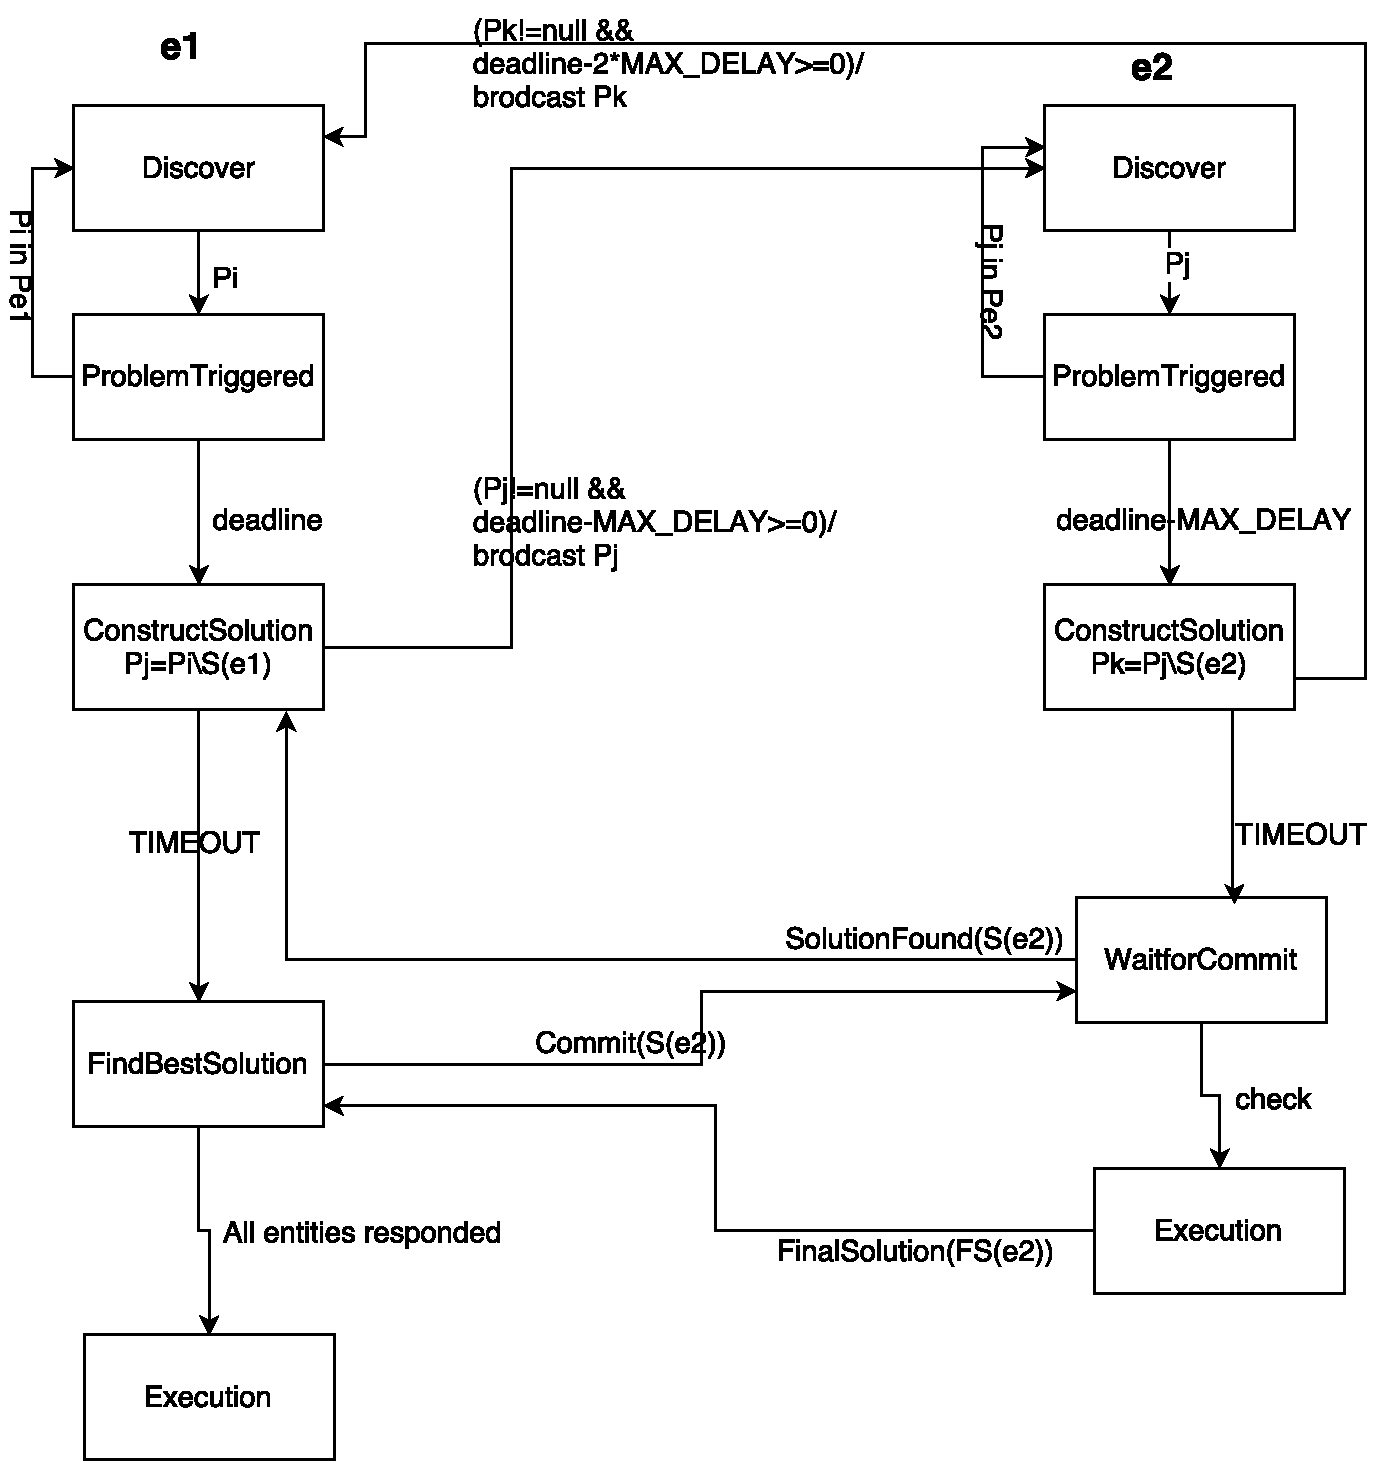
\includegraphics[width=3.25in]{Figures/MissionResolution_FK.pdf}
%\caption{Overview of the communication between two entities, problem triggered by the one in the left side}\label{fig:MissionR}
%\end{figure}


%<- robot_id; P <---- whole problem space
%S <---- global solution
%var timerV : machine;
%Target <----- target;
%sol <---- local solution$
%ri = myid();
%P={};
%S={};
%sol


%That being said, the only guarantees we can make about this resolution process is that the commited solution S(if everything goes well) will be executed.
%returns the current state of the global solution.
%The \textit{commit} event is a recursive function which goes through each participant in the resolution process and asks for resource commitment. Then, it updates the Behaviour Tree \textbf{(line 67)} with the current state of the local solution and it returns the current state of the global solution.

We can represent each instance of the resolution process as a tree, which we will call problem resolution tree (Figure~\ref{fig:MissionTree}). On top of the tree is an entity that triggered the general problem $P0$, while each node in the lower levels in the tree represents an entity that decompose the problem of its father entity and provides a partial/full solution. In the end, we have a resolution tree consisting of nodes representing the entities in one possible instance of the problem resolution process. We define a \textit{hierarchical order} in the resolution tree depending on the \textit{communication range} of the entities. The order of an entity in the tree  
is defined through the hop counter that refers to the number of intermediate entities through which an information must pass between the entity and the leader in the ensemble. For example in Figure~\ref{fig:MissionTree}, the leader e1 might not be able to communicate its problem P1 with the entities e5,..., e10 which are the leafs in the resolution tree because of the limitation in its communication range, but it might need few entities from the ensemble that are able to transit the information to the leafs (like entities e2, e3, e4) which are in the communication range of the leader e1, but also in the communication range of the leafs in the tree. The order of the entities that can directly communicate with the leader is higher comparing to the entities that need an intermediate entity to relay (in Figure~\ref{fig:MissionTree}, the leader e1 has the highest order, while the leafs e5,...e10 have the lowest order).

\begin{figure}[h]
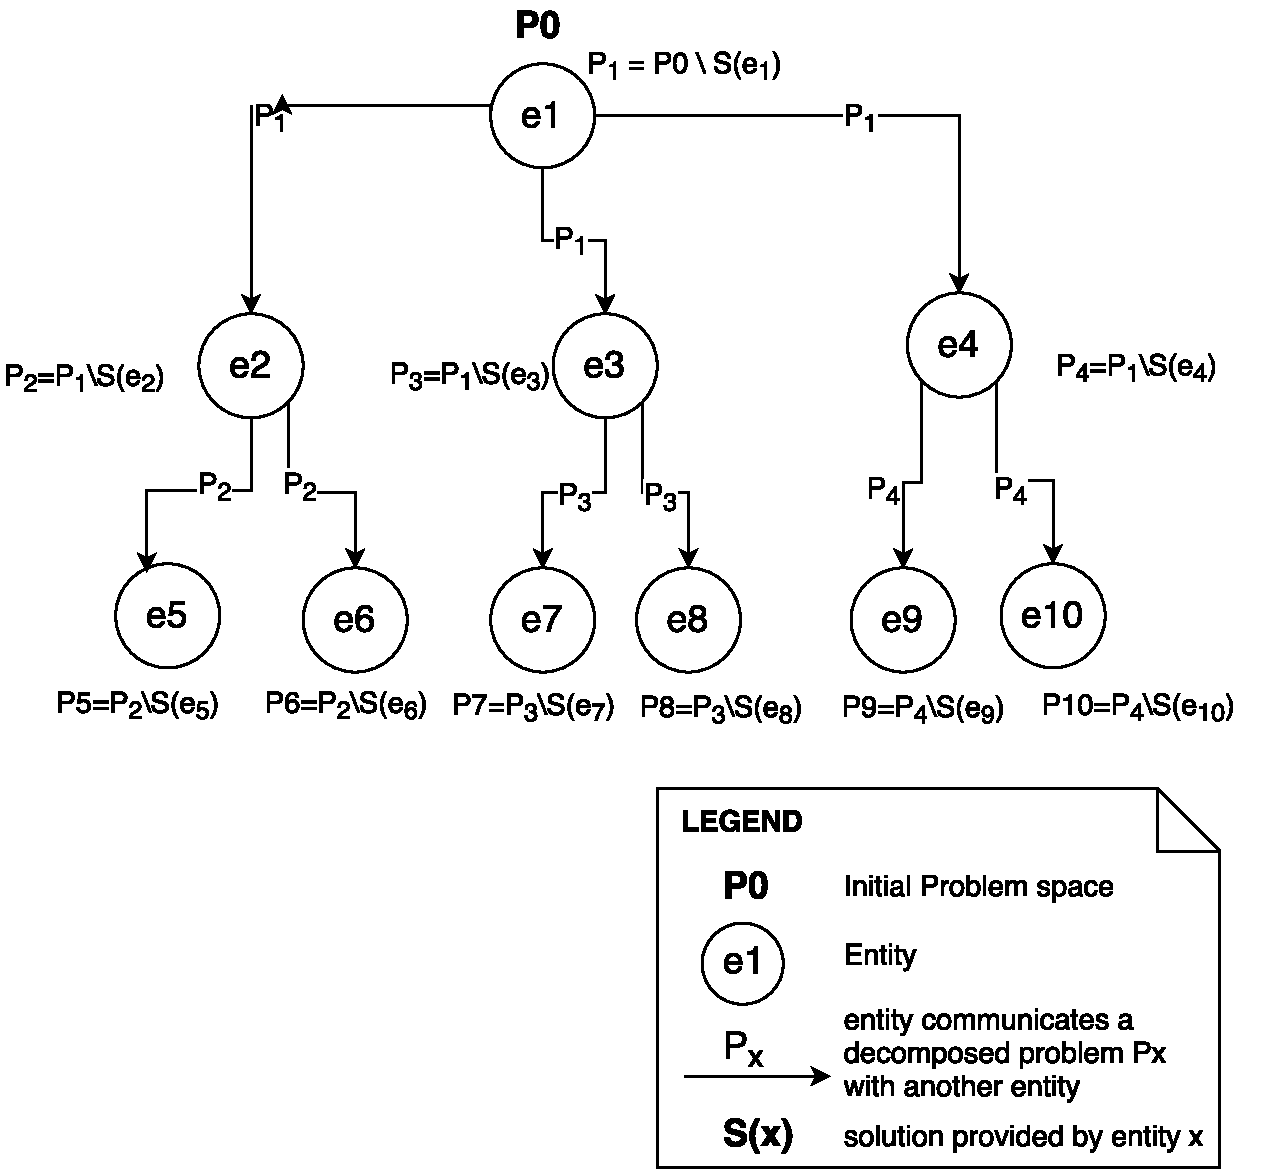
\includegraphics[width=3.25in]{Figures/ResolutionTree_FN.pdf}
\caption{Problem Resolution Tree}\label{fig:MissionTree}
\end{figure}

A formal definition of the problem resolution tree is as follows. 

\begin{definition}[Problem Resolution Tree]
A problem resolution tree is a tuple $T = (root, Ei, L) $ where:
\begin{itemize}
\item $root$ is the entity that triggered the top-level problem $P0$
\item $E_i$ are the nodes in the tree represented through the entities that decompose and partially solve part of the top-level problem
\item $L: N \mapsto N $are parent-child links between
entities that are able to communicate between each other. It is a function that represents problems/solutions communications from the root to its children.
\end{itemize}
\end{definition}

Each child in the tree decompose the problem received from its parent, so in the end we have a resolution tree where the leaves are entities that contain the smallest subset of the problem space. Each problem resolution tree represents only one possible instantiation of the problem resolution process. When the problem resolution tree have a full solution, the leafs' problem space  is an empty set.


%Finally, to understand how well the targets can handle the sub-problems, the function \textit{resolve} is called remotely on the targets (\textbf{line 22})
%and all possible solutions are memorized in S. The remote procedure waits for an answer from the targets until deadline d. 
%Once the solutions to sub-problems are obtained from
%the remote entities, the \textit{find\_best\_solution} is executed to identify the best solution \textit{sbest} and which combination of solutions contributes to \textit{sbest} (line 26). The function sbest is beyond the scope of this paper but generally is a domain and application specific.

%All solutions generated by the different solvers are stored in the list of possible solutions \textit{SolverList}.
%The best solution among all local ones is found using the function find\_best\_solver (\textbf{line 53-62}).

%The best solution is stored locally (function store). If
%the current entity is the resolution tree root (the first agent to invoke the function \textit{resolve}) (\textbf{line 33}), the function \textit{commit} is executed. 

%Function commit (\textbf{line 64-69}) enacts a distributed
%commit of the best solution. It takes as input the best solution
%and the set of involved agents in the specific problem resolution and 
%asks agent participants to commit their resources. 
%It should be noted that the time between the solution is proposed and the solution is chosen, some deviations of resources important for problem resolution might be encountered. 
%The \textit{commit} function is a recursive function which goes through each participant in the resolution process and asks for resource commitment. Then, it updates the Behaviour Tree \textbf{(line 67)} with the current state of the local solution and it returns the current state of the global solution.
%Our assumption is that there shouldn't be a big change in the solution quality between the moment a solution is proposed and a solution is chosen. That being said, the only guarantees we can make about this resolution process is that the commited solution (if everything goes well) will be executed.


%\patrizio{write as a theorem, theorem environment of Latex} 

\subsection{Correctness and completeness}
To resolve mission resolution problems we used a gossiping protocol that aims to disseminate the information about a specific problem and finds a solution. To prove the correctness and completeness of the approach, we need to prove correctness and completeness of the algorithm. 
Taking some additional assumptions, we prove correctness and completeness of the algorithm.
\subsubsection{Correctness} 

In order to prove that our algorithm is correct, we assume that the solvers provided by the different entities are correct. 
Correctness of a solver means that an entity's solver can generate a behaviour (solution) to resolve a particular mission related problem with a quality $q_a$. If that behaviour is executed correctly we have a correct adaptation.
We define a quality $q$ of a solution  $S_i$  based on two factors: (i) \textit{closeness} to the agent that triggered the problem, (ii) intrinsic quality given by the entity.
What we mean by closeness to the agent is the following: in one instance of the problem resolution tree, if there is an entity $e_k$ that has a \textit{higher order in the hierarchy} in the problem resolution tree 
%is \textit{hierarchically closer} 
%to the leader(entity that triggered the problem) 
and can propose a solution $s_k$ to a sub-problem $p_k$ , then we consider that the solution $s_k$ has precedence over solutions that are able to solve the same sub-problem $p_k$, but are coming from other agents that have lower order in the hierarchy in this instance of the problem resolution process.  
Because the communication between entities is limited, the algorithm is searching for solutions closer to the entity that triggered the problem $p_k$ and if it finds one, it stops the search for other solutions that are generated from entities that might produce solutions with better intrinsic quality, but are further from the leader. Thus, when we speak about hierarchy, we consider hierarchy of entities in terms of the problem resolution tree: the nodes that are closer to the root (meaning they need less number of hops to communicate with the root) have a higher order in the hierarchy comparing to nodes that are lower in the branching. Root has the highest order in the hierarchy, while the leafs have the lowest order in the resolution tree.
%hierarchy in the resolution tree.

The leader when calculating the best solution, doesn't have the exact information how each entity in the ensemble contributes towards the final solution. The only information the leader of the problem resolution process has when making the decision is how each entity that is directly reachable (it can directly communicates with) can help in resolving part of the the bigger problem of the leader. All reachable entities might have formed sub-ensembles that contribute towards the final solution, but the leader does not have that information.
For example a leader might be able to communicate with two entities that can provide some solution to the initial problem. Each of those two entities might have formed a temporary sub-ensemble. 
The two temporary sub-ensembles are on the same hierarchical level and they might have one entity in-common, however they belong to different instances of the resolution process and can be represented with two different problem resolution trees. When the leader decides for the final solution it might consider a combination of both sub-ensembles which create the final solution and chooses a final \textit{stable ensemble} that is a combination of both sub-ensembles. We can represent the stable ensemble in one instance of the problem resolution tree as in Figure~\ref{fig:MissionTree}.

The only guarantees we can make about this resolution process is that the committed solution (if everything goes well) will be executed. That being said, the assumption is that there should not be a noticeable difference in the solution quality between the moment a solution is proposed and a solution is chosen. Solution quality will remain the same if there isn't any change in the \textit{entity's resources} and in the \textit{connectivity formation} of the ensemble.
That is why we assume that the time between a solution is proposed and a solution is committed is really small so that there isn't any change in the \textit{connectivity formation} of the ensemble (\textbf{Assumption 1}).
%that  of the ensemble. Hence, we can say that the solution quality depends on these 
However, change in the resources for the proposed solution might come if an entity participate in two different resolution processes triggered by different leaders. During problem resolution, entities might propose solutions for different problems in different ensembles. As the resources of the entities are limited, we made the assumption that
%the quality of the commited solution is equal to the quality of the proposed solution meaning that
the entity will not participate in two different resolution processes (resolution processes triggered by two different leaders) which overlap in the usage of the resources i.e. 
if an entity participates in two different resolution processes from different leaders the usage of resources will not overlap (\textbf{Assumption 2}). 
However, there is another case that impacts the quality of the solution and that is when an entity tries to propose multiple solutions in one problem resolution process. Here, we will proof that with our algorithm that won't be possible. 
Thus, we define correctness as follows.

In these cases, we say that the committed solution quality is equal to the chosen solution quality. 
%Recollect that when computing a trajectory for a robotri
%, the execution
%of MRMP is decomposed into two phases: €rst the coordination
%protocol computes the avoid trajectories set Ψi which is then used
%by the safe plan-generator for computing the collision-free trajectory
%ξi



%Correctness of the algorithm is defined in terms of absence of deadlock in the commit function. That being said a deadlock might appear if there is a communication loop between agents in the ensemble. Hence, we provide the following theorem.

%\begin{theorem}[Correctness]
%For each instance of the resolution procedure for a problem $P_i$ we have a set of n \textit{different agents} that contribute towards the final solution $S_i$.
%\end{theorem}

\begin{theorem}[Correctness]
If an entity $e$ triggers a problem $P_i$ and Assumption 1 and Assumption 2 are true, then the Mission Problem Resolution Algorithm finds and computes the best quality solution $S_i$  proposed by an Ensemble $E$ that is in the communication range of the entity $e$.
\end{theorem}




\begin{proof}
As we mentioned earlier we assume that all mission related problems can be decomposed. Let's say we have an entity $e$ that triggered the problem $Pi$. $Pi$ can be decomposed on $m$ different different ways. For each different decomposition there is a sequence of local solutions proposed by an ensemble $E_m$  that combined together give a global solution $S_m$. The global solution $S_m$ is a sequence of local solutions $s_0, s_1, ..., s_k$, each of them with a particular quality $q_0, q_q, ..., q_k$ correspondingly. Let's assume there exists an ensemble consisting of \textit{n} entities for which there is a communication path between them and the leader (the ensemble might include the leader) and that they can provide the best final solution $S_i$ to a problem $P_i$. Correspondingly, we can decompose the solution to a sequence of local solutions $S_i=(s_0, s_1, s_2, ..., s_n)$ each with a particular quality  $q_0, q_q, ..., q_n$.  We can represent that ensemble using the problem resolution tree (Figure~\ref{fig:MissionTree}). 
In order to prove that the algorithm is correct, 
%we need computes the best quality solution 
we need to prove that the computed solution $S_i$ by the leader of the stable ensemble $E_n$ is the best for the problem $P_i$.
To prove that, we use the problem resolution tree of the \textit{stable ensemble}. The root of the tree is the leader. We need to prove that the solution calculated by the leader has the highest quality i.e. $S_i=(s_0, s_1, s_2, ..., s_n)$ each with a particular quality  $q_0, q_q, ..., q_n$.  
As our mission problem resolution is recursive at 
each node in the resolution tree, the algorithm calculates the best solution by considering the best combination of solutions proposed by its children. After calculating the best solution, it sends that solution to its parent. Starting from the leafs of the tree, the nodes calculate the best combination of solutions. In the end, the leader composes all combinations and calculates the best combination of solutions proposed by its children. If an entity proposed solutions to multiple problems in the same instance of the problem resolution tree, the algorithm will return a value which might not be correct because of lack of resources for the entities that proposed multiple solutions.
%Hence, we need to have a set of n \textit{different agents} in the \textit{stable ensemble} contributing towards the final solution $S_i$.

That is why we need to have (i) a set of n \textit{different agents} in the \textit{stable ensemble} contributing towards the final solution $S_i$  as a precondition for the leader to be able to correctly calculate the best possible solution. Our algorithm should not 
allow for one entity to participate with multiple different solutions in a same ensemble because as we mentioned earlier it might not be possible for one entity to perform multiple solutions due to a lack of resources.


To prove (i), we need to to prove that there is no possibility for a \textit{communication loop} in one instance of the problem resolution process (problem resolution tree).
What is considered as a possible loop in this distributed algorithm is a situation where one entity communicates a  sub-problem $P_j \in P_i$ with another entity that reduce the problem to $P_k \in P_i$ and communicates that problem to the first entity that triggered $P_i$. We can imagine a situation where before an entity commits its resources to a particular ensemble, it might propose solutions for other ensembles to resolve different problems, so in that case we might encounter a situation where the first entity will propose a solution to a sub-problem that was not able to resolve it before taking in consideration the whole nature of the problem (ex. in a previous iteration the entity proposed a solution to a more general problem and if it commits its resources to that solution, it might not be able to resolve the smaller problem that requires a solution in this iteration). To avoid that, each entity that runs the algorithm checks if the problem that is being received for resolution is some type of sub-problem of a more general problem that was being resolved in a previous iteration. If that is the case, the problem resolution procedure will not start i.e. the entity will not participate in the execution of the sub-problem.
%none of the logic in function resolve will be executed 
We verified (using model-checking) that this is always true. From here we can conclude that for each instance of the resolution procedure for a problem $P_i$ we have a set of n \textit{different agents} that contribute towards the solution $S_i$. In other words, there aren't two nodes in the tree that have reference towards same entity.




%To prove that we use contradiction. Let's assume there is a solution $L_i=(l_0, l_1, l_2, ..., l_m)$ that has a higher quality comparing to $S_i$. We can consider two cases: 
%(i)($S_i=L_i$) In this case, the solutions have same range (in our case that means the same area in the mission will be covered). However, the quality between them is different. We assumed that $L_i$ has a higher quality. From there, we can say that at least one portion of the solution $L_i$ has a higher quality (let's say there is some solution $l'_k=s'_m$ where $l'_k \in L_i \land s'_m \in S_i$ and where $qk, qm$  are their qualities correspondingly, we say $qk>qm$). 




% For each instance of the resolution procedure for a problem $P_i$ we have a set of n \textit{different agents} that contribute towards the final solution $S_i$.

Hence, we proved correctness of our algorithm.

\end{proof}


\textbf{Completeness}

Completeness of the approach is defined based on assumptions about the connectivity between the agents and the stability of resources and connectivity.
First, we assume that we have complete connectivity between agents meaning that starting from each agent we can broadcast a message that will reach all agents in the environment. 
Second, we assume that we have stable connectivity between agents which means that the connection between the agents will not disrupt during the adaptation process. 
Third, we assume that we have stable resources during adaptation which means that there isn’t a change in the resources important for the agent to execute the solution it proposes.
Taking in consideration these assumptions, we define the completeness of the approach as follows:
\begin{theorem}[Completeness]
If a solution $S_i$ for a specific problem $P_i$ exists and we have an infinite time (deadline $d$) to find it, the algorithm is able to find it.
\end{theorem}
\begin{proof}
If we represent one instance of the resolution process of problem $P_i$ as function that reduces problem $P_i$, then we can represent each reduction of $P_i$ in a monotonic decreasing sequence, each instance representing the appropriate reductions of the problem $P_i$.
According to the monotone convergence theorem [reference needed \darko{Where to find good reference for this}], if a sequence is decreasing and is bounded below by a minimum, in some infinite time will reach that minimum. In our case, the minimum would be the problem that corresponds to the final solution $S_i$ that in ideal situation will be the empty set.
Having that for all instances of the mission resolution process, we can conclude completeness.
\end{proof}


Proving that the algorithm will always find a solution, and that all participants in one instance of the problem resolution process are different, 



%In situations where the ROOT AGENT does not provide any type of solution, we have another agent that provides the full solution to the triggered top-level problem case. That is the ROOT LEADER ENSEMBLE. In situations where there is an overlap between the 

 %An Agent that has a SOLVER for a PROBLEM CASE. Sometimes this AGENT is same as the ROOT AGENT. That is in situations where the agent that triggered the PROBLEM CASE, contains a SOLVER that can solve the particular PROBLEM. However, if the AGENT that triggered the PROBLEM CASE does not contain a SOLVER, then the AGENT that provides a SOLVER for the PROBLEM CASE is called ROOT LEADER ENSEMBLE).
%If the AGENT is in the first category, it FORWARDS the information about the ACTIVE SOLVERS to its leader and waits for correspondence. If its SOLVER is chosen for activation, the LEADER sends request for reservation of resources. After the AGENT responds positively to the LEADER, he can transit to a state for EXECUTION. 







\section{Safety Problem Resolution} 

In this section, we discuss about the adaptation resolution problem related to safety problems. To be able to model specific safety related behaviours, we discuss few properties of agents and how they are connected to safety. %\patrizio{what will be in this section?}

%\section{Modeling Safety}

%Let $Coordinates = {(x,y,z) | x,y,z \in R}$  be the universal set of geographical coordinates where the mission takes place and let C be a point in that set.

%A region y is a subset of Coordinates in the three dimensional xyz-plane for which some condition $\Diamond $ is specified.



%\textbf{Region for reaction} is a three dimensional region of an agent that represents the minimum 

Here, what we mean by safety is the capability of avoiding undesired outcomes. In the MMMRs domain we consider actions that has catastrophic outcomes for safety and can't be undone by a finite sequence of other actions. 

We define what a \textit{safe MMRS} is. Informally, a MMRS is safe if:
\begin{itemize}
\item the configurations of all agents are safe. We denote with $conf(a_i, \tau)$ a boolean function that gives information if the configuration of the agent $a_i$ is safe at a particular time $\tau$.
\item the mutual interdependence of all robots configuration pairs involved during the whole mission is safe. We denote with $Dconf(a_i, a_j,\tau)$ a boolean function that represents the dependency of the configurations of agents $a_i$ and $a_j$ at time $\tau$. If it is \textit{safe}, the function returns true, otherwise if it is \textit{unsafe}, it returns false.
%The function can have two values \textit{safe} and \textit{unsafe}.
\end{itemize}

In the following we formally specify what a safe MMRS is. With MMRS we denote the set of all agents performing the mission (Definition 7) and with T the total mission execution time. 

\begin{definition}[Safety]
We say a MMRS system is \textbf{safe} at time $\tau \in T$ if and only if the following two points are valid:
\begin{itemize}
\item  $\forall a_i \in MMRS; conf(a_i, \tau)=true$.
 \item  $\forall a_i,a_j \in MMRS; Dconf(a_i, a_j,\tau)=true$.
\end{itemize}
\end{definition}

Before defining what types of configurations of an agent are safe (i.e. when $conf(a_i, \tau)=true$), and what type of interdependence of configurations of two robots is safe (i.e. $Dconf(a_i, a_j,\tau)=true$) we discuss few properties of agents.

We take a snapshot of the mission at a particular time $\tau \in T$. Now we define the following.
We denote with $OBS_\tau$ the region of all obstacles (known and uknown) in the environment at time $\tau$. We mentioned earlier that we define an Obstacle $o \in OBS_\tau$ as a region in the environment that should not intersect with the region of operation of an active robot(agent) to not jeopardize safety. 
%$ Obstacle = \{(x,y,z) | x \Diamond y \Diamond z \} $
We denote by $VR_\tau^i \in R $ the ``visible region" in which an agent $a_i$ can ``observe" its local environment (obstacles and other agent's location) at time $\tau$ and by $SR_\tau^i$ the \textbf{safety region} of an agent $a_i$  at time $\tau$ that represents a region that is the  absolute  minimum  separation  for  safety that must  be  maintained  during  a close  encounter  with  other (robots) agents  or with  a static/dynamic obstacle . 
In this work, we focus on one representation of safety defined through the concept of \textit{collision}. We define \textit{collision} as a situation when the safety zone of a robot is overlapping a region of an object or a safety zone of another robot at time $\tau$. In that context, we say that a MMR system is \textbf{safe}, if no collision happens during mission execution. Taking that in consideration, we define $conf(a_i, \tau)$ and $Dconf(a_i, a_j,\tau)$ in relation to collision avoidance. They are represented as safety invariants that must always be satisfied during mission execution  i.e. their value must always be \textit{true}.

%We want to explore all 


%Now we can define

%In the following, 

%and  safety in MMRSs systems with the following two safety invariant.\\
%Loc(i,t) is a geographical coordinate that represent the location of an agent Ai at time t. 

%We say that a MMRSs system is \textbf{safe}, if no collision happens during mission execution i.e. the following two safety invariants are always satisfied:

%Formally, we define them as follows:

\begin{definition}[Safety Invariants]
We define the following two safey invariants: $ \forall i,j \in MMRS  \quad and \quad \forall \tau \in T$ 
\begin{enumerate}
\item $ Dconf(a_i, \tau)=true \iff SR_\tau^i \cap SR_\tau^j  = \emptyset        $  
\item $  conf(a_i, \tau)=true  \iff  \forall o \in OBS_\tau;
SR_\tau^i \cap o = \emptyset $ \\
\end{enumerate}
\end{definition}



%\item $ \forall i,j \in A  \quad and \quad \forall \tau \in T;\\ SR_\tau^i(loc(i,t)) \cap safetyzone(loc(j,t)) = \emptyset        $      \\
% \forall i,j \in A  \quad and \quad \forall \tau \in T;\\


%\item $  conf(a_i, \tau)=safe  \iff  \forall i \in MMRS, \forall o \in Obstacle \quad and \quad \forall t \in T; \\
%safetyzone(a_i,\tau)) \cap o(t) = \emptyset $ \\


We defined SAFETY in Definition 21. with 1) and 2) as  absence of collisions. 
1) states that there will be no collision between agents, 
%while meaning their safetyzone will never intersect, 
while 2) states that there will be no collision between agents and obstacles during mission execution. 



%Our  framework  implements  aMission  Manager  componentas  part  of  the  Planning  component  in  the  MAPE-K  loopfor  each  entity.  The  mission  manager  receives  informationabout  the  eligible  mission  related  solvers  in  the  Knowledgecomponent. These are mission-specific and defined before thestart  of  the  mission.  Mission-specific  solvers  have  a  set  ofsolver  constraints  (configuration  parameters)  that  reduce  thespace  of  acceptable  problems  (ex.  a  solver  for  covering  ageographical  area  might  require  an  entity  to  have  an  activecamera,  enough  level  of  battery  etc.  to  be  able  to  resolve  aparticular problem).



Our framework implements a safety manager as part of the Planning component in the MAPE-K loop for each entity. The knowledge base of the MAPE-K loop contains a catalogue of correct obstacle avoidance algorithms as solvers which can be activated and able to provide a solution for an agent in a specific situation. These are solvers that can be reused in different application scenarios and missions independently of the type of the domain. Here,  the  scope  of safety specific  problems  is independent of the  nature  of  the definition of the mission.  

In  order to  explain  the safety  problem  resolution  process,  we  frame the  scope  of safety problems  for isolated  and  collective  adaptation. 
%An entity might perform isolated adaptation when facing with a  situation  where  its  behaviour  plan  trajectory  needs  to  passthrough  a  no-pass  zone.  In  this  case,  the  entity  might  have  asolver that generates a behaviour plan for avoiding a no-passzone. 
In our work, we envision resolution of the following types of safety problems: (i) collision with a static obstacle; (ii) collision with a  dynamic obstacle; (iii) collision between agents.  In the case of static/dynamic obstacle avoidance, an entity performs isolated adaptation i.e. one entity generates a solution(behaviour plan) to the problem. The  generated  solution  (behaviour  plan)  brings the entity  into  a  state  from  which  it  can  continue  executing the  mission. 
 Next,  we  will  speak  in  more  details  about  collective adaptation.

\subsection{Collective adaptation}

%For the third type of problems (collision between agents), the safety manager provides a palette of coordination protocols for the agents to be able to perform collision avoidance maneuvers. To resolve safety problems related to collision between agents, our framework uses the concept of ensembles. 

 %Further recursive calls are propagated using a remote procedure call for each participant in the safety ensemble. 



%In our framework we provide mechanisms which provides solutions to these type of solutions.


%For the first and second type of problems(Static/Dynamic obstacle collision), our framework provides a catalogue of correct obstacle avoidance algorithms as SOLVERS which can be activated and able to provide a solution for an agent in a specific situation. In the case of static/dynamic obstacle avoidance we have only one agent that provides a solution. 

For the third type of problems (collision avoidance between agents), our framework provides a palette of coordination protocols for the agents to be able to perform collision avoidance maneuvers. 
To resolve safety problems related to collision between agents, our framework uses the concept of ensembles described above.
Agents dynamically form collaborative groups using attribute-based communication ensembles as described in \todo{[reference needed]} to gain benefits that otherwise
would not be possible. In safety problem resolution, the agents must follow certain rules and in return the ensemble offers a guarantee that if all single agents follow the rules, safety will be preserved. Adherence to these collective
rules temporarily reduces the flexibility of the collaborating agents, but has a strongly positive impact on safety. Comparing to mission resolution where those collective rules are more flexible, the safety resolution requires stronger, more precise, and detailed rules. 


A safety ensemble is primary determined by the agents that collaborate to solve a safety solver. In a collision between multiple agents, our safety resolution procedure consists of: (i) a protocol for on-the-fly ensemble formation for safety resolution and (ii) a recursive function that is initially called locally by the ensemble leader to select and commit a solution. In the safety problem resolution, all entities in the ensemble must  participate in the solution creation because full solution is required. What we mean here is that we treat safety as binary (MMRS is safe or not). In contrast, in the mission resolution a partial solution is enough for solving a particular problem.
%Because of this perspective of the problem, all entities in the safety resolution problem must perform their corresponding behaviours for safety to be satisfied i.e. to have a full solution.
%Safety has a binary value (the system is safe or not), while  All participants in the safety ensemble must participate in the 
%because of its binary nature. What we mean by the binary nature is that  of the solution is that 
%s hard constraints, whose full satisfaction is required
%\ugh{because of the binary nature of the solution i.e. we might have full solution or not solution at all,
%which give a 
%full solution to the problem 
%while in the mission resolution a partial solution is enough for solving a particular problem}
%\patrizio{please explain better...not so clear}.
If one agent fails to comply to the rules in the ensemble, safety will be compromised. Here, the shape and structure of the ensemble is strongly correlated with the type of the safety problem due to the fact that all involved participants need to generate their corresponding behaviours to guarantee the safety of the system.


%If the safety problem is a type of collision between multiple agents,
%the resolution process consists of formation of an ensemble where all agents in the ensemble needs to participate in the solution creation. In contrast to the mission resolution where there isn't knowledge of which will be the agents that could participate in the resolution process, in safety resolution the knowledge of possible ensemble participants is known before the ensemble creation.
%In the end a full solution must be obtained for a safety problem in contrast to the mission problems where a partial solution is enough.




\begin{center}
\begin{figure}[!h]
 \lstinputlisting[language=sl, basicstyle=\scriptsize, tabsize=4,xleftmargin=3.0ex]{src/SafetyResolution.src}
%\lstinputlisting[multicols=2,language=sl, tabsize=2]{src/mainAnto.src}  
%\vspace{-0.2cm}
 \caption{EDL Specification for safety resolution ensembles} 
 \label {lstSafety}
 \vspace{-0.8cm}
\end{figure} 
\end{center} 
%(Leader.solution+Solver_Agent.solution)==FULL  
%(position,speed)
%(center, speed)     \forall a  \in VR(a1)
We  specify the ensemble  type  used  for  safety  problem resolution on Figure~\ref{lstSafety}. To identify the ensemble, we declare a leader  agent  to  be  the  id  of  the  ensemble - essentially saying that instances of this ensemble type cannot be created without the ensemble being associated with a unique entity instance, which can be seen as a coordinator of the ensemble. 
%\patrizio{please explain better. Moreover in the listing (row 2), is id a variable? Then what's Leader? As I understand Agent is the type} 
A Leader of an ensemble for safety resolution is an agent that leads the ensemble formation and decides for a safety resolution protocol.
%has knowledge of all ensemble members.
Example could be a fixed camera positioned in a particular point in the environment that checks if there is a possibility for collision between two or more robots or a robot that notices another robot in its visible region. Unlike the leader in the mission resolution ensemble, the leader in a safety resolution has knowledge of all the possible ensemble participants when decides for a solution type and when it starts the coordination of the problem resolution process.

%the process of coordination.
As we can see from Figure~\ref{lstSafety},
the  ensemble  membership  function  consists  of  three  sections as before. First, the structure of the ensemble is defined by declaring the ensemble roles the agents can play. In  our  case, same as in the mission resolution, an  agent  can  play one  of  the  following  roles in the safety resolution ensemble:
\begin{itemize}
\item Leader - an agent that has the highest safety index and leads the ensemble formation
%triggers the top-level PROBLEM\_CASE and leads the ensemble formation
\item Solver\_Agent  (an  agent  that  can provide partial solution that contributes towards the final solution)
\end{itemize}
Next,  we  place  semantic  constraints,  represented  by  the constraint  expression.  In  our  safety resolution ensemble a  constraint  for  an agent  to  be  part of  the  ensemble  is  that  there  must  be  a communication  link between  the  corresponding  agent  and its  leader.  What  we  mean  here  is  that the Leader can communicate with all ensemble participants. The other very important aspect in the ensemble formation is the solution space. In contrast to the mission resolution ensemble, a safety resolution ensemble must provide a full solution, so we put that as a constraint. Full solution consists of combination of behaviours generated by all participants in the ensemble. What we mean is that all ensemble participants agree to follow a specific protocol suggested by the Leader i.e. each entity in the ensemble must have a solver compatible to the solver proposed by the leader. Our assumption is that each entity has at least one solver that is compatible to the solvers of the rest of the system. We consider this assumption reasonable because we consider safety independently from the mission, so 
all safety solvers can be independently embedded in the knowledge base before the start of the mission independently of its type.  
%\patrizio{what's happen if an entity does not have a solver compatible to the solver proposed by the leader? Please explain here}. 
The third part of the membership definition  is  the  fitness  function, providing  information  about which  aspect  of  the  ensemble  membership  should  be  optimized. In  our  example,  the  fitness  function  is represented as maximized solution quality of the leader that coordinates all ensemble participants. 
Finally, knowledge exchange is specified, creating an information exchange between the members of the ensemble.  In  our  case,  we  have  exchange  of  three  types  of information.  First,  it is  the  information  of the agents' conflict region $conflict\_r$, which is calculated by the position of the agent and its corresponding speed 
%that generates the problem case
(line 13). The $conflict\_r$ is the safety region of an agent in a specific time interval during mission execution. Second, each of the entities in the  ensemble receives an information about a specific solver proposed by the Leader. Each entity in the ensemble receives information about a collision avoidance algorithm $A$ and the attributes of the algorithm $attr$ (example of attributes of the algorithm might be the central point around which the entities will perform the collision avoidance protocol,  their corresponding speed, etc.) (line 14).
Third, the leader gets information about the solution  of each entity in the ensemble (line 15).
%that  can  be  provided  by  each  agent  in  the  ensemble(line 14).


We defined the following protocol (Figure~\ref{fig:STMachine}) that is used for on-the-fly ensemble formation when agents discover that they are facing with a possible collision among them. Each agent starts executing in the \textit{Discover} state. 
If an agent $a_i$ notices other agents in its visible region, it broadcasts the $ReqforSafetyRegion$ event with identifier for the $VR$ - visible  region, the time $\tau$ when the message is sent and the identifier of the agent $id$, asking for the safety region $SR$ of the robots in its ``visible region" during some time period $\Delta\tau$. Then it goes to the \textit{WaitForResponse} state.

\begin{figure}[h]
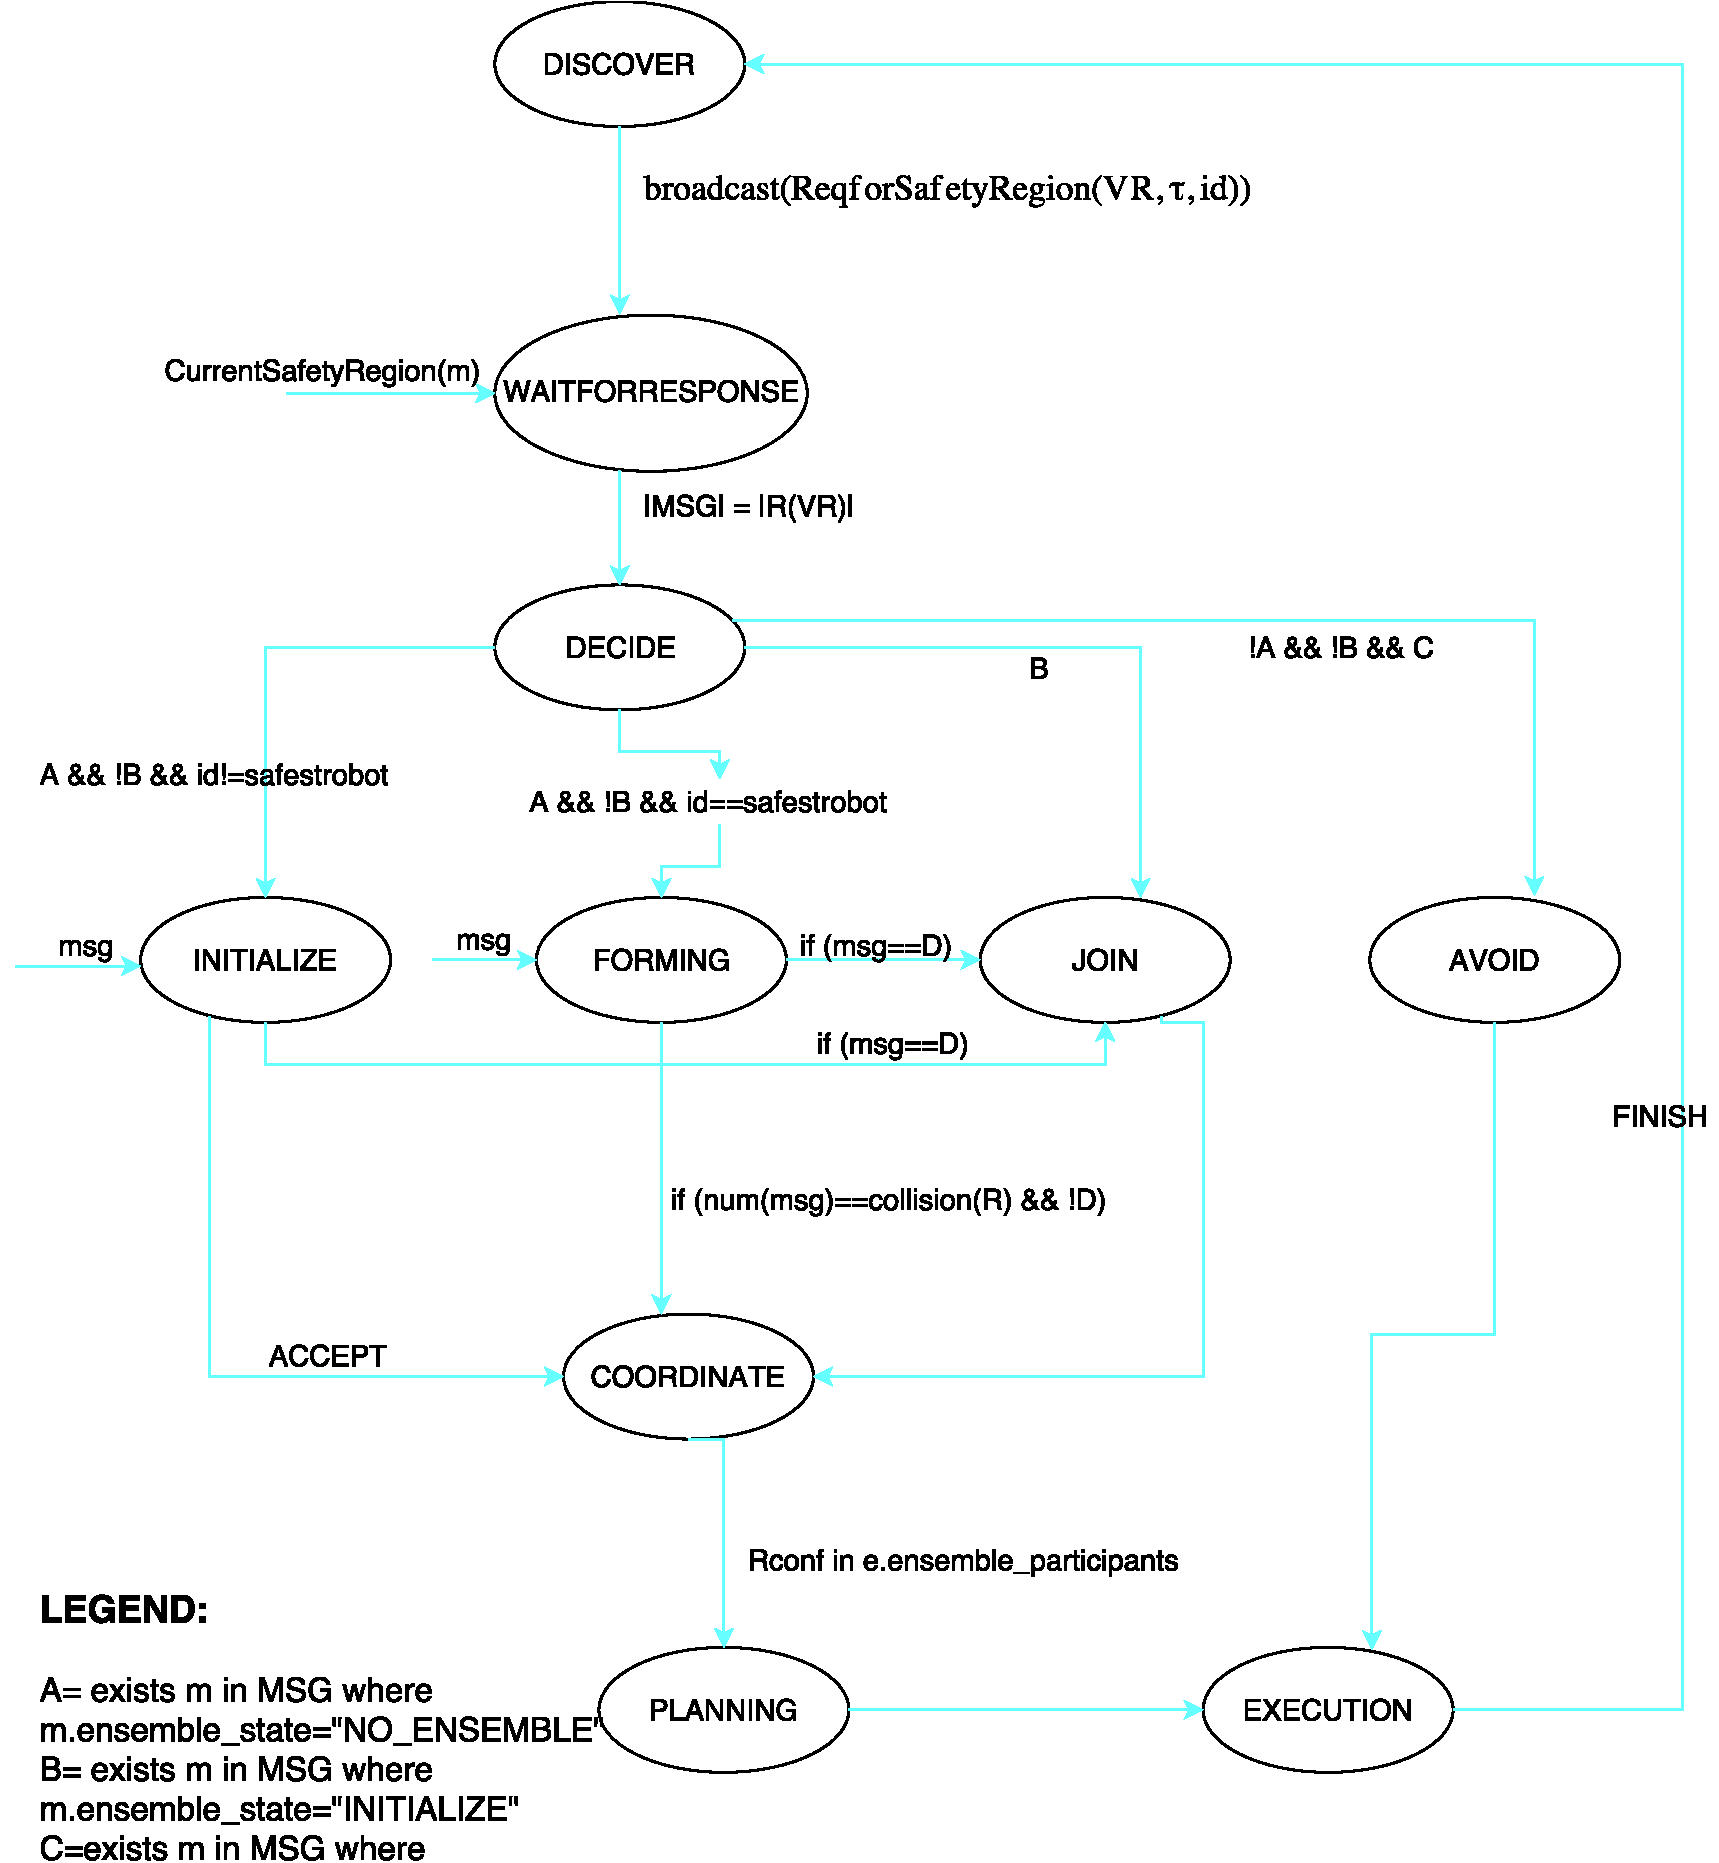
\includegraphics[width=3.25in]{Figures/SafetyResolution_FFFF.pdf}
\caption{State machine animating each entity in the safety resolution process}\label{fig:STMachine}
% \patrizio{better to represent states with circles instead of rectangles; it's more standard. Moreover the figure is unreadable}}
\end{figure}

%that consists of the following data
%checks if there could be a possible collision between the one that sends the message and itself. If the agent notices a possible collision, depending of its state
When an agent $a_i$ receives the event \textit{ReqforSafetyRegion(msg)}, depending of state it is, it generates a message  $m=(a_i:int;  conflict\_region:R; ensemble\_state:int)$, where \textit{$a_i$} is the identifier of the agent creating the message, the conflict region is a region in the environment that should not intersect with the region of operation of an active agent. If the agent is not part of an ensemble, the conflict region is equal to the agent's $SR^i_\Delta\tau$, while if the agent is part of an ensemble, it represents the \textit{execution region of the ensemble}, which is the union of the
$SR^i_\Delta\tau$ of all ensemble constituents. The ensemble\_state gives information if the agent is part of an ensemble and if it is, it gives information in which phase of operation the ensemble is. It can be in one of the following states: 
\begin{itemize}
\item \textbf{NO\_ENSEMBLE:} means that the agent is not part of an ensemble
\item \textbf{INITIALIZATION:}  means that the agent is a part of an ensemble that is in the phase of formation;
\item \textbf{PLANNING \& EXECUTION:}
means that the agent is a part of an ensemble that is established and it executes some safety-related algorithm that can't be interrupted at that time i.e. at the time of execution.
\end{itemize}


In the \textit{WaitforResponse} state, the agent $a_i$ waits to receive feedback from all the agents that were found in its visible region $VR$. When it receives message from all the agents in its visible region it goes to a state \textit{Decide}. In state \textit{Decide}, the agent goes through all messages and for each message it does the following: first, it checks if the agent $a_j$ that sends the message might collide with $a_i$.
%there is a possible collision between  \ugh{and itself}\patrizio{?}.  
If there is a possible collision it categorize the message in one of the following categories:
\begin{enumerate}
\item  \textbf{Category 1:} The message is from an agent $a_j$ that is a part of an ensemble in an initialization state (ensemble\_state=initialization). In this case, the agent $a_i$ considers the possibility to join to that ensemble, 
\item \textbf{Category 2:} The message is from an agent $a_j$ that is not part of an ensemble (ensemble\_state=no\_ensemble). Here, the agent $a_i$ considers the possibility to start with initialization of an ensemble.
%\patrizio{these items are difficult to follow. Use proper items}
\item \textbf{Category 3:} The message is from an agent $a_j$ that is a part of an ensemble that is in planning\&execution state (ensemble\_state=planning\&execution). In this case, the agent $a_i$ considers the conflict\_region received in the message as a dynamic obstacle and adds it in its collision region $CollisionR$. The ensemble in planning\&execution state can't be interrupted.
\end{enumerate}

After $a_i$ finishes the iteration through all the messages, it does the following decision:
\begin{itemize}
\item if there is at least one message from \textit{category 1} 
%an agent \ugh{that is in ensemble that is in an initialization phase}
(statement B in Figure~\ref{fig:STMachine}. is true), the agent $a_i$ goes to state \textit{JOIN} and initiates the joining process. 
%\ugh{In this state it considers all collision regions of the agents that are in an ensemble that is in execution phase as a dynamic obstacle and initiates the joining process.} 
If there are multiple messages from \textit{category 1}, the agent $a_i$ considers only joining to the ensemble which leader thas the highest safety index.  
%the highest identifier that is placed in the variable \textit{entity} (line x) agents that are in ensemble\_state==initialization.
\item %\ugh{If there isn't any message from an agent that is in ensemble that is in an initialization phase}
if there isn't any message from \textit{category 1} (statement B in Figure~\ref{fig:STMachine} is false), it checks if there is at least one message from \textit{category 2} i.e.
%an agent that is no part of any ensemble (ensemble\_state=``NO\_ENSEMBLE") i.e. 
if statement A in Figure~\ref{fig:STMachine} is true. If there are multiple messages of that kind, with the function \textit{findsafestrobot} it finds the identifier of the agent with the highest safety index in its visible region. If the agent has the highest safety index in its visible region, it goes into state \textit{FORMING} from where it starts the initialization of the ensemble, otherwise it goes into state \textit{INITIALIZE}.
\item This is the case when the agent has received only messages from agents that are parts of ensembles that are in their planning\&execution phase (\textit{category 3}). In this case the agent $a_i$ goes into the \textit{AVOID} state where the agent acts as it discovered a dynamic obstacle. In this state the agent should activate some of its solvers for dynamic obstacle avoidance that are able to generate a behavior(solution) for a dynamic obstacle avoidance. Here, the agent performs isolated adaptation and threats this problem on the same level as a dynamic obstacle.
%and threat the whole ensemble conflict region as a dynamic obstacle.
\end{itemize}

We define conflict set $Rconf$ for an entity $e$ as the set of entities that are in its visible region, can collide with $e$ and are not part of an ensemble that is in planning\&execution phase (entities that have send messages from category 2 and category 3). This means that $Rconf$ entities are ``open" for performing an appropriate collision avoidance protocol that should avoid the possible collision.

From the \textit{INITIALIZE} state, the entity waits for a message \textit{m} from the agent that has the highest safety index in its visible region to decide in which state it should go. If it receives a message  that there exists another entity with a higher safety index (statement D is true), it transits to a \textit{JOIN} state from where it starts the procedure for joining an existing ensemble. 
Otherwise, if it receives an \textit{ACCEPT} message means that the agent with the highest safety index in its visible region started the process for ensemble creation, and then it goes to a state \textit{Coordinate}. That means that there isn't any other entity with higher safety index in both of their visible regions.\\
The entity in the \textit{FORMING} state is a possible leader(coordinator) of an ensemble. The entity in this state sends ensemble ``proposal" requests to the entities that are in its vision region and have safety regions that overlaps with its safety region at some point of time in the future.
%announced a possible conflict meaning their safety regions at some point of time might overlap.
The entity  $e_i$ stays in the \textit{FORMING} state until one of the following happens: 
\begin{itemize}
\item  it receives a message from an entity in its visible region that ``rejects" its ensemble ``proposal" meaning that the entity that send the message ``knows" about another entity that has a higher safety index, so that entity should be the coordinator/leader of the ensemble (statement D is true). In that case, the entity that received the message directly goes into state \textit{JOIN}.
\item it receives a message from all entities in $Rconf$ and they all accepted the proposal for ensemble creation.
%its conflict zone \darko{define conflict zone earlier}
%visible region that might collide with it 
%\ugh{that they agree with the proposal for ensemble creation}. 
That means statement D is false i.e. there isn't any entity in $Rconf$ that "knows" about other entity $e_j$ that
%with higher safety index  \ugh{there isn't any entity in its visible region that knows about other entity that}
is in the \textit{FORMING} state and has a higher safety index.
\end{itemize}

%rejection from an agent that 
In the \textit{Coordinate} state, 
the coordination between the different entities in the ensemble happens.  The entity stays in this state, until all entities represented with Rconf are part of the ensemble. 
%Rconf represents an array of entities in the visible region of one entity that might collide with it and are not part of an ensemble that is in the state of planning\&execution.
When each of Rconf entities join the ensemble, the entity
goes into a \textit{Planning} state. The last entity that enters the \textit{Planning} state is the leader. When the leader enters this state,  on-the-fly ensemble formation phase finishes and the final ensemble is formed. 
Here, the leader has information for all ensemble participants and the final conflict region of the ensemble.
In this state the leader makes a decision of what is the best solver i.e.  what is the best collision avoidance protocol that all ensemble participants should follow. We implemented that by using the function $coordinate()$  %\todo{9}\patrizio{please use latex commands to refer to figures. Moreover, you probably wants to refr to Listing 4}, 
which is executed only by the ensemble leader (Figure~\ref{lstCodeSafety}). 
%\ugh{Based on the ensemble information it lists a prioritized list}
Based on the information about the ensemble (conflict regions, participants etc.), the leader generates a prioritized list of all possible solvers (list of collision avoidance algorithms) embedded in the Knowledge base that could solve the possible collision for this ensemble formation (line 3). 
Then, the ensemble leader starts from the first algorithm and calls the recursive function resolve\_safety(A, id, e\_j) where A is the algorithm that is chosen for safety resolution, id is the identifier of the entity that executes the algorithm to generate a solution and e\_j is the identifier of the entity that triggered the algorithm in the entity that executes it. 
Initially resolve\_safety(A, id, e\_j) is called locally by the ensemble leader so it has the form resolve\_safety(A, id, id) (line 5).

The function resolve\_safety includes the following.
%It lists all possible solvers embedded in the safety manager. First, function callSolvers finds all possible solvers that can solve this particular problem and prioritizes them (line 5). 
First, the appropriate solver is called to generate a solution S based on the algorithm A (line 10). 
%For each solution, starting from the top ranked, 
Then, a corresponding communication is derived using derive\_coms for each of the reachable entities in the ensemble. In other words, derive\_coms finds all the children in the problem resolution tree reachable from the corresponding entity in the final ensemble.
%in the safety resolution process.  
%If no other agents are involved in the solution, we associate the corresponding solution with the final one.

For each identified entity, the function resolve\_safety is called with the algorithm A (line (13)) 
and a solution $S$ is calculated. 
%A solution is calculated by remote invoking the resolve\_safety function
%and the solution is memorized in $S$.

The function resolve\_safety returns a boolean: 
\begin{itemize}
\item it returns true when the entity and all its children in the problem resolution tree contain the algorithm A in its knowledge base.  If that is the case, the generated solution $S$ is stored locally (function store (line 18));
\item it returns false when the entity itself or one of its children(targets) doesn't contain the algorithm A in its knowledge base.
\end{itemize}

In the end the resolve\_safety for the ensemble leader (line 5) returns true if all the entities in the ensemble are able and agreed to perform some algorithm $A$. If that is not the case, the ensemble leader goes through the other algorithms in the $SolverList$ and repeats the process until finds a suitable algorithm $A$ for which all ensemble participants are able to perform it. If it finds one, it calls locally the function \textit{commit} and breaks the loop. Execution of the commit function is when the entity enters the Execution state in Figure~\ref{fig:STMachine}.

%If other agents are involved in the safety problem resolution, 
%a set of solvers is identified across all reachable entities. A solution is calculated by remote invoking of the
%callsolvers function on the targets (line 14)
%and the solution is memorized in S.
%If a full solution is found (line 17) - meaning all agents involved in the problem provided a solution, the root agent that triggered the problem asks the participants to follow the protocol by using the commit function. \\ 
The \textit{commit} function 
{Line 23-26.} is recursive, it goes through each entity in the ensemble and enacts a distributed commit of the best solution. It updates the solution in each entity by updating its Behaviour Tree with the function update(S) (line 26).
When the entity finishes with the \textit{commit} function in the Execution state, it goes to \textit{Discover}.


%of the entity that 
%i calls the  goes from the beggining of the list and it calls the

%For each algorithm proposed by the ensemble leader
%a recursive function 

%After making that decision, it sends its decision to all ensemble participants the leader sends which

%and 
%In the planning state 
%i.e. it   that confirms  that acce












%To resolve safety problems, we abstractly define an algorithm that covers the procedure for safety problem resolution.
%The function is called locally by an agent that originally detected a Problem Case. In our case, the agent that detects this problem is placed centrally and has bigger global picture of the network.

%If more agents detect the problem, the agent will lowest id leads the resolution process.





\vspace{-0.3cm}
\begin{center}
\begin{figure}[bht]
 \lstinputlisting[language=sl, basicstyle=\scriptsize, tabsize=4,xleftmargin=3.0ex, ]{src/safecode.src}
%\lstinputlisting[multicols=2,language=sl, tabsize=2]{src/mainAnto.src}  
 \caption{Code snippets from Planning and Execution state} 
 \label {lstCodeSafety}
\end{figure} 
\end{center} 
 %\vspace{-0.8cm}



\patrizio{I am missing here a discussion about the correctness of the collective adaptation.}


\section{Related work}

In this section we review recent work on 
%modeling frameworks for multi-agent systems.
run-time modelling for mobile multi-robot systems. We investigate what kind of run-time modeling approaches are proposed for the different multi-robot systems and in which type of environments they are applicable. Furthermore, we focus at  identifying and  classifying approaches that address safety. Our aim is to understand how safety is managed and what are the constraints and limitations of existing methodologies  addressing safety.
Additionally, we consider if the approach supports adaptation on the system and which adaptation decisions  could be made at run-time.

 %\ivano{add table}\darko{I should classify all the related works from some of the previous papers and some part of the mapping study in one of the sections and create the table},
In Table, we note some of these run-time modeling approaches and categorize them according to the following criteria:
%\patrizio{why these criteria?}:
\begin{enumerate}
\item System \& environment characteristics;
\item Safety management;
\item Adaptation mechanisms
\end{enumerate}




For each criteria we identify several parameters.%\patrizio{explain better}
For each of them, we categorize the approaches as follows.
%\patrizio{why in this way, please explain}.



\renewcommand{\arraystretch}{1.0}
\begin{table*}[bth]
\footnotesize
\begin{tabular}{|c|c|c|c|c|c|c|c|c|c|c|c|c|}
\hline
\multirow{2}{*}{{\bf Work}}&
\multicolumn{6}{|c|}{\textbf{System \& environment characteristics}} 
&\multicolumn{2}{|c|}{\textbf{Safety Management}}
&\multicolumn{3}{|c|}{\textbf{Adaptation mechanisms}}\\
\cline{2-12}
& A. Type & Openness & Ens. type & Mgmt. & Hierarchy &  ENV & Coop. Mechanisms & Concerns sep. & Adapt &Type  & Human \\
\hline

\cite{cui2014refresh} & Heterogenous & N/A & dynamic & N/A & N/A & N/A & cooperative & NO & YES & BOTH & NO\\
\cite{parker1998alliance} & Heterogenous & YES & N/A & N/A & NO &  dynamic & local & NO & YES & isolated & NO \\
\cite{morais2015distributed}& Heterogenous & NO & N/A & N/A &  N/A & dynamic & cooperative & NO & NO & N/A & N/A  \\

\cite{khan2015framework} & Heterogenous & NO & dynamic & distributed & NO & static & cooperative & NO  & YES & isolated & NO\\
\cite{castello2016adaptive} & Homogeneous & NO & N/A & N/A & NO  & static & local & NO & YES & isolated & NO\\
\cite{desai2017drona} & Homogeneous & NO & N/A & N/A & NO & static & cooperative & NO & NO & N/A & NO \\
\cite{decastro2018collision} &  Heterogenous & NO & N/A & N/A &  NO & dynamic & centralized & NO & YES & N/A & N/A \\
\cite{desai2016dynamically}  & Homogeneous & NO & dynamic & centralized & NO & N/A & centralized & NO & NO & N/A & N/A\\
\cite{alrahman2016power} & Heterogeneous & YES & dynamic & distributed & YES & dynamic & N/A & N/A & YES & BOTH & NO \\
%\cite{bozhinoski2016leveraging} & Heterogeneous & YES & static & distributed & YES & dynamic & cooperative & YES & YES & BOTH & YES\\
\hline
\end{tabular}
\caption{Literature Comparison}
\label{tab:literature}
\end{table*}



\textbf{\textit{System \& environment characteristics}}

\begin{itemize}
\item \textbf{Agent type}: whether the considered agents in the system are homogeneous or heterogeneous. 

\item \textbf{Openness}: whether the approach supports systems that can accept external agents at run-time (e.g., new robots entering the mission). 
%\item \textbf{Context-awareness:} whether the framework supports systems that are able to understand key properties about its operational context (e.g., presence of obstacles, existence of other robots, etc.).

%\label{lbl:type} 


\item \textbf{Ensemble type}: whether the proposed approach supports formation of an ensemble(group of agents) and if yes, is the ensemble structure static or dynamic meaning is it possible for the ensemble structure to change at run-time. %For example, all the works focusing on a particular application scenario (e.g. supply-chain, grid market) will be considered as treating homogeneous agents.\\
	%\item \label{lbl:beha}
%\textbf{Agent Cooperation}: whether agents in the system act in a selfish or cooperative way.
	\item \label{lbl:confl}
\textbf{Ensemble management}: whether an ensemble is managed in a centralised or in a distributed way. %(ex. if there is a central entity that manages the ensemble)
	\item \label{lbl:hierarchy}
\textbf{Hierarchy}: whether the approach provides a mechanism for hierarchical structure of ensembles (e.g. an ensemble of ensembles).
\item \textbf{Environment} (dynamic vs. static): whether the approach supports modeling of systems that operate in environment that can change at run-time (e.g., moving obstacles, some other elements outside of the system can change their status) .
\end{itemize}
%The management here includes: the entrance of an agent in a coalition, the exit of an agent from a coalition, the adjustment of some parameter of the coalition itself etc.\\


\textbf{\textit{Safety Management}}

\begin{itemize}
\item \textbf{Cooperation mechanisms}: whether the approach allows safety mechanisms which involve cooperation between different agents rather than centralized management of safety entity or local management on
single robots, without any cooperation.

It is \textit{LOCAL} if safety mechanisms are conceived to work  on
single robots, without any cooperation,
 %Example of a centralized management (meaning there is an entity in the system managing the whole safety aspect).
\textit{CENTRALIZED} if the knowledge
of the overall system is maintained by a centralized entity,
or \textit{COOPERATIVE} if there are mechanisms to share knowledge between different robots that take part in the
mission.

\item \textbf{Separation of concerns}: whether the approach keeps the management of safety-specific issues (e.g. safety rules)  separated from the management of mission-specific issues
\end{itemize}

\textbf{\textit{Adaptation decisions}} 
\begin{itemize}
    

\item \textbf{Adaptability}: whether the approach supports MMRSs that can adapt
\item \textbf{Type}: whether the approach supports a collective adaptation where a collection of autonomous agents collaborate together to satisfy a particular goal or isolated adaptation where one agent adapts independently from the rest of the system
\item \textbf{Human Controllability}: whether the approach enables an operator (human) to be involved in the adaptation process. 
\end{itemize}


As shown in Table~\ref{tab:literature}, most of the approaches are unable to deal with open systems (only 2/9 approaches are able to deal with open systems).  By open systems, we mean systems that can accept external entities at run-time (e.g.,  new robots,  new human actors).   This implies that  most  of the  approaches  that  have  been  proposed do not consider that the system evolves in terms of addition or removal of robots and/or other types of agents, including humans.  This is indeed an interesting research direction since  systems of the near future will be necessarily characterized by openness, and it is often impossible to assess at design time the exact boundaries and topology of the system.

A  peculiar  system  characteristic  is  the  capability  of managing  teams  consisting  of  robots  of  different  types  (e.g.,robots for grabbing objects,  for video streaming,  sensing and discovering  relevant  information). According  to  Table~\ref{tab:literature} most of the analyzed systems have the capability of managing heterogeneous robots which is the direction in which we are going with our approach. 

In order to manage different unpredictable situations of missions and considering situations where there is only partial communication between different agents,  it is preferable  that  the MMR system is capable of grouping and regrouping agents in ensembles at run-time in a  decentralized fashion.  
Most of the approaches propose solutions where they assume that all robots in the system will be able to communicate to each other. Only 2/9 approaches discuss about the possible benefits of distributed ensemble formation. 
The concept of an ensemble enables single agents to take part in a group where they will follow certain rules and in return the ensemble offers certain advantages with respect to a preservation of a particular system quality. In this context, we don't need to consider the whole system to analyze if a particular system quality is satisfied, we only consider part of it.

Furthermore, as shown in Table~\ref{tab:literature}, in all approaches the management of safety-specific issues (e.g., safety rules) is not kept separated from the functional management of the robots (e.g., the mission). Keeping a separation of concerns means for instance that the approach prescribes a special layer for managing safety, which is totally separated from the rest of the system. 
%The only work where separation of safety-specific issues is considered is our previous work on which we build upon. 

Regarding the cooperation mechanisms,  most  of  the  approaches adopt  local  safety  mechanisms,  i.e.   safety  mechanisms  that are conceived to work on single robots, without any cooperation. Centralized safety management mechanism means that there exist an entity managing the safety aspect of the overall system. As can be seen in Table~\ref{tab:literature}
only 2 approach have a centralized safety management  mechanism.   Instead, 4  approaches  rely  on  co-operative safety mechanisms, meaning that safety mechanisms involve a cooperation between different robots.  

Regarding the adaptation mechanisms, most of the approaches allow the system to adapt at run-time, meaning that the system is able to adapt (e.g., behaviour adaptation, trajectory recalculation, goal renegotiation, etc.) in order to find a solution depending on some change in the context. Adaptability might be considered in conjunction with context awareness since awareness of the context is a required capability in order to support adaptability. Human involvement in the adaptation process brings some degree of control-ability that can help in defining regulations and rules about the responsibilities of the operators in operational scenarios and make adaptation more practical and safer. None of the approaches in Table~\ref{tab:literature} includes the human as a factor in the adaptation process.
Regarding the collectiveness of the adaptation process, 3 of the approaches consider isolated adaptation where the agent adapt its behaviour independently from the rest of the system, while only 2 approaches consider the two types of adaptation: (i) on a collective level where multiple agents must adapt altogether and transactionally
and (ii) isolated adaptation where one agent adapts its behaviour independently from the rest of the system. 


Classifying our framework in this classification schema is as follows:
It supports modeling of
  \textit{open systems} which consists of \textit{heterogeneous agents} that are \textit{context-aware} about their operational context. The agents can be grouped in \textit{dynamic ensembles} which are groups of agents that are managed in a \textit{distributed way} among the ensemble participants. Furthermore, the framework allows for a \textit{hierarchical structure of ensembles} for satisfying a particular goal as we showed in \cite{bozhinoski2016leveraging}.
Regarding the environment, the framework has mechanisms for modeling MMRSs that operate in \textit{dynamic environments} and have some degree of \textit{unpredictability} (ex. birds flying, animals walking etc).
%and can be used both in \textit{indoor} or \textit{outdoor} context.

Most of the frameworks we have analyzed do not consider safety aspects separate from the functional behaviour of the robots. In our framework we make a \textit{clear separation of concerns between safety and mission}. We consider this as extremely important for managing complex missions and it is one of the fundamental parts on which we base our framework. This way an operator modeling its mission can focus on the mission specification, while a safety engineer can focus on the safety-specific mechanisms, thus making safety-specific mechanisms reusable across missions, projects, and organizations.

Another really important feature of our framework is allowing \textit{cooperation mechanisms} between different agents when safety-related issues are triggered. This means that safety is not managed in a centralized way (there isn't an  entity that manages the whole aspect of safety, but it is managed on a level of ensemble in a distributed way where each agent should perform an appropriate behavior as part of the ensemble).


One of the decisions for designing the modeling framework is to be able system designers to design systems which are \textit{adaptable} during mission execution. Our framework allows part of the adaptation decisions to be done at \textit{run-time}. That being said, we make clear distinction about which decisions should be made at design-time versus decisions at run-time. Regarding the type, we allow agents to adapt on a collective(ensemble) level which means that a collection of autonomous agents collaborate to perform adaptation in order to satisfy a particular goal or solve a particular problem. 
In the end, we allowed the operator(human) be able to have control in the adaptation process. Some adaptation decisions can't be done by the system at run-time, however with our approach as we showed in \cite{bozhinoski2016leveraging} we allow the operator to take over and participate as agent in the adaptation process. 





\darko{END}

%\begin{lstlisting}[language=Python]
%function resolve_safety(pi,ai){
%sol=callSolvers(pi); 
%S=null; 
%if (sol!=0){ l
%	SolverList=prioritize(sol)
%	foreach (s in SolverList){
%			Target:= derive_coms(s)
%			if (Target is empty){
%				S=s;
%				
%			}
%			else{
%				foreach t \in Target
%					t.solution = rpc (callsolver(s, t))
%					S = S \union t.solution
%			}
%			if (|pi\{p(S)}|=null)
%				commit (S, Target)
%				break;
%		}
%	}
%}
%function commit(s, t){
%	store()
%}
%function commit(S, T){
%	foreach t in Target
%		t.update(S)
%	update(S)
%}
%\end{lstlisting}
The function includes the following important steps:\\
\textbf{Line 11-5}. It lists all possible solvers embedded in the safety manager. First, function callSolvers finds all possible solvers that can solve this particular problem and prioritizes them (line 5). 
For each solution, starting from the top ranked, a corresponding problem communication is derived using derive\_coms for each of the agents in the ensemble. If no other agents are involved in the solution, we associate the corresponding solution with the final one.
If other agents are involved in the safety problem resolution, 
a set of solvers is identified across all reachable entities. A solution is calculated by remote invoking of the
callsolvers function on the targets (line 14)
and the solution is memorized in S.
If a full solution is found (line 17) - meaning all agents involved in the problem provided a solution, the root agent that triggered the problem asks the participants to follow the protocol by using the commit function. \\ 
{Line 26-30.}The commit function goes through each agent in the safety resolution process and updates their Behaviour Tree in the Behaviour Manager component.



\darko{END}



The agent architecture consists of 4 components:
\begin{itemize}
    \item \textit{Behavior Manager:} containing information about the overall behavior of an agent. Here the behaviour plans are stored as behaviours in a Behaviour Tree. Each agent is assigned a Behaviour Tree. A behaviour tree is a run-time structure that represents the Behaviours associated with a specific agent. In the beginning of the mission, it contains all behaviours related to a specific agent $A_i$ to fulfill its part of the mission. During mission execution, the agent's behaviour tree may be updated as a result of violations in the behaviour plan with safety or mission related issues.
    %conditions.
   % Each behaviour in the Behaviour Tree is associated with a specific GOAL.
    \item \textit{Execution manager} is in charge of :(i) interacting with the \textit{Behaviour Manager} to receive the information about the status of the current behaviour, (ii) checking when safety-related conditions are violated in order to trigger the \textit{Safety Manager} which is safety-specific adaptation component, (iii) checking when mission-related conditions are violated in order to trigger the \textit{Mission Manager} to perform mission problem resolution and (iv) to log mission data.
    \item \textit{Safety Manager:} Contains "safety" solvers which are algorithms that generate a behavior for collision avoidance. These are agent-specific and defined before mission definition.
    \item \textit{Mission Manager:} Contains solvers which generate a behavior for completing parts of the mission. These are mission-specific and employed  before the start of the mission.  
\end{itemize}



\begin{figure}[h]
\includegraphics[width=3.25in]{Figures/CAdapt2.png}
\caption{Safety Problem Resolution\patrizio{unreadable}}
\end{figure}



%we envision the following: creation of dynamic ensemble are created using attribute-based communication grouping together agents that can see each other in specific regi.




In Figure 1, the Problem resolution for safety related issues is presented.

Here we will go for each of the cases independently and see how the state machine displayed in Figure 1 illustrates the process.

\subsection{PROBLEM Static/Dynamic obstacle}

In this case, we have an ensemble consisting of one AGENT\patrizio{please use the same notations used in previous sections. A generic agent can be $a_i$. The same for other entities.}. That AGENT is the ROOT(ENSEMBLE leader). 
In the initial state, each of the agents is monitoring its state and the environment where it is operating. When an AGENT performing a behaviour, notices that its AGENT CONTEXT MODEL is not aligned with its BEHAVIOUR CONTEXT a PROBLEM CASE (OBSTACLE) is generated and triggered. It checks if its KNOWLEDGE MODEL contains a SOLVER(Obstacle avoidance algorithm) that can provide a solution (a PATH) for this particular PROBLEM CASE. If it does not find a SOLVER, it goes to the state SOLVER\_NOT\_FOUND. In our framework, our aim is that an agent will never come to this state when a resolution for a safety issue happens. In order to ensure this never happens, we are providing an algorithm that is a DEFAULT SOLVER for safety problems. This SOLVER will always be able to calculate a PATH for an agent from its current location to its HOME.

When one or multiple SOLVERS are found, it transits to the state SOLVERS FOUND, from which it passes to the state SOLVERS INITIALIZATION. Here, the agent goes through the SOLVERS until finds one that can be executed. SOLVERS are prioritized according to system designer preference.

For each SOLVER that is found, the AGENT decides if the solver can be activated or not. If according the initial conditions(LOCAL DEMANDS GUARANTEED), the ALGORITHM can provide a PATH, the SOLVER goes into ACTIVE STATE. For this type of problem, we don’t need the collaboration of other agents, so we don’t follow that branch in the state machine. In the ACTIVE state, the SOLVER generates a new Behaviour according to the PROBLEM parameters. Then, the AGENT goes into state EXECUTE. Here, a new Behaviour is generated and its execution is started.
We call this a LOCAL ADAPTATION. 

%Here, we have shown LOCAL ADAPTATION.


\subsection{Collision avoidance among agents}

In this case, we have an ensemble consisting of multiple agents. In safety related problems, all members of the ensemble participate in the resolution process because we want to be able to guarantee safety for each member in the team. We distinguish between the following type of AGENTS in the ensemble:
\begin{itemize}
    \item ENSEMBLE LEADER (the agent that triggers the PROBLEM CASE)
    \item SOLVER PARTICIPANT (Agent which was contacted to help in the resolution process with its SOLVER)
\end{itemize}

In the initial state, each of the agents in the ensemble is monitoring its state and the environment where it is operating. Some or ALL of the AGENTS in the ensemble might notice a COLLISION between agents. All the AGENTS that notice a COLLISION, triggers a PROBLEM CASE. A Consensus about ENSEMBLE LEADER is done. In our work, we will consider the agent with the  smallest id as an ensemble leader. The ENSEMBLE LEADER continue the process by checking if its KNOWLEDGE MODEL contains a SOLVER (a coordination protocol, dynamic obstacle avoidance algorithm etc.) that can provide collision avoidance maneuvers.
If it does not find a SOLVER, it goes to the state SOLVER\_NOT\_FOUND. However, as we stated before there is always a DEFAULT SOLVER for safety problems to avoid this state.

If the ENSEMBLE LEADER finds one or multiple SOLVERS that can solve COLLISION AVOIDANCE, it transits to the state SOLVERS FOUND, from which it passes to the state SOLVERS INITIALIZATION. Here, the leader goes through each of the SOLVERS until finds one that can be executed.
How the check process works?
First, the AGENT checks if the initial conditions of the protocol defined in the SOLVER are satisfied. If that is not the case, it transits to INACTIVE state immediately and continue with the checking of the next SOLVER. If the initial conditions are satisfied, the ENSEMBLE LEADER sends REQUEST to the corresponding ACTIVE SOLVERS for each of the AGENT’s in the ensemble.
If there is a TIMEOUT (the Leader waited long enough and did not received an answer from all other AGENTS in the ensemble), the SOLVER becomes INACTIVE. It the AGENT receives information about other ACTIVE SOLVERS it transit to state: RECEIVED ACTIVE SOLVERS FROM ENSEMBLE PARTICIPANTS,  meaning the initial conditions of all ensemble members guarantee correct collision avoidance. The Ensemble Leader asks all ensemble members to commit to this ensemble and waits for confirmation. When a confirmation about commitment is received from all participants, the LEADER sends confirmation back and the ENSEMBLE enters in a critical section meaning the agents must stay in the ensemble and follow the protocol and the rules defined in it in order to not provoke a collision. In this point, the SOLVER is ACTIVE (a behaviour is generated) and the ENSEMBLE LEADER starts with execution by going into state EXECUTE.

For the ENSEMBLE PARTICIPANTS the following happens. They receive a request for a SOLVER. If the SOLVER is found, is initialized. In collision avoidance, SOLVER PARTICIPANTS do not provide SOLVERS that involve other AGENTS i.e. they have a local solution. From there, it is easy to check for them if they fulfill the initial conditions in order to become ACTIVE/INACTIVE. If they have an ACTIVE SOLVER, they communicate with the ENSEMBLE LEADER and confirm their commitment in the execution process. After confirmation about the commitment is received, the process of execution can start. 










\section{State of the Art}

In this section we review recent work on 
%modeling frameworks for multi-agent systems.
run-time modelling for mobile multi-robot systems.

In Table \ivano{add table}\darko{I should classify all the related works from some of the previous papers and some part of the mapping study in one of the sections and create the table}, we note some of these and categorize them according to the following criteria\patrizio{why these criteria?}:
\begin{enumerate}
\item System characteristics;
\item Environment characteristics;
\item Safety management;
\item Adaptation decisions
\end{enumerate}
For each type we identify several parameters.\patrizio{explain better} For each parameter we categorize the frameworks as follows\patrizio{why in this way, please explain}.



\renewcommand{\arraystretch}{1.0}
\begin{table*}[bth]
\footnotesize
\begin{tabular}{|c|c|c|c|c|c|c|c|c|c|c|c|c|}
\hline
\multirow{2}{*}{{\bf Work}}&
\multicolumn{6}{|c|}{\textbf{System \& environment characteristics}} 
&\multicolumn{2}{|c|}{\textbf{Safety Management}}
&\multicolumn{3}{|c|}{\textbf{Adaptation mechanisms}}\\
\cline{2-12}
& A. Type & Openness & Ens. type & Mgmt. & Hierarchy &  ENV & Coop. Mechanisms & Concerns sep. & Adaptability &Type  & Human \\
\hline

\cite{YeZS13} & \checkmark& & &\checkmark &\checkmark & &\checkmark & & &\checkmark & &\\
\cite{MihailescuVO11} &\checkmark & & & \checkmark&  \checkmark& & \checkmark& & &\checkmark & & \checkmark \\
\cite{Pinto}&\checkmark & & & \checkmark&  \checkmark& & \checkmark& & &\checkmark & \checkmark  & \\
\cite{SimsGL03}& \checkmark& & & \checkmark&  & &\checkmark & & &\checkmark &  & \checkmark  \\
\cite{RoohiS11}& &\checkmark & &\checkmark &\checkmark  & & &\checkmark & &\checkmark & & \checkmark \\
\cite{CoppoDV14}& &\checkmark & & &\checkmark  &\checkmark & &\checkmark & & & & \checkmark \\
\cite{PredaGGLM15}& &\checkmark & & &\checkmark  &\checkmark & &\checkmark & & & \checkmark & \\
\cite{NicolaLPT14}& &\checkmark & &\checkmark &  & \checkmark & \checkmark&  &\checkmark & & \checkmark &\\
\cite{HennickerK14}& &\checkmark & &\checkmark &  & & &  &\checkmark & & \checkmark &\\
\cite{niemczyk2015adaptive}& &\checkmark & &\checkmark &  & &  & \checkmark  && \checkmark & & \checkmark \\
\cite{zhong2011runtime}& &\checkmark & &\checkmark & \checkmark &  & \checkmark &   &\checkmark &  & & \checkmark \\
\cite{Yu2010} & & \checkmark & & \checkmark  & & \checkmark & \checkmark & & & \checkmark & & \\
\cite{Yu09} & & \checkmark & & \checkmark & & \checkmark
& & \checkmark & & \checkmark & & \\
\cite{WeynsMACODO10} & & \checkmark & & \checkmark & & \checkmark & & \checkmark & \checkmark & & & \\
\cite{Oliveira6676505} & \checkmark & & & \checkmark & & \checkmark & \checkmark & & & \checkmark & & \\
\cite{grassi2013qos} & \checkmark & & & \checkmark & & \checkmark & \checkmark & & & \checkmark & & \checkmark \\
\cite{Edwards2009} & \checkmark & & & \checkmark & & \checkmark  & & & \checkmark &  & \checkmark & \\
\cite{Sykes2011} & & \checkmark & & \checkmark & & \checkmark & \checkmark & & & \checkmark & \checkmark & \\


\hline
\end{tabular}
\caption{Literature Comparison}
\label{tab:dliterature}
\end{table*}



\textbf{\textit{System characteristics}}

\begin{itemize}
\item \textbf{Openness}: whether the framework supports systems that can accept external agents at run-time (e.g., new robots entering the mission). 
\item \textbf{Context-awareness:} whether the framework supports systems that are able to understand key properties about its operational context (e.g., presence of obstacles, existence of other robots, etc.).
	\item
%\label{lbl:type} 

\textbf{Agent type}: whether the considered agents in the system are homogeneous or heterogeneous. 

\item \textbf{Ensemble type}: whether the proposed structure of an agent ensemble is static or can change at run-time(dynamic). %For example, all the works focusing on a particular application scenario (e.g. supply-chain, grid market) will be considered as treating homogeneous agents.\\
	\item \label{lbl:beha}
\textbf{Agent Cooperation}: whether agents in the system act in a selfish or cooperative way.
	\item \label{lbl:confl}
\textbf{Ensemble management}: whether an ensemble is managed in a centralised or in distributed way.
	\item \label{lbl:hierarchy}
\textbf{Hierarchy}: whether the framework provides a mechanism for hierarchical structure of ensembles (e.g. an ensemble of ensembles).
\end{itemize}
%The management here includes: the entrance of an agent in a coalition, the exit of an agent from a coalition, the adjustment of some parameter of the coalition itself etc.\\

\textbf{\textit{Environment characteristics}}
\begin{itemize}
\item \textbf{Dynamics}: whether the framework supports modeling of systems that operate in environment that can change at run-time (e.g., moving obstacles, some other elements outside of the system can change their status) (DYNAMIC vs. STATIC).
\item \textbf{Predictability}: whether the framework supports systems where the dynamic environment is fully predictable at design-time (e.g., external entities can move but only in specific ways or trajectories etc.) or we can allow some type of unpredictability
\item \textbf{Context type}: whether the framework supports only modeling of context-dependent systems (Indoor/Outdoor environment vs BOTH).
\end{itemize}

\textbf{\textit{Safety Management}}

\begin{itemize}
\item \textbf{Cooperation mechanisms}: whether the framework allows safety mechanisms which involve cooperation between different agents rather the centralized management (meaning there is an entity in the system managing the whole safety aspect).
\item \textbf{Separation of concerns}: whether the framework keeps the management of safety-specific issues (e.g. safety rules)  separated from the management of mission-specific issues
\end{itemize}

\textbf{\textit{Adaptation decisions}} 
\begin{itemize}
    

\item \textbf{Adaptability}: whether the modeling framework supports system that can adapt
\item 
\textbf{Adaptation Type}: if the framework can model adaptable system, does it support decision making at run-time. 
	\item 
\textbf{Utility}: whether the adaptation decisions from agents depend on some notion of utility (meaning whether the decision making mechanism of an agent is based on some sort of metrics) and the agent use these metrics to produce plan for execution. 
\item \textbf{Collectiveness}: whether the framework supports a collection of autonomous agents to collaborate to perform adaptation to satisfy a particular goal
\item \textbf{Correctness and Completeness}: whether the framework provides mechanisms for correctness and completeness in the adaptation process.
\item \textbf{Human Controllability}: whether the framework enables an operator (human) to be involved in the adaptation process. 
\end{itemize}



Classifying our framework in this classification schema is as follows:
supports modeling of \textit{open systems} which are \textit{context-aware} about their operational context. It supports modeling of \textit{heterogeneous agents} which can be grouped in \textit{dynamic ensembles}. The behaviour of the agents is always \textit{cooperative} as we focus only on civilian missions and we consider safety as a first class element in the design of these systems. The ensemble is managed in a \textit{distributed way} among the ensemble participants.The framework allows for a \textit{hierarchical structure of ensembles} for satisfying a particular goal.

Regarding the environment, MMRSs operate in \textit{dynamic environments} which have some degree of \textit{unpredictability} (ex. birds flying, animals walking etc) and can be used both in \textit{indoor} or \textit{outdoor} context.

Most of the framework we have analyzed do not consider safety aspects separate from the functional behaviour of the robots. In our framework we make a \textit{clear separation of concerns between safety and mission}. We consider this as extremely important for managing complex missions. It is one of the fundamental parts on which we base our framework. This way an operator modeling its mission can focus on the mission specification, while a safety engineer can focus on the safety-specific mechanisms, thus making safety-specific mechanisms reusable across missions, projects, and organizations.

Another really important feature of our framework is allowing \textit{cooperation mechanisms} between different agents when safety-related issues are triggered. This means that safety is not managed in a centralized way (there isn't an  entity that manages the whole aspect of safety, but the safety is managed on a level of ensemble in a distributed way).

One of the decisions for designing the modeling framework is to be able system designers to design systems which are \textit{adaptable} during mission execution. Our framework allows part of the adaptation decisions to be done at \textit{run-time}. That being said, we make clear distinction about which decisions should be made at design-time versus decisions at run-time. Regarding the collectiveness, we allow agents to adapt on ensemble level which means that a collection of autonomous agents collaborate to perform adaptation in order to satisfy a particular goal or solve a particular problem. 
In the end, we proved \textit{correctness and completeness of the adaptation algorithms} employed in the framework.


%, on multi-party sessions and choreographies, on component ensembles and on run-time modelling for mobile multi-robot systems. 

%There are some works on formal modeling that leads the adaptation on architecture level. FORMS - FOrmal Reference Model for Self-adaptation  [1] is a reference model that consists of a small number of formally specified modeling primitives that correspond to the key variation points within self-adaptive software systems, and a set of relationships that guide their composition. It is in compliance with the MAPE-K loop. The difference with our work is that we formally specify the adaptation behavior of the entities in MMRSs. 
%In [2] is presented an approach that addresses collective adaptation of generic agents. We have identified the following limitations of that approach:
%•	There is no clear evidence that the approach is correct and complete. 
%By correct we mean that there is no evidence that the solvers that are found are solution to the particular problem.  By complete we mean that there is no evidence that if there is a solver that is a solution to a particular problem, the approach is able to find it.
%•	The approach does not provide any type of optimization in the selection procedure in terms of what is the best solver for a particular problem. (The approach does not provide any classification framework that defines which solvers are better for a particular problem and how the approach is able to understand that?)(which parameters and metrics should be used) 
%•	The approach assumes that only one issue can be raised in one moment. Multiple issues cannot be raised concurrently.
%•	The behavior of human is modeled as generic agent. There is no distinction between the different entities in the system (behavior of a robot and an operator). Separating the human behavior from the other entities of the system can help us to better understand the impacts of human involvement in the adaptation process (understanding the human controllability in the adaption process – how much the operator is involved in the adaptation) and can help in defining regulations and rules about the responsibilities of the operators in operational scenarios.

%For the design of MMRSs systems





%It includes the following steps:
%Lines 19-20. Execute is called for each of the target entities
%corresponding to the best solution. Execute is an asynchronous
%function, so as not to impede the solution execution on line
%21.
%Line 21. Entity e executes the internal solution corresponding
%to the best solution.











%Each Problem Case includes a set of parameters describing it. 

%The PROBLEM CASE is always produced by the agent that has SET OF PROPERTIES that violate its behaviour context. 




%Solver is a function that as input algorithm that can be activated by an AGENT to produce a behaviour that will align the Agent context model to the corresponding Behavioural context  i.e. will produce a behaviour that is a solution to an appropriate PROBLEM CASE.



 
% We define a measure of satisfiability that uses the problem hbased
%distance to an accepting state in the DFA Acosafe. L
 

%(all tasks are in state COMPLETED (Figure x)).


%We study the meaning of partial satisfaction of 
%liveness requirements. T
%number 

%Here, we present a method for proving partial satisfaction for the liveness (soft) constraints to
%appropriately attend to the user’s (unexpressed) intentions in
%different types of specifications (e.g., sequential and temporary
%conditions on goal visits in addition to coverage) while still satisfying
%the safety (hard) constraints


\newpage
\clearpage

\section{Introductions}
 Mobile Multi-Robot Systems (MMRSs) are an emerging class of systems that adapt their behavior at run-time to achieve specific goals. They are represented by a set of mobile robots operating as a team with other agents (even together with humans) in a shared environment. In the literature, a variety of definitions exists defining the term robot [4–6]\patrizio{put proper references}. All of them share the following concept: a robot is an intelligent device with a certain degree of autonomy that contains sensors, control systems, manipulators, power supplies and software all working together to perform the required tasks. Under this perspective, a mobile robot represents a robotic system consisting of a SW/HW platform carried around by locomotive elements and able to perform tasks in different contexts. The kind of locomotion that the robot is able to perform is primarily decided upon the environment (aquatic, aerial or terrestrial) in which the robot will be operating [7].\patrizio{put proper reference}  Mobility gives robots enhanced operative capabilities, but at the same time increases complexity and brings additional challenges.
 
 
\textbf{PROBLEM STATEMENTs}

 MMRSs should be able to operate under highly dynamic conditions. \patrizio{do you refer to dynamic conditions of the environment? Probably is better to mention not only dynamism but also uncertainty and uncontrollability. These are different facets that give a measure of the complexity.}
%\ivano{add a couple of examples}). 
Highly dynamic conditions introduce a set of uncertainties\patrizio{dynamism does not necessarily implies uncertainty. Explain better} resulting from incomplete knowledge of the run-time structure of the system \patrizio{what do you mean by runtime structure of the system?} and the environment at design time\patrizio{explain better also that}. Incomplete knowledge of the run-time structure of the system comes from its openness. By ``open" we mean that new entities can join or leave the system at run-time. Incomplete knowledge of the environment comes from its dynamics (e.g., a bird flying in the environment). The consideration of the environment when specifying the system comes due to the fact that a mission is always associated with a physical context where it is happening, so how a system will perform a mission strongly depends on the environment where it operates (e.g., the system will operate differently in environments with smooth vs. rough surface, environments  with a lot of static obstacles vs environments with a small number of obstacles etc). 
%We consider the environment at design-time we define mission because (usually) a house does not move at runtime, so the planning of the trajectories can benefit from knowing this info beforehand) as to define a mission we always locate it in a specific  in our de part of the )\ivano{explain why the knowledge is incomplete at run-time, and why it will always be like that, that is: there is some information that is not known at design time by definition (e.g., a bird flying into a drone)} and the environment at design time \ivano{what do you mean by environment here? The physical environment? If it is like that, then you have to explain why you consider the environment also at design time since many approaches do not make any assumptions on it at design time. We do it because (usually) a house does not move at runtime, so the planning of the trajectories can benefit from knowing this info beforehand)}.
Handling uncertainty upfront is often infeasible (or expensive). This means we need to deal with it when the knowledge becomes available and perform system adaptation. 
To perform adaptation, the system needs to decide how to adapt. There might be few ways adaptation to happen \ivano{this sentence seems incomplete}. That \ivano{that whay?} requires identification of variability points of the system at design-time \ivano{this is already part of the solution.}. Variability among MMRSs is multi-dimensional since changes can occur both vertically (within domain and specification of a single agent) as well as horizontally (among different MMRSs’ agents). While many existing approaches are tackling the challenges emerging out of the vertical variability (\todo{find reference}) and provide solutions to problems associated with a single robot, we want to complement those approaches and tackle problems where a single robot can not perform the mission alone because of lack of resources. (e.g., pictures around big open space should be taken, but one drone cannot finish the mission because of lack of battery power).
In this work, we focus primarily on horizontal variability and the challenges that emerge out of it \ivano{here the fact that we complement other approaches is missing}.  
%\ivano{This sentence sounds really as a big limitation of our approach, we have to rephrase it so that we tell that many approaches exist for vertical variability, but we want to complement them in order to solve a much interesting problem: the one related to collective adaptation}. 
In order to better understand the nature of this problem and the challenges that arise  in MMRSs, we identify two dimensions of horizontal variability  as discussed in \todo{[reference needed]}: system variability, and mission variability. 

%\ivano{not clear, add examples of SW/HW variability and mission planning/execution variability}
 %\ivano{why the following two dimensions? Where do they come from?}:
\textbf{System variability} Currently robotic software researchers and engineers mainly focus on delivering highly efficient implementations of control applications for specific platforms in well-defined operational environments [4]. However, the desire to tackle performance issues has resulted in neglecting other relevant quality attributes of a system, such as reusability, interoperability, and maintainability [4]. 
%As a consequence, available solutions, both software and hardware, are incredibly heterogeneous. Additionally, neither software nor hardware has been truly standardized yet, thus making the development of MMRSs involving heterogeneous robots very intricate and somewhat frustrating for developers that find themselves compelled in re-inventing the wheel over and over again. In point of fact, reuse of software components and their integration within a specific robotic application is not properly supported either.

\textbf{Mission variability.} MMRSs are required to operate in diverse civilian missions, such as damage assessment after earthquakes, atmospheric research etc. Each of these scenarios introduces new forms of uncertainty which comes from two sources: (i) the resources that these systems use (energy, memory, connection capabilities, etc.) and their change over time and (ii) new contextual elements that can appear or disappear in the physical context at run-time (ex. animals walking in the environment, etc.). The variety of missions discussed above implies an extensive assortment of interaction scenarios, each with particular quality requirements. 
%\patrizio{The part above is too long for an introdcution. Please consider to move part of the text about MMRSs to a background or context section.} \\

As discussed in \todo{[citation needed]}, we can identify challenges that emerge out of both dimensions of horizontal variability and conclude that the construction of MMRSs is significantly more challenging than traditional systems due to  their mission-criticality (meaning a loss of resources can lead to possible reduction in mission effectiveness) and their safety-criticality (meaning a failure or defective design could cause a risk to human life and the environment). Having the ability to analyse and reason about safety independently from the mission 
%However, that way we do not have any utilization of the system, so finding the right trade-off between how much safe a system should be and how much and which part of the mission is completed 
requires a clear separation of concerns between safety and mission related issues. 
Hence, MMRSs must satisfy two global objectives which are orthogonal to each other: 
\begin{itemize}
\item \textbf{Safety preservation of system and environment} 
\item \textbf{Mission completion} 
\end{itemize} 
These OBJECTIVES are prioritized meaning that safety appropriately defined should be ensured in all times, even if the mission fails.

\ivano{what is the link between (system and mission) variability and the two global objectives?}

To be able to guarantee these objectives, system designers should be able to precisely specify the adaptation choices for the different agents in MMRSs and being able to ensure high operational confidence. Furthermore, they should be able to create flexible adaptation options that can be reused across missions, projects, and organizations to minimize the developing cost.
%For that, system designers should be able to flexible and precise "enough" describe, compare, and evaluate alternative adaptation choices for the different constituents of MMRSs.
However, researchers and practitioners have been struggling with the lack of models, methods, techniques and tools that are flexible and precise "enough" to describe, compare, and evaluate alternative adaptation choices.
%flexible and precise "enough"  to be used for describing, comparing, and evaluating alternative adaptation choices for agents in MMRSs.
With our work, 
%\sout{having agents that have local knowledge about the changing system and environment and operate in some context} we want to address \sout{variety of} 
we want to address the aforementioned challenges and design a framework which will:
\begin{enumerate}
\item support intuitive and precise specification and description of the behaviour of different agents in the system. That way in-the-field operators will be able to easily specify missions for their MMRSs systems \ivano{rephrase, not clear}.
\item make a clear distinction between which decisions should happen at design-time and which decisions should happen  at run-time
\item make guarantees about the global behaviour of the system. 
\end{enumerate}
The guarantees about the global behaviour should be aligned with the two global objectives we have identified before.


%To solve these problem we  The motivation behind the work is to describe collective adaptation behavior of MMRSs in a formal and precise way.  

\section{State of the Art}

In this section we review recent work on modeling frameworks for multi-agent systems. In Table \ivano{add table} \darko{I should classify all the related works from some of the previous papers and some part of the mapping study in one of the sections and create the table}, we note some of these and categorize them according to the following criteria:
\begin{enumerate}
\item System characteristics;
\item Environment characteristics;
\item Safety management;
\item Adaptation decisions
\end{enumerate}
For each type we identify several parameters. For each parameter we categorize the frameworks as follows.

\textbf{\textit{System characteristics}}

\begin{itemize}
\item \textbf{Openness}: whether the framework supports systems that can accept external agents at run-time (e.g., new robots entering the mission). 
\item \textbf{Context-awareness:} whether the framework supports systems that are able to understand key properties about its operational context (e.g., presence of obstacles, existence of other robots, etc.).
	\item
%\label{lbl:type} 

\textbf{Agent type}: whether the considered agents in the system are homogeneous or heterogeneous. 

\item \textbf{Ensemble type}: whether the proposed structure of an agent ensemble is static or can change at run-time(dynamic). %For example, all the works focusing on a particular application scenario (e.g. supply-chain, grid market) will be considered as treating homogeneous agents.\\
	\item \label{lbl:beha}\patrizio{label already defined above - line 641}
\textbf{Agent Cooperation}: whether agents in the system act in a selfish or cooperative way.
	\item \label{lbl:confl}\patrizio{label already defined above - line 643}
\textbf{Ensemble management}: whether an ensemble is managed in a centralised or in distributed way.
	\item \label{lbl:hierarchy}
\textbf{Hierarchy}: whether the framework provides a mechanism for hierarchical structure of ensembles (e.g. an ensemble of ensembles).
\end{itemize}
%The management here includes: the entrance of an agent in a coalition, the exit of an agent from a coalition, the adjustment of some parameter of the coalition itself etc.\\

\textbf{\textit{Environment characteristics}}
\begin{itemize}
\item \textbf{Dynamics}: whether the framework supports modeling of systems that operate in environment that can change at run-time (e.g., moving obstacles, some other elements outside of the system can change their status) (DYNAMIC vs. STATIC).
\item \textbf{Predictability}: whether the framework supports systems where the dynamic environment is fully predictable at design-time (e.g., external entities can move but only in specific ways or trajectories etc.) or we can allow some type of unpredictability
\item \textbf{Context type}: whether the framework supports only modeling of context-dependent systems (Indoor/Outdoor environment vs BOTH).
\end{itemize}

\textbf{\textit{Safety Management}}

\begin{itemize}
\item \textbf{Cooperation mechanisms}: whether the framework allows safety mechanisms which involve cooperation between different agents rather the centralized management (meaning there is an entity in the system managing the whole safety aspect).
\item \textbf{Separation of concerns}: whether the framework keeps the management of safety-specific issues (e.g. safety rules)  separated from the management of mission-specific issues
\end{itemize}

\textbf{\textit{Adaptation decisions}} \darko{I am not sure about the following. I should try to reformulate I think. Some tips can help}
\begin{itemize}
    

\item \textbf{Adaptability}: whether the modeling framework supports system that can adapt
\item 
\textbf{Adaptation Type}: if the framework can model adaptable system, does it support decision making at run-time. 
	\item 
\textbf{Utility}: whether the adaptation decisions from agents depend on some notion of utility (meaning whether the decision making mechanism of an agent is based on some sort of metrics) and the agent use these metrics to produce plan for execution. 
\item \textbf{Collectiveness}: whether the framework supports a collection of autonomous agents to collaborate to perform adaptation to satisfy a particular goal
\item \textbf{Correctness and Completeness}: whether the framework provides mechanisms for correctness and completeness in the adaptation process.
\item \textbf{Human Controllability}: whether the framework enables an operator (human) to be involved in the adaptation process. 
\end{itemize}



Classifying our framework in this classification schema is as follows:
supports modeling of \textit{open systems} which are \textit{context-aware} about their operational context. It supports modeling of \textit{heterogeneous agents} which can be grouped in \textit{dynamic ensembles}. The behaviour of the agents is always \textit{cooperative} as we focus only on civilian missions and we consider safety as a first class element in the design of these systems. The ensemble is managed in a \textit{distributed way} among the ensemble participants.The framework allows for a \textit{hierarchical structure of ensembles} for satisfying a particular goal.

Regarding the environment, MMRSs operate in \textit{dynamic environments} which have some degree of \textit{unpredictability} (ex. birds flying, animals walking etc) and can be used both in \textit{indoor} or \textit{outdoor} context.

Most of the framework we have analyzed do not consider safety aspects separate from the functional behaviour of the robots. In our framework we make a \textit{clear separation of concerns between safety and mission}. We consider this as extremely important for managing complex missions. It is one of the fundamental parts on which we base our framework. This way an operator modeling its mission can focus on the mission specification, while a safety engineer can focus on the safety-specific mechanisms, thus making safety-specific mechanisms reusable across missions, projects, and organizations.

Another really important feature of our framework is allowing \textit{cooperation mechanisms} between different agents when safety-related issues are triggered. This means that safety is not managed in a centralized way (there isn't an  entity that manages the whole aspect of safety, but the safety is managed on a level of ensemble in a distributed way).

One of the decisions for designing the modeling framework is to be able system designers to design systems which are \textit{adaptable} during mission execution. Our framework allows part of the adaptation decisions to be done at \textit{run-time}. That being said, we make clear distinction about which decisions should be made at design-time versus decisions at run-time. Regarding the collectiveness, we allow agents to adapt on ensemble level which means that a collection of autonomous agents collaborate to perform adaptation in order to satisfy a particular goal or solve a particular problem. 
In the end, the framework provides mechanisms for \textit{correctness and completeness of the adaptation process} of the system \ivano{what is the meaning of this sentence?}.


%, on multi-party sessions and choreographies, on component ensembles and on run-time modelling for mobile multi-robot systems. 

%There are some works on formal modeling that leads the adaptation on architecture level. FORMS - FOrmal Reference Model for Self-adaptation  [1] is a reference model that consists of a small number of formally specified modeling primitives that correspond to the key variation points within self-adaptive software systems, and a set of relationships that guide their composition. It is in compliance with the MAPE-K loop. The difference with our work is that we formally specify the adaptation behavior of the entities in MMRSs. 
%In [2] is presented an approach that addresses collective adaptation of generic agents. We have identified the following limitations of that approach:
%•	There is no clear evidence that the approach is correct and complete. 
%By correct we mean that there is no evidence that the solvers that are found are solution to the particular problem.  By complete we mean that there is no evidence that if there is a solver that is a solution to a particular problem, the approach is able to find it.
%•	The approach does not provide any type of optimization in the selection procedure in terms of what is the best solver for a particular problem. (The approach does not provide any classification framework that defines which solvers are better for a particular problem and how the approach is able to understand that?)(which parameters and metrics should be used) 
%•	The approach assumes that only one issue can be raised in one moment. Multiple issues cannot be raised concurrently.
%•	The behavior of human is modeled as generic agent. There is no distinction between the different entities in the system (behavior of a robot and an operator). Separating the human behavior from the other entities of the system can help us to better understand the impacts of human involvement in the adaptation process (understanding the human controllability in the adaption process – how much the operator is involved in the adaptation) and can help in defining regulations and rules about the responsibilities of the operators in operational scenarios.

%For the design of MMRSs systems
\section{Overview of Solution}

In this work we propose a modeling framework for supporting specification and execution of missions in MMRSs. It supports runtime collective adaptation of MMRSs in a decentralized fashion in order to complete the defined mission while guaranteeing the preservation of safety constraints. 

The framework is built around the following concepts:
\begin{itemize}
\item reusable, modular behaviours 
%around which we define our framework
\item separation of concerns between mission-related and safety-related issues
\item distinction between decisions that should be defined during design-time and run-time of the system
\item collective adaptation built around the concept of dynamic ensemble
\darko{maybe there are more stuff}
\end{itemize}

In the design of the framework we took in consideration the following types of uncertainty:
\begin{itemize}
\item \textbf{Changing Availability of resources:} The availability of resources for an agent can change over time (e.g., the battery level of a robot is less then a certain value, so the robot cannot finish a task);
\item \textbf{Change of environment conditions:} The environment where the agents operate is dynamic (e.g., a dynamic obstacle appears, so a robot cannot finish a task);
\end{itemize}



Here we will introduce some basic concepts of MMRSs that are used through out the paper.

\textbf{Behaviour} is  a  concept  which  explains  what  a  single agent in our system wants to do, but does not give information on how the agent will perform that behaviour. It is the basic unit around which we define our framework. It is a modular, parametric, reusable unit that can be used across missions,projects and organizations. 

\textbf{Agent/Entity} is a part of the system (e.g., a drone, a ground station, etc.). It is the basic unit around the MMRSs system is defined.

\textbf{Task} is a GOAL that should be achieved(completed) by a set of agents. It is represented by EXECUTION PLAN of behaviours. It is a basic unit for defining a mission.

\textbf{Role} is a set of related behaviours that an agent can play at run-time to perform a TASK. (e.g., rescuer robot, explorer etc.)

\textbf{Ensemble} is a run-time structure represented as a collection of agents grouped together playing their ROLES in order to reach a certain GOAL. 

\textbf{Mission} consists of a set of active agents, and a set of tasks that need to be completed.

%It is defined through a composition of behaviours and their instantiation. 
%A task contains specific CONSTRAINTS that should be satisfied for successful execution. The constraints are usually information about what the ensemble(group of robots executing the TASK) should satisfy and this is directly related to the TASK input.


At design-time, an operator (human) designs the mission through its TASKS and ACTIVE agents. He sets the EXECUTION PLAN for each TASK. The EXECUTION PLAN is composed of behaviours. This representation of a task can be reused in other missions because it is parametric, modular and reusable \ivano{Then you have to give to the reader what you promise here: parametric tasks, modular tasks, reusable tasks}. Furthermore, it designs the formation of ensembles and assigns each TASK to one ensemble \ivano{so operators can assign tasks only manually? This looks quite restrictive and error prone.}.

The notion of a TASK is represented through the use of Behaviour Trees.
A behavior tree (BT) is a model of plan execution which describes switching between a finite set of behaviours in a modular fashion. Their strength comes from their ability to create very complex behaviours plans composed of simple ones, without worrying how they are implemented. With Behavior trees we can follow the progress of a TASK over time and adapt the system if necessary.


MMRSs consists of set of agents. The global behaviour of an agent is defined as a "complex" wired interconnected network of ``simpler" behaviours.  Each AGENT in the system implements the MAPE-K loop. Collection of agents working together to reach a certain goal is an ensemble.
%We have another level of abstraction that is an ensemble which consists of set of agents working on a specific GOAL.
Each ensemble follows the MAPE-K loop as well.
So, we have two MAPE-K loops describing different levels of abstraction and addressing different concerns which will be described bellow.
%using the
%with one agent leading the execution.
%The assignment of tasks in MMRSs depends on the information about the environment and resources available. What this actually means is that depending on the resources of an agent and the information about the environment, an AGENT can "play" a specific role which represents executing a specific PLAN defined by the TASK.

The main contribution in this work is a modeling framework which  provides a mechanism that dynamically  understands  which  parts  of the  system  should be  selected  for adaptation. Distinguishing between safety-related and mission-related issues is of most importance when making appropriate analysis of the system and applying different type of solutions.  The need for an adaptation in MMRSs comes due to:
\begin{itemize}
\item the current system performing the current mission can’t successfully complete it;
\item  agent(s) performing the current mission may collide 
\end{itemize}
Our  strategy  is  organizing  MMRSs  in  different  levels  and  creating  a  mechanism  that  decides  the  right  scope  for  every adaptation issue.

\darko{FINISH READING}
To design our framework we will be using  \textbf{Behaviour Tree Architecture} and the \textbf{Subsumption architecture} proposed by Brooks. Each of these are represented in the following sections. We choose them because they are frameworks which promote flexibility and re-usability. 

For a TASK to be executed, an ensemble should be formed. 
The ensemble consists of agents playing roles. The interaction between different roles is defined through the definition of a TASK.


%\patrizio{add a reference}. \patrizio{Why we have chosen these technologies?} 

%\subsection{Example Scenario}


Another important aspect to note in our framework is the fact that each AGENT in our system implements the MAPE-K loop. We define the global behaviour of an entity as a ``complex" wired interconnected network of ``simpler" behaviours using the {Subsumption architecture} proposed by Brooks. 

Furthermore, in our framework design, we consider another level of abstraction, that is ensemble level. Ensemble is  a  run-time  structure  represented  as  a  collection of agents grouped together to play ROLES in order to reach a certain GOAL. Each ensemble follows the MAPE-K loop. 

Both MAPE-K loop describe different level of abstraction and address different concerns which will be described be low.

%The focus of our work is on a collective adaptation approach in MMRSs addressing adaptation problems at run-time in a decentralized fashion. Our approach of collective adaptation is built around the concept of ensemble, i.e. a collection of autonomous agents that collaborate to satisfy goals.
 
%Our framework 



\patrizio{Before talking about our work there should be a clear definition on what is the problem that we want to solve.}
\patrizio{Once we clearly stated the problem we should explain what are the limitations of existing research and give a clear message on why it makes sense to investigate this problem. This is extremely important for the motivation of the paper. If not well motivated the paper will be rejected. Why we should spend time on doing something that does not bring clear advantage?}

In our work, we address the following type of uncertainty:
\begin{itemize}
\item \textbf{Changing Availability of resources:} The availability of resources for an agent can change over time (ex. Battery level of a robot is less then x, so the robot can’t finish a task);
\item \textbf{Change of environment conditions:} The environment where the agents operate is dynamic (ex. Dynamic obstacle appeared, so a robot can't finish a task);
\end{itemize}

What makes each TASK unique in a specific mission is the instantiation of a TASK through its INPUT and the CONSTRAINTS the ensemble performing it should satisfy. 

The assignment of tasks in MMRSs depends on the information about the environment and resources available. What this actually means is that depending on the resources of an agent and the information about the environment, an AGENT can "play" a specific role which represents executing a specific PLAN defined by the TASK.
For a TASK to be executed, an ensemble should be formed. The ensemble may consists of agents playing same role or different roles. The interaction between different roles is defined through the TASK CONSTRAINTS and through its EXECUTION PLAN(composition of different behaviours).

\patrizio{these concepts cannot be in the introduction} Here we will introduce some basic concepts of MMRSs that we will use through out the paper using Z notation. We take as primitive (uninterpreted) sets the notion of $BEHAVIOUR$, $AGENT$
\begin{zed}
[BEHAVIOUR, AGENT]
\end{zed}
\begin{itemize}
\item \textbf{Behaviour} is a concept which explains what a single agent in our system
want to do, but does not give information on how the agent will perform that behaviour. It is the \textit{basic unit} around which we define our framework. It is a modular, parametric, reusable unit across missions, projects and organizations.

%It consists of "atomic" behaviours that can be performed by only one entity. \textit{"Atomic" behaviour} is the smallest conceptual unit of actions that an entity can perform to satisfy a GOAL. 
\item \textbf{Agent/Entity} is a part of the system that can play multiple roles in some context.(Ex. Drones, Ground Station…). It is the basic unit around which we define our MMRSs system.
\item \textbf{Role} is a set of related behaviours that an agent can "play" at run-time to achieve a GOAL. (Ex. Rescuer robot, Explorer etc...)
The agent can play a specific role only if it satisfies the constraints c. These type of constraints usually are:  (1) information if the AGENT contains a specific resource or (2) information about the state of a resource of an AGENT. \\
(Example. The GROUND STATION (specific AGENT) can't play the ROLE "PHOTOGRAPHER. (1) A drone can play the ROLE "Photographer" only if it has a CAMERA. (2) A drone can play the ROLE "Photographer" only if it has "enough" battery). Roles are reusable units.
\begin{schema}{ROLE}
B: \power BEHAVIOR  \\
C: \power CONSTRAINT \\
\end{schema}
%\item \textbf{Agent} is a special type of physical entity.
\item \textbf{Task} is a GOAL that should be achieved by a set of agents playing their roles. It is represented by plan execution of behaviours. It is a basic unit for defining a mission.
It is defined through a composition of behaviours and their instantiation. 
A task contains specific CONSTRAINTS that should be satisfied for successful execution. The constraints are usually information about what the ensemble(group of robots executing the TASK) should satisfy and this is directly related to the TASK input.
\begin{schema}{TASK}
T: \power BEHAVIOUR \\
INPUT: \power DATA  \\
CSTR: \power CONSTRAINT \\
PLAN: BEHAVIOUR \fun BEHAVIOUR
\end{schema}
\item \textbf{Ensemble} is a run-time structure represented as a collection of agents grouped together to play their ROLES in order to reach a certain GOAL. 
\begin{schema}{ENSEMBLE}
agents: \power AGENT \\
roles: \power ROLE  \\
assign: (CONSTRAINTS) AGENT \rel ROLE \\
goal: TASK 
\end{schema}

\item \textbf{Mission} consists of a set of active agents, and a set of Tasks that need to be completed.
\begin{schema}{Mission}
tasks: \power TASK \\
agents: \power AGENT
\end{schema}
\end{itemize}

  With this work we want to achieve the following:
having agents that have local knowledge about the changing system and environment and operate in some context, 
we want the system to be able to achieve two global objectives which are orthogonal to each other: 
\begin{enumerate}
\item \textbf{Safety preservation of system and environment} 
\item \textbf{Mission completion} 
\end{enumerate}
These objectives are prioritized meaning the first objective should be satisfied during the whole run-time of the system, even if the second objective fails.

\section{Modeling the behaviour}

\patrizio{Are you here starting talking about the solution? Solution to which problem? It is a good idea to start giving an overview of the overall solution and then discussing about the single parts composing the solution.Then the reader will understand why he will read about modeling the behaviour (Section II), behaviour of an agent (Section III), behaviour trees (Section IV), defining of a mission (Section V), ensemble formation (Section VI), collective runtime adaptation (Section VII)}
Behaviours are reusable modules which have some parameters and are associated with a specific role (Figure 1). 
We represent each behaviour using its INTERFACE and its STATE. 
The INTERFACE of a Behaviour (Figure 2) consists of: 
\begin{itemize}
\item STIMULI that triggers the behaviour. This representation is used when we need to decide when a Behaviour is activated.
\item INPUT is a set of values given to a behaviour.Example for this can be: set of coordinates for the TAKE PHOTO behaviour on Figure 1, giving the coordinates where a drone, playing a ROLE="PHOTOGRAPHER" should  take pictures.
%or coordinates of an agent for COLLISION AVOIDANCE behaviour.
\item PRIORITY is a dynamic numeric value that shows the importance with which an AGENT should perform a Behavior   
\item OUTPUT is the return status of the execution of a Behaviour at run-time in a particular moment and might have three values: SUCCESS, RUNNING, FAILED. 
\item QUALITY is a value that gives information on how well a particular agent can perform a particular behaviour  in a particular configuration. 
%This representation is useful when we need to transfer a Behaviour to another agent. 
%decide when a Behaviour is activated and to understand the quality with which an agent can perform a behaviour in a particular situation.
\end{itemize}

\begin{figure}[h]
\includegraphics[height=2in]{Figures/Photographer.png}
\caption{Example of a Behaviour Representation}
\end{figure}

\begin{figure}[h]
\includegraphics[width=3.25in]{Figures/BT_Diagram.png}
\caption{Interface of Behaviour}
\end{figure}




We define the following states as possible states for each BEHAVIOUR: INACTIVE (IDLE), READY, ACTIVE, COMPLETED, STOP. State transition diagram of the Behaviour is represented on Figure 3  and explained in more details bellow.

Here we will describe the state machine of a behaviour represented in Figure 3. 
After the initial assignment of behaviours to AGENTS, each Behaviour is in its initial state INACTIVE(IDLE). 
When a signal for activation arrives, the Behaviour goes to state READY where it waits to be chosen.
If a behaviour is in READY state it fulfills the conditions to be activated which are as follows: 
(i) there isn't a prior behaviour of another agent that should be executed first, (ii) the environmental conditions, the availability of resources and the role of the AGENT are suitable for  execution and (iii) there aren't any other constraints. 
When a behaviour is in READY state, it waits to be selected. The Behaviour with highest priority is ACTIVATED. Only one Behaviour can be in ACTIVE state for an agent at one time. When the Agent is performing the behaviour, the Behaviour stays in state ACTIVE until the following:

\begin{itemize}
\item the ACTIVE behaviour returns status SUCCESS which brings the Behaviour in COMPLETE state
\item the ACTIVE behaviour returns status FAILED which STOPS the behaviour, and the process of adaptation starts.
\item there is a stop signal which bring this behaviour in INACTIVE state, meaning there is a Behaviour with a higher priority that should be activated. Again, the process of adaptation starts.
\end{itemize}


\begin{figure}[h]
\includegraphics[width=3.25in]{Figures/Behaviour_Diagram_1.png}
\caption{State Diagram of a Behaviour}
\end{figure}

\section{Behaviour of an agent}
We represent the behaviour of an agent using the   {Subsumption architecture} proposed by Brooks.
To represent an example set of behaviours for an agent we take the example of a ROBOT(special type of AGENT). As we can see from Figure 4, the robot can perform three different behaviours:
\begin{itemize}
\item predefined behaviour that describe the DEFAULT behaviour of an agent which is active (priority 0)
\item behaviour designed from a mission designer. It is  related to a specific TASK and the ROLE the agent is playing in executing a TASK (priority 1)
\item predefined behaviour related to safety (priority 2)
\end{itemize}
All of these behaviours have different priority and different STIMULI that trigger the behaviour. The behaviour related to safety has bigger priority comparing to the other behaviours. The DEFAULT behaviour has the lowest priority. 
For each of these behaviours, there is an internal logic which is designed by different stakeholders.  
%The difference between the behaviours activated by the TASK EXECUTOR and all others is that TASK EXECUTORs behaviours are transferable among different entities. 
At one point of time, the robot can execute only ONE Behaviour. 
%play only one ROLE and execute only one ACTIVE BEHAVIOUR associated with that role. 
%One entity can have multiple roles and be active in different ensembles.
 \begin{figure}[h]
\includegraphics[width=3.25in]{Figures/Robot_Behaviour.png}
\caption{Behaviour set of a robot}
\end{figure}

%\subsection{Behaviour of an agent}
%To represent the behaviour of an entity we take an example of a robot. As we can see from Figure 7, the entity can have three different roles: IDLER (behaviours that describe an entity which is active, but does not preform any activity), TASK EXECUTOR (behaviour designed from the mission designer and is related to the current TASK) and SAFETY MANAGER (predefined behaviours related to safety of the entity). Different behaviours have different priority. The behaviours activated by the safety manager have bigger priority comparing to behaviours activated by the TASK Executor. The behaviours activated by the IDLER has the lowest priority. For each of the roles, behaviour logic is designed.  
%The difference between the behaviours activated by the TASK EXECUTOR and all others is that TASK EXECUTORs behaviours are transferable among different entities. 
%At one point of time, the robot can play only one ROLE and execute only one ACTIVE BEHAVIOUR associated with that role. 
%One entity can have multiple roles and be active in different ensembles.
 %\begin{figure}[h]
%\includegraphics[width=3.25in]{Figures/Agent_Behaviour_1.png}
%\caption{Behaviours and roles of a robot}
%\end{figure}

\subsection{Representing the MAPE-K loop structure in an entity}
In our approach each AGENT implements the
MAPE-K loop. 
%It is important to note that also humans (indirectly) follow the MAPE loop because their interaction with the rest of the system, often realized via devices (e.g., a smartphone), is required to follow an interaction protocol compliant with the MAPE-K loop.


%In one point of time only one behaviour can be ACTIVE.
%specific ACTIVE behaviour in a specific moment.
In this section, we will represent the MAPE-K loop components for each of the individual entities.
In the Knowledge part we define two different type of models that the entity contains. The first model is the model of ALL behaviours associated with the entity. Each entity has a set of behaviours, but only one behaviour can be ACTIVE in one point of time (depending on its priority).
The other model is the current configuration of the entity. This model gives information about the current resources of an entity containing information like position of the robot in the map, current level of battery etc.

\textbf{Monitoring component}: This component receives stimuli from the environment and from the rest of the system. 
If some stimuli are associated with a specific behaviour, it updates the KNOWLEDGE database marking behaviours as READY.
%Furthermore, this component also receives the status of the execution of the "current BT" and updates the knowledge model with its status(Running, Success, Failed). 
Furthermore, it updates the configuration models of the entity with information about battery, speed, location on map and it triggers the analysis component.

\textbf{Analysis component}: This component checks the Knowledge database if the status of the ACTIVE Behaviour failed, succeed or running. Furthermore, it checks if there is a new ``READY" behaviour which has higher priority then the current ACTIVE one. Depending on the OUTPUT of the ACTIVE Behaviour and if there is a new READY behaviour with higher priority it does the following:
\begin{enumerate}

\item  Success: It transfer the call to the higher MAPE-K loop (MAPE-K loop of the ensemble). Then, it references the "ACTIVE BEHAVIOUR" with the next BEHAVIOUR in the priority list. Then, it triggers the Execution component.
\item Failed:  It transfers the call to the higher MAPE-K loop (MAPE-K loop of the ensemble) .
\item new READY behaviour with higher priority: It triggers the Planning component of the agent to start ADAPTATION
\item Running: it triggers the Execution component.
\end{enumerate}
 
\textbf{Planning component}: This component is triggered when the "ACTIVE BEHAVIOUR" returned status FAILED or when there is a new READY behaviour with higher priority. Here, we start the process of adaptation which we will describe in more details bellow.
%s of It does re-planning or reconfiguration of the system . 

\textbf{Execution component}: This component executes(ticks) the "ACTIVE BEHAVIOUR", updates the KNOWLEDGE model with the return status of the ACTIVE BEHAVIOUR (Running, Success, Failed) and it triggers the Monitoring component.











\section{Defining the mission}

The state of the mission is a global state which contains the states of each of the individual tasks. We document the progress of the tasks. Task can be in one of the following states: START, ACTIVE, IDLE, COMPLETED, FAILED.
Before the start of the mission all tasks are in START state. When an ensemble starts with the execution the TASK become ACTIVE. If everything works fine, the TASK will go to COMPLETED state.
But, because of change in the availability of some resources or change in the environment conditions, the task can go to an IDLE state. In this point, ADAPTATION should be performed for the mission to be completed which means completing all tasks (all tasks need to be in state COMPLETED). If the adaptation process does not give any result and the task can’t be completed with the current available resources and the current environmental conditions, the TASK  goes to state FAILED (Figure 7).

\begin{figure}[h]
\includegraphics[width=3.25in]{Figures/Task_State_Machine.png}
\caption{State Machine of a Task}
\end{figure}

\subsection{Modeling a TASK}
We defined the concept of a TASK as a GOAL that should be achieved. We model a TASK as a reusable  and parametric unit which represents a composition of behaviours that need to be performed by an ensemble. For each TASK we associate an ENSEMBLE.
In Figure 8, we represent the PLAN execution of the TASK: Take a picture. This representation of the TASK can be reused in different missions and environments. In order to instantiate the TASK for our specific mission, we define an INPUT. In this case, the INPUT is a set of variables of locations where the robot should take pictures and the corresponding resolution settings of its camera. Directly related to the INPUT is the constraint for the power we need for execution of the TASK and that is DEPENDENT of its INPUT. As we can notice from Figure 8, the PLAN EXECUTION of a TASK requires the AGENTs in the ensemble executing the TASK to take only one ROLE: Photographer.



\begin{figure}[h]
\includegraphics[width=3.25in]{Figures/Robot_Take_picture.png}
\caption{TASK: Take a picture (Behaviour Tree)}
\end{figure}

\section{Ensemble formation}
How and when ensembles are formed?
They can be formed at design-time or run-time.
Depending of the goal, we allow possibility for creation of an ensemble at design-time and creation of an ensemble at run-time.
In this section we will explain the role of an ensemble and we will speak more about our design choice.
An ensemble is created when two or more entities collaborate to achieve a certain goal. As in our framework we worry about two objectives: safety and mission completion, we need to understand how the different type of behaviours can be combined for satisfying both of them.
At design-time, the mission designer creates all the TASKS. For each of these TASKs, there are Behaviour Trees(BTs) associated with them. BTs need to return status SUCCESS for a TASK to be declared as COMPLETED. As some of the TASKs may require multiple AGENTS to collaborate by playing their roles, we create an ensemble at design time and we assign the corresponding roles to each of the ensemble constitutes. Using some "existing algorithm" we decide which agents should perform which TASK and assign them their corresponding behaviour.

\subsection{Representing the MAPE-K loop infrastructure in an ENSEMBLE}

In this section, we will represent the MAPE-K loop components for an ensemble.
In the Knowledge part we define a shared knowledge repository that the ensemble constitutes shares with each other. And that is the following information: 
(i) the STATUS of the TASK, (i) the CONSTRAINTS the ensemble should collectively satisfy to achieve the GOAL. If we take the previous example of the TASK: TAKE A PICTURE, the CONSTRAINT would be the power of the robot. Each robot that takes the role PHOTOGRAPHER will get "few" locations where pictures should be taken until the POWER constraint is satisfied by the whole ENSEMBLE which means all locations are assigned among the different constitutes and we have a collective that has enough power to perform the TASK. 
This means that an ensemble is formed and the TASK becomes ACTIVE.

Furthermore, the KNOWLEDGE contains information about each of the agents in the ensemble, their corresponding roles and the STATUSes of their behaviour execution. 
Additionally, the ensemble shares information about ROLES dependencies like when an agent should start playing its role(meaning if it should wait for an another agent to finish its behaviour). That is defined when modeling the TASK.

\textbf{Monitoring component:}This component is a collection of the Monitoring components of each AGENT in the ensemble.

\textbf{Analysis component:} 
This component is a collection of the Analysis components of each AGENT in the ensemble. Depending of the output of the AGENT playing a ROLE we have the following:
\begin{itemize}
\item When an AGENT working as part of an ensemble successfully played a ROLE (successfully performed a BEHAVIOUR), it updates the corresponding Global TASK MODEL. 
\item When an AGENT working as part of an ensemble unsuccessfully played a ROLE (the Behaviour goes to state STOP), it updates the KNOWLEDGE and triggers the PLANNING COMPONENT with a specific PROBLEM. 
\end{itemize}

\textbf{Planning component:}
All the other AGENTS in the ensemble can see that a PROBLEM is triggered and they decide if they should continue or stop their behaviour according to the dependencies that exist between behaviours. 
When the PROBLEM is triggered, the adaptation process starts. The AGENT that triggered the problem during the adaptation process need to find other AGENTS in the environment that can continue with its execution. The adaptation process includes finding one or a set of agents that are able to perform the behaviour and transfer to them.
The result of the adaptation is a change in the structure of the ensemble that executes the TASK.

\textbf{Execution component:}This component executes(ticks) the Behaviour Tree of a TASK,  updates the KNOWLEDGE model of the TASK with the return status(Running, Success, Failed) and triggers the Monitoring component.




%Behaviour is a concept which explains what a single agent performing a specific role want to do, but does not give information on how it will perform it. Behaviors are groups of "atomic" behaviours which are activated by a number of different schemes and they have different nature.
%Each behavior has a goal in mind, but does not have global knowledge of what the system wants to achieve.  


\subsection{Design-Time Specification}
Each entity has some predefined behaviours which are related to its type. Example of this is a robot which has predefined behaviour for collision avoidance. That behaviour is not related to the mission specification, but is predefined in each entity of type robot. 

There are other type of behaviours which are connected to the mission specification. As tasks are defined as composition of behaviours, at design time, we schedule which agents in the ensemble should perform which part of the mission  (i.e. which behaviour they will perform and when). 

%For each TASK, a TASK leader is assigned. If the TASK is executed by multiple agents, the TASK leader coordinates the ensemble's behaviour.
%transferring part of the TASK behaviour to the ensemble constitutes. 
At design-time, the mission designer creates ensembles and assigns set of tasks to the active agents  (with the constraint that we do not assign a task to an agent unless the agent can do that task). For the TASKs that can be performed by one AGENT, we will say that an ENSEMBLE of size one performs the TASK. 
For each of these tasks, there is an associated natural number indicating the quality with which an ensemble can do a task (where the higher number represents better quality). 
Each agent has a set of roles “can play” at run-time as a part of an ensemble. For an agent to be able to play a role(perform a specific behaviour), it needs to have the needed resources and the needed system configuration. What we mean here is that an Agent can't take a picture, if it does not has a camera (specific resource). Agent can't take a picture if its speed is too high (specific system configuration). In that case, it needs to adapt.
%Each agent can take one ROLE in one ensemble.
%and carry out one behaviour at a time in that ensemble. We say that is an ACTIVE behaviour for that particular agent in that particular ensemble. 
%However, the agent can be a member of a different ensemble and there it can play different role. 
Different ensembles are able to carry out different tasks with different levels of quality. %For some tasks to be realized coordination between multiple ensembles need to happen.

\section{Collective Run-Time Adaptation}


%Runtime collective adaptation is the process of synthesizing a solution from a set
%of behaviours, instantiating them according to specific parameters and their execution.



Once there is a need for an adaptation, our approach provides a way to dynamically understand which parts of the
system should be selected in order to solve a particular problem. The need for an adaptation comes due to:
\begin{enumerate}
\item The current system performing the current mission can't successfully complete it;
\item Agent(s) performing the current mission may collide
\end{enumerate}

Our strategy is to organize MMRSs in different levels and to create a mechanism that decides the right scope for every adaptation issue.

\subsection{Types of Adaptation}
How entities react in the environment at run-time depends on the type of stimuli on which they are subject of. When an entity make decisions at run-time is important to know how quickly it should adapt. Because of that, we have different levels of adaptation. Entities that need to avoid collision need to react quicker comparing to adaptation which asks for re-planning.
This asks for different levels of adaptation. In this context, we have two levels of adaptation:
\begin{enumerate}
\item instantaneous adaptation
\item deliberated adaptation
\end{enumerate}





%Orthogonally, working on completion of the TASKS, agents need to perform behaviours which are SAFE as we mentioned previously.

\subsubsection{Instantaneous adaptation}

Orthogonally, working on completion of the TASKS, agents need to perform behaviours which are SAFE. SOLVERs represent behaviours that combined together can solve a particular problematic situation triggered as a consequence to some violations of the objectives. The designers of a mission can create a number of different schemes that activates different behaviours. As behaviours are activated on specific inputs, we define SOLVERs as structures of set of behaviours that are activated sequentially or in parallel in order to  solve a particular problem.
How specific problems are solved is predefined before the start of the mission by defining the schema that activates different behaviors of different agents.
In order to preserve safety, agents are expected to react quickly (adapt instantaneously) to avoid any hazards in the environment. In this context, the \textbf{Subsumption architecture} proposed by Brooks plays an important role. The purpose of the architecture is to design agent behaviours which are able to react fast to changes in the environment within a human-like time. 
%However, this architecture is difficult to use in order to model more "complex" behaviour where planning is needed.
Most of the decisions which should be made in terms of safety, should be done instantaneously, while decisions related to mission like re-planning and rescheduling may take longer time to do it. 
For safety related issues, adaptation is a process of activating and executing a behaviour of an agent that has a "higher" priority in a timely manner in order avoid any hazards in the environment.

\subsubsection{Deliberated adaptation}

When an AGENT in the ensemble is not able to continue performing its part of the TASK, another type of adaptation should be performed.
New agents can be introduced at any time during the mission execution in order to ensure the satisfaction of the mission.
In this context, we speak about deliberated adaptation. What the agent should do is to check if has a SOLVER (set of behaviours that will allow him to adapt to the specific situation) and if not to search for other agents in the environment that are able to continue its behaviour and transfer it to that/those agent(s).

Here, the ADAPTATION process should be able at run-time to find a solution (an ensemble) that  can execute the TASK. For a task to become ACTIVE again an ensemble that is able to execute the TASK needs to be formed again. That can be done by ensemble re-configuration or by delegation of responsibilities to another ensemble based on "who" can best do the task (i.e., has the highest quality associated with it). 
For mission related issues, adaptation is the process of finding a set of agents that are eligible to perform the TASK, transfer the behaviour and activating it.

As Mobile Multi-Robot Systems are both mission-critical and safety-critical, we want to provide a framework that support run-time ADAPTATION that is triggered when either of our MAIN objectives are not satisfied, so we need to consider both of the different types of adaptation.

%\section{PLANNING COMPONENT}


%Still the Planning component should be explained ...

%SOLVERs can be provided by:
%\begin{itemize}

%\item The same entity that triggered the problem (local solution);
%\item Other entities in the same ensemble where the first entity belongs (SAME ENSEMBLE)
%\item  Entities outside the ensemble (there should be connecting entity that belongs to BOTH ensembles)


%\end{itemize}


\subsection{Violation of the first objective: SAFETY PRESERVATION}

Agents as part of MMRSs need to avoid fixed and moving obstructions such as terrain, obstacles and no flying zones, while also avoiding collision with the other robots in the environment. What we mean by safety in this work is modeling a behaviour of a robot(special type of agent) which is safe. Robots need to be able to face scenarios as:

\begin{itemize}
\item Collision with a static obstacle 
\item Collision with a dynamic obstacle
\item Collision between agents etc.
\end{itemize}
To preserve safety, robots need to perform set of safety maneuvers wrapped up in behaviours which allow them to avoid collision. In the literature there are lot of proposed Collision Avoidance approaches that work in different settings and environments. 

In order to be able to model the safety behaviour of agents, it is important to better explain how people think about collision avoidance. For that, we represent the following notions:
\begin{itemize}
\item \textbf{Protected zone} represents the absolute minimum separation for safety and must be maintained during a close encounter of robots or encounter of robot with a static/dynamic obstacle. A conflict between two robots occurs whenever the protected zones of the robots overlap. 
\item \textbf{Alert zone} defines the separation requirement that robots strive to maintain under normal operations. The size of the alert zone is given by the combination of all of the possible protected zones of an robot at a given time t.
\item \textbf{Required action range} reflects the relative range or time at which robots should start to maneuver correctly in order to respect the protected zones. 	
\end{itemize}
			 	 	 		
For modeling the behaviour of robots, in safety - critical scenarios, additionally, we need to consider the following concepts:
\begin{itemize}
\item \textbf{Conflict Detection}: If the alert zones of two or more robots intersect, then the conflict detection resolution approaches must ensure that a violation of the protected zone will not occur and issue preventative maneuvers in order to gain the required separation.
\item \textbf{Conflict Resolution}: Coordination among the robots is in the form of maneuvers which are finite sequences of modes such as heading, altitude, and speed changes for each robot. 
\item \textbf{Collision risks}: The accuracy of data available from sensors of an AGENT is limited and depends on the type of sensor used. This is a factor that influence the risk of collision. The safety distance between robots can be increased to account for sensor inaccuracy.
\end{itemize}
%Some of these approaches require coordination between the different agents, some of them are uncoordinated. %


%\subsection{Violation of the second objective: Mission Completion}



% In order to model TASKS, we first need to understand and categorize the different type of TASKS MMRSs can execute.
%In our work, we distinguish between two types of TASKS:
%\begin{enumerate}
%\item Task which can be executed by one robot. In this context, we do not need to worry about coordination between different agents. As we mentioned before, an ensemble executes a TASK, so in this case the ENSEMBLE that executes the TASK consists of one agent.
%\item Task that must be executed by multiple robots. In this context, coordination between the different agents in the ensemble is required. 
%\end{enumerate}

%Each TASK has a leader which leads the TASK execution and the coordination between the behaviour of the different agents as part of an ensemble.

%More COMPLEX TASKS can be created by combining more simple TASKs. 



%By building new behavior logic (learning) on top of basic behaviors at the lowest levels, more complex behaviors override these “primal” ones at times to approximate intelligence.  

%In Brooks’ model [reference needed], behaviors were hierarchical in nature, and wired to each other to form a complex network of “thought” based in instantaneous reaction, not planning.
%In our work, we define the behaviour of an entity as a wired interconnected network, adding the possibility for re-planning.








%\section{A behaviour of an ensemble}
%To understand better the structure of our system, we illustrate on Figure 8 the different concepts we mentioned previously. As you can notice, behaviour is the basic unit in our framework. We have two agents which can have two different roles and each role can activate different behaviours. Behaviours can be transferred between agents if the agent that receives the behaviour can activate and execute it. There is another type of behaviour which is not transferable.
%Behaviours which are transferable are related to the mission. As we defined TASKS as a composition of behaviours, they can be transferred. The behaviours which are not transferable are predefined behaviours for a specific agent. Those behaviours are for example related to the safety features of an agent or  its  idle behaviour.


%\begin{figure}[h]
%\includegraphics[width=3.25in]{Figures/OrganizationOperation.png}
%\caption{Organization of MMRSs}
%\end{figure}



%\begin{figure}[h]
%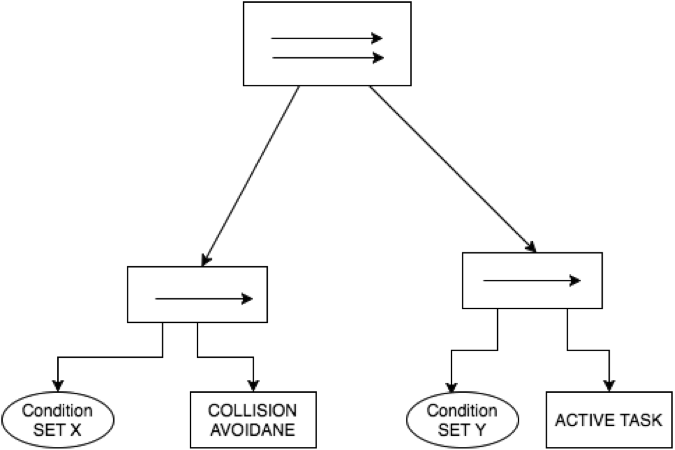
\includegraphics[width=3.25in]{Figures/BTAgent.png}
%\caption{Behaviour tree of an agent}
%\end{figure}

%Using the BT architecture, we define the behaviour of an agent as in Figure 7.
%We have two behaviours which are executed in parallel. One is the behaviour related to the mission execution and the other one is the behaviour related to safety.




IMPORTANT QUESTIONS to consider:
1. WHAT IS THE NOVELTY AND WHAT WE PROPOSE?
2. HOW TO VALIDATE?

Possible Answers:
\begin{itemize}


\item Being able to consider safety and mission in a single framework. being able to model both of those objectives in a separate way and being able to make analysis to satisfy both of the goals.
\item Two level of abstraction in our system:
\begin{itemize}
    \item Agent level
    \item Ensemble level
\end{itemize}
    and defining the MAPE-K loop FOR EACH OF THEM
    This way we can clear separation between responsibilities of an AGENT and responsibility of an ensemble as a group of AGENTs.

\end{itemize}

%QUESTIONS:
%1. HOW to perform the adaptation of two different behaviour: one related to safety(collision avoidance) and other one related to mission(tasks) (PLANNING COMPONENT)??? 

%Figure 1. Form of a Solver 
% SOLVERS ARE executable structures PROVIDED BY ENTITIES (Drones).
%SOLVER consists of three parts:
%-       DEMANDS: Boolean functions that check if a solver can be activated. It can be functions like checking if a particular component of a drone is working properly, it is feasible to perform some operation (the resources for performing the particular operation are available) etc…
%-      OPERATIONS: 
%		Actions (taking picture, measuring CO2); 
%		Movements (changing location (move forward 5 meters); rotate 90 degrees)
%Solver Invocation (call for another SOLVER)
%-      GUARANTEES: QUALITY score that gives information how well an AGENT can perform a TASK/SAFETY ACTION.



% needed in second column of first page if using \IEEEpubid
%\IEEEpubidadjcol

% An example of a floating figure using the graphicx package.
% Note that \label must occur AFTER (or within) \caption.
% For figures, \caption should occur after the \includegraphics.
% Note that IEEEtran v1.7 and later has special internal code that
% is designed to preserve the operation of \label within \caption
% even when the captionsoff option is in effect. However, because
% of issues like this, it may be the safest practice to put all your
% \label just after \caption rather than within \caption{}.
%
% Reminder: the "draftcls" or "draftclsnofoot", not "draft", class
% option should be used if it is desired that the figures are to be
% displayed while in draft mode.
%
%\begin{figure}[!t]
%\centering
%\includegraphics[width=2.5in]{myfigure}
% where an .eps filename suffix will be assumed under latex, 
% and a .pdf suffix will be assumed for pdflatex; or what has been declared
% via \DeclareGraphicsExtensions.
%\caption{Simulation Results}
%\label{fig_sim}
%\end{figure}

% Note that IEEE typically puts floats only at the top, even when this
% results in a large percentage of a column being occupied by floats.


% An example of a double column floating figure using two subfigures.
% (The subfig.sty package must be loaded for this to work.)
% The subfigure \label commands are set within each subfloat command, the
% \label for the overall figure must come after \caption.
% \hfil must be used as a separator to get equal spacing.
% The subfigure.sty package works much the same way, except \subfigure is
% used instead of \subfloat.
%
%\begin{figure*}[!t]
%\centerline{\subfloat[Case I]\includegraphics[width=2.5in]{subfigcase1}%
%\label{fig_first_case}}
%\hfil
%\subfloat[Case II]{\includegraphics[width=2.5in]{subfigcase2}%
%\label{fig_second_case}}}
%\caption{Simulation results}
%\label{fig_sim}
%\end{figure*}
%
% Note that often IEEE papers with subfigures do not employ subfigure
% captions (using the optional argument to \subfloat), but instead will
% reference/describe all of them (a), (b), etc., within the main caption.


% An example of a floating table. Note that, for IEEE style tables, the 
% \caption command should come BEFORE the table. Table text will default to
% \footnotesize as IEEE normally uses this smaller font for tables.
% The \label must come after \caption as always.
%
%\begin{table}[!t]
%% increase table row spacing, adjust to taste
%\renewcommand{\arraystretch}{1.3}
% if using array.sty, it might be a good idea to tweak the value of
% \extrarowheight as needed to properly center the text within the cells
%\caption{An Example of a Table}
%\label{table_example}
%\centering
%% Some packages, such as MDW tools, offer better commands for making tables
%% than the plain LaTeX2e tabular which is used here.
%\begin{tabular}{|c||c|}
%\hline
%One & Two\\
%\hline
%Three & Four\\
%\hline
%\end{tabular}
%\end{table}


% Note that IEEE does not put floats in the very first column - or typically
% anywhere on the first page for that matter. Also, in-text middle ("here")
% positioning is not used. Most IEEE journals use top floats exclusively.
% Note that, LaTeX2e, unlike IEEE journals, places footnotes above bottom
% floats. This can be corrected via the \fnbelowfloat command of the
% stfloats package.










% if have a single appendix:
%\appendix[Proof of the Zonklar Equations]
% or
%\appendix  % for no appendix heading
% do not use \section anymore after \appendix, only \section*
% is possibly needed

% use appendices with more than one appendix
% then use \section to start each appendix
% you must declare a \section before using any
% \subsection or using \label (\appendices by itself
% starts a section numbered zero.)
%





% Can use something like this to put references on a page
% by themselves when using endfloat and the captionsoff option.
\ifCLASSOPTIONcaptionsoff
  \newpage
\fi



% trigger a \newpage just before the given reference
% number - used to balance the columns on the last page
% adjust value as needed - may need to be readjusted if
% the document is modified later
%\IEEEtriggeratref{8}
% The "triggered" command can be changed if desired:
%\IEEEtriggercmd{\enlargethispage{-5in}}

% references section

% can use a bibliography generated by BibTeX as a .bbl file
% BibTeX documentation can be easily obtained at:
% http://www.ctan.org/tex-archive/biblio/bibtex/contrib/doc/
% The IEEEtran BibTeX style support page is at:
% http://www.michaelshell.org/tex/ieeetran/bibtex/
%\bibliographystyle{IEEEtran}
% argument is your BibTeX string definitions and bibliography database(s)
%\bibliography{IEEEabrv,../bib/paper}
%
% <OR> manually copy in the resultant .bbl file
% set second argument of \begin to the number of references
% (used to reserve space for the reference number labels box)
%\begin{thebibliography}{1}




 % Change the page header to say "Bibliography"

 % Use the "unsrtnat" BibTeX style for formatting the Bibliography
\bibliographystyle{IEEEtran}
\bibliography{IEEEabrv,Bibliography} 


%\bibitem{IEEEhowto:kopka}
%H.~Kopka and P.~W. Daly, \emph{A Guide to \LaTeX}, 3rd~ed.\hskip 1em plus
%  0.5em minus 0.4em\relax Harlow, England: Addison-Wesley, 1999.

%\end{thebibliography}

% biography section
% 
% If you have an EPS/PDF photo (graphicx package needed) extra braces are
% needed around the contents of the optional argument to biography to prevent
% the LaTeX parser from getting confused when it sees the complicated
% \includegraphics command within an optional argument. (You could create
% your own custom macro containing the \includegraphics command to make things
% simpler here.)
%\begin{biography}[{\includegraphics[width=1in,height=1.25in,clip,keepaspectratio]{mshell}}]{Michael Shell}
% or if you just want to reserve a space for a photo:

\begin{IEEEbiography}[{
\includegraphics[width=1in,height=1.25in,clip,keepaspectratio]{picture}}]{John Doe}
\blindtext
\end{IEEEbiography}








% You can push biographies down or up by placing
% a \vfill before or after them. The appropriate
% use of \vfill depends on what kind of text is
% on the last page and whether or not the columns
% are being equalized.

%\vfill

% Can be used to pull up biographies so that the bottom of the last one
% is flush with the other column.
%\enlargethispage{-5in}



% that's all folks
\end{document}


